\documentclass[11pt]{article}

\usepackage[]{authblk}
\usepackage{graphicx}
\usepackage{color}
\usepackage{longtable}
\usepackage{hanging}
\usepackage{indentfirst}
\usepackage{setspace}
\usepackage{enumitem}
\usepackage{verbatim}
\usepackage{upgreek}
\usepackage{framed}
\usepackage{ textcomp }
\usepackage{url}
\usepackage{soul}
\usepackage{amsmath, amsfonts,amssymb,mathrsfs}
\usepackage{fancyhdr}
\usepackage[compact]{titlesec}
\usepackage[T1]{fontenc}
\usepackage{lmodern}

\usepackage[backend=bibtex,hyperref=true,citestyle=authoryear,bibstyle=authortitle,firstinits=true,terseinits=true,doi=false,url=false,eprint=false,maxbibnames=10,maxcitenames=2]{biblatex}
\DeclareCiteCommand{\cite}
  {\usebibmacro{prenote}}
  {\usebibmacro{citeindex}%
   \printtext[bibhyperref]{\usebibmacro{cite}}}
  {\multicitedelim}
  {\usebibmacro{postnote}}

\DeclareCiteCommand*{\cite}
  {\usebibmacro{prenote}}
  {\usebibmacro{citeindex}%
   \printtext[bibhyperref]{\usebibmacro{citeyear}}}
  {\multicitedelim}
  {\usebibmacro{postnote}}

\DeclareCiteCommand{\parencite}[\mkbibparens]
  {\usebibmacro{prenote}}
  {\usebibmacro{citeindex}%
    \printtext[bibhyperref]{\usebibmacro{cite}}}
  {\multicitedelim}
  {\usebibmacro{postnote}}

\DeclareCiteCommand*{\parencite}[\mkbibparens]
  {\usebibmacro{prenote}}
  {\usebibmacro{citeindex}%
    \printtext[bibhyperref]{\usebibmacro{citeyear}}}
  {\multicitedelim}
  {\usebibmacro{postnote}}

\DeclareCiteCommand{\footcite}[\mkbibfootnote]
  {\usebibmacro{prenote}}
  {\usebibmacro{citeindex}%
  \printtext[bibhyperref]{ \usebibmacro{cite}}}
  {\multicitedelim}
  {\usebibmacro{postnote}}

\DeclareCiteCommand{\footcitetext}[\mkbibfootnotetext]
  {\usebibmacro{prenote}}
  {\usebibmacro{citeindex}%
   \printtext[bibhyperref]{\usebibmacro{cite}}}
  {\multicitedelim}
  {\usebibmacro{postnote}}

\DeclareCiteCommand{\textcite}
  {\boolfalse{cbx:parens}}
  {\usebibmacro{citeindex}%
   \printtext[bibhyperref]{\usebibmacro{textcite}}}
  {\ifbool{cbx:parens}
     {\bibcloseparen\global\boolfalse{cbx:parens}}
     {}%
   \multicitedelim}
  {\usebibmacro{textcite:postnote}}

\newcommand{\citep}{\parencite}
\newcommand{\citet}{\textcite}
\defbibheading{relevref}[\refname]{\section*{Relevant References}}

\renewcommand{\postnotedelim}{\iffieldpages{postnote}{\addcolon}{\addcomma\space}} 
\DeclareFieldFormat{postnote}{#1} 

\DeclareFieldFormat[article, inbook, incollection, inproceedings, patent, thesis, unpublished]{title}{#1}
\DeclareFieldFormat[article, inbook, incollection, inproceedings, patent, thesis, unpublished]{journaltitle}{\mkbibemph{#1}\nopunct}
\DeclareFieldFormat[article, inbook, incollection, inproceedings, patent, thesis, unpublished]{volume}{{#1}\addcolon} %puts volume number in parens
%\DeclareFieldFormat[article, inbook, incollection, inproceedings, patent, thesis, unpublished]{year}{\mkbibparens{#1}\nopunct} %puts year in parens

\DeclareFieldFormat[article, incollection, patent, thesis, unpublished]{pages}{{\nopp#1}}

\DeclareFieldFormat{sentencecase}{\MakeSentenceCase{#1}}

\renewbibmacro*{title}{%
  \ifthenelse{\iffieldundef{title}\AND\iffieldundef{subtitle}}
    {}
    {\ifthenelse{\ifentrytype{article}\OR\ifentrytype{inbook}%
      \OR\ifentrytype{incollection}\OR\ifentrytype{inproceedings}%
      \OR\ifentrytype{inreference}}
      {\printtext[title]{%
        \printfield[sentencecase]{title}%
        \setunit{\subtitlepunct}%
        \printfield[sentencecase]{subtitle}}}%
      {\printtext[title]{%
        \printfield[titlecase]{title}%
        \setunit{\subtitlepunct}%
        \printfield[titlecase]{subtitle}}}%
     \newunit}%
  \printfield{titleaddon}}

\DefineBibliographyStrings{english}{% various adjustments to common bib entry strings
urlseen = {Accessed:},% What goes in front of the date a URL was accessed/retrieved etc.
editor = {(Ed)},%Ed – no dot, in brackets
editors = {(Eds)},% Eds – no dot, in brackets
byeditor = {(Ed.)}}% ‘Edited by’ for edited works

\DeclareNameAlias{default}{last-first}

\renewbibmacro{in:}{}

\renewbibmacro{publisher+location+date}{
  \iflistundef{publisher}
    {}
    {\printlist{publisher}%
       {\addcomma\space}%
      \iflistundef{location}
        {}
        {\printlist{location}}%
    }
}

\DeclareBibliographyDriver{article}{%
\usebibmacro{bibindex}%
\usebibmacro{begentry}%
\usebibmacro{author/translator+others}%
\newunit\newblock
\printfield{year}%
\setunit{\labelnamepunct}\newblock
\usebibmacro{title}%
\newunit
\printlist{language}%
\newunit\newblock
\usebibmacro{byauthor}%
\newunit\newblock
\usebibmacro{bytranslator+others}%
\newunit\newblock
\printfield{version}%
\newunit\newblock
%\usebibmacro{in:}% %mit in:
\usebibmacro{journal}%
\newunit\newblock
\printfield{volume}%
\newunit\newblock
\usebibmacro{byeditor+others}%
\newunit\newblock
\usebibmacro{note+pages}%
\newunit\newblock
\iftoggle{bbx:isbn}
{}%
\newunit\newblock
\usebibmacro{doi+eprint+url}%
\newunit\newblock
\usebibmacro{addendum+pubstate}%
\newunit\newblock
\usebibmacro{pageref}%
\usebibmacro{finentry}}

\DeclareBibliographyDriver{inproceedings}{%
\usebibmacro{bibindex}%
\usebibmacro{begentry}%
\usebibmacro{author/translator+others}%
\newunit\newblock
\printfield{year}%
\setunit{\labelnamepunct}\newblock
\usebibmacro{title}%
\newunit
\printlist{language}%
\newunit\newblock
\usebibmacro{byauthor}%
\newunit\newblock
\usebibmacro{bytranslator+others}%
\newunit\newblock
\printfield{version}%
\newunit\newblock
%\usebibmacro{in:}% %mit in:
\usebibmacro{booktitle}%
\newunit\newblock
\printfield{volume}%
\newunit\newblock
\usebibmacro{byeditor+others}%
\newunit\newblock
\usebibmacro{publisher+location+date}%
\newunit\newblock
\usebibmacro{note+pages}%
\newunit\newblock
\usebibmacro{pageref}%
\usebibmacro{finentry}}

\DeclareBibliographyDriver{book}{%
\usebibmacro{bibindex}%
\usebibmacro{begentry}%
\usebibmacro{author/translator+others}%
\newunit\newblock
\printfield{year}%
\setunit{\labelnamepunct}\newblock
\usebibmacro{title}%
\newunit
\printlist{language}%
\newunit\newblock
\usebibmacro{byauthor}%
\newunit\newblock
\usebibmacro{bytranslator+others}%
\newunit\newblock
%\usebibmacro{in:}% %mit in:
\usebibmacro{booktitle}%
\newunit\newblock
\printfield{volume}%
\newunit\newblock
\usebibmacro{publisher+location+date}%
\newunit\newblock
\usebibmacro{note+pages}%
\newunit\newblock
\usebibmacro{pageref}%
\usebibmacro{finentry}}





\setlength{\evensidemargin}{0in}
\setlength{\headheight}{0in}
\setlength{\headsep}{0in}
\setlength{\oddsidemargin}{-0.25in}
\setlength{\paperheight}{11in}
\setlength{\paperwidth}{8.5in}
\setlength{\tabcolsep}{0in}
\setlength{\textheight}{9in}
\setlength{\textwidth}{7in}
\setlength{\topmargin}{0in}
\setlength{\topskip}{0in}
\setlength{\voffset}{0in}
\parskip = 0.15in
\pagestyle{plain}
\setlength{\parindent}{0cm}

\definecolor{citescol}{RGB}{194,101,1}
\definecolor{urlscol}{RGB}{0,150,206}
\definecolor{linkscol}{RGB}{149,0,207}
\definecolor{mycol}{RGB}{25,23,191}
\definecolor{outputcol}{RGB}{34,139,34}
\definecolor{tcol}{RGB}{165,0,14}


\DeclareMathAlphabet{\msfsl}{T1}{cmr}{m}{it}
\DeclareMathAlphabet{\msyf}{OMX}{pcr}{m}{it}
\newcommand{\alf}{\upalpha}
\newcommand{\hilight}[1]{\colorbox{yellow}{#1}}

\newcommand{\levelone}[1]{
\bigskip
\noindent{\LARGE{\textsc{#1}}}
\vspace {0.05in}
}

\newcommand{\leveltwo}[1]{
\bigskip
\noindent{\Large{\textit{#1}}}
\vspace {-1mm}
}

\newcommand{\descriptionhead}[1]{
\noindent{\textcolor{mycol}{\textbf{\textit{#1}}}}\\ \vspace{-7mm}
}

\newcommand{\dhead}[1]{
\noindent{\textbf{\textit{#1 --}}}
}



\newcommand{\exs}[1]{
\vspace{-4mm}
\begin{itemize}
\item #1 \\ \vspace{-8mm}
\end{itemize}
}

\newcommand{\nbo}[1]{{\color{red}{#1}}}


\newcommand{\stepbullet}{\noindent \textbullet \ }
\newcommand{\mi}[1]{\textbf{\textit{#1}}}


\newcommand{\levelthree}[1]{\textit{#1 --}}


%\bibliographystyle{apalike}
%\bibpunct[; ]{(}{)}{;}{a}{,}{;}


\usepackage[breaklinks]{hyperref}
\usepackage[all]{hypcap}
\hypersetup{colorlinks=true,linkcolor=linkscol,citecolor=citescol,urlcolor=urlscol}


\newcommand{\R}{\texttt{R} }
\newcommand{\TESS}{\texttt{TESS}}
\newcommand{\PBD}{\texttt{PBD}}
\newcommand{\DDD}{\texttt{DDD}}
\newcommand{\Laser}{\texttt{laser}}
\newcommand{\TreePar}{\texttt{TreePar}}
\newcommand{\diversitree}{\texttt{diversitree}}
\newcommand{\RevBayes}{\texttt{RevBayes}}
\newcommand{\Rev}{\texttt{Rev}}
\newcommand{\MrBayes}{\texttt{MrBayes}}
\newcommand{\BEAST}{\texttt{BEAST}}
\newcommand{\PhyloBayes}{\texttt{PhyloBayes}}
\newcommand{\PAML}{\texttt{PAML}}

\let\otheriint\iint
\let\iint\relax
\usepackage{ wasysym }

\usepackage{framed}
\usepackage[]{listings}
%\usepackage{fontspec}
\usepackage{placeins}
\usepackage{epstopdf}

\lstset{breaklines=true}

\definecolor{shadecolor}{RGB}{194,225,255}

\setlength{\tabcolsep}{5pt}
\setlength{\topmargin}{-0.4in}
\setlength{\headheight}{14.5pt}
\pagestyle{fancy}

\newcommand{\taha}[1]{{\textcolor{red}{[TAH comment: #1]}}} % TAH comment

\titlespacing{\section}{0pt}{*0}{*0}
\titlespacing{\subsection}{0pt}{*0}{*0}
\titlespacing{\subsubsection}{0pt}{*0}{*0}

\titleformat{\section}
  {\normalfont\Large\bfseries\color{mycol}}
  {\thesection}{1em}{}

\titleformat{\subsection}
  {\normalfont\large\bfseries\color{mycol}}
  {\thesubsection}{1em}{}

\titleformat{\subsubsection}
  {\normalfont\bfseries\color{mycol}}
  {\thesubsubsection}{1em}{}

% command for MrBayes command-line step
\newcommand{\cl}[1]{{\texttt{\textbf{#1}}}}

\newcommand{\colx}[1]{{\textcolor{tcol}{#1}}}

\newcommand{\mbcl}[1]{\exs{\cl{MrBayes > {#1}}}}

\newcommand{\rbprmt}{RevBayes > } 
\newcommand{\rbcl}[1]{\exs{\cl{\rbprmt{#1}}}}
\newcommand{\rbout}[1]{\exs{\cl{\textcolor{outputcol}{#1}}}}
\newcommand{\rbdn}{{\Large \symbol{126}}} % This makes a copy/pasteable tilde
\newcommand{\rbclml}[1]{\exs{\cl{\ \ \ \ \ \ \ \ \ \ \ {#1}}}}

% text box settings
% requires compiling w/ XeLaTeX
%\newfontfamily\listingsfont[Scale=1.0]{Courier New}
%\lstset{basicstyle=\listingsfont, columns=texcl}
%\defaultfontfeatures{Mapping=tex-text}


\makeatletter
\lst@CCPutMacro\lst@ProcessOther {"2D}{\lst@ttfamily{-{}}{-{}}}
\@empty\z@\@empty
\makeatother


\addbibresource{master-refs.bib}


\usepackage{tikz}

\setlength{\topmargin}{-0.4in}
\setlength{\headheight}{14.5pt}
\pagestyle{fancy}

\usepackage[breaklinks]{hyperref}
\usepackage[all]{hypcap}
\hypersetup{colorlinks=true,linkcolor=linkscol,citecolor=citescol,urlcolor=urlscol}

\definecolor{lg}{gray}{0.75}
\def\gcirc{{%
    \setbox0\hbox{$\fullmoon$}%
    \rlap{\hbox to \wd0{\hss{$\textcolor{lg}{\newmoon}$}\hss}}\box0
}}


\begin{document}
\renewcommand{\headrulewidth}{0.5pt}
\headsep = 20pt
\lhead{ }
\rhead{\textsc {BEAST v2 Tutorial}}

\thispagestyle{plain}

\begin{center}
\textbf{\LARGE Tutorial using BEAST v2.$*$}\\\vspace{2mm}
\textbf{\textcolor{mycol}{\Large Prior selection and clock calibration using Influenza A data}}\\
\vspace{4mm}
{\Large {\em Veronika Bo\v{s}kov\'a and Venelin Mitov}}
\end{center}

\bigskip
\section{Background}
In the Bayesian analysis of sequence data, priors play an important role. When wrongly selected, the runs may take very long to converge, not converge at all or cause a bias in the inferred trees and model parameters. Selection of proper priors and starting values is crucial and can be a difficult exercise at the start. It is not always easy to pick a proper model of tree generation (tree prior), substitution model, molecular clock model or the prior distribution for an unknown parameter. 

The molecular clock model aims to estimate the substitution rate of the data. It is important to understand under which circumstances to use which model and when molecular calibration works. This will help the investigator determine which estimates of parameters can be trusted and which can not.

In this tutorial, we will explore how priors are selected and how molecular clock calibration works using the H3N2 influenza A data from the flu virus spreading in the USA in 2009. 

%\clearpage
%\newpage
\bigskip
\section{Programs used in this Exercise}\label{programsSec}

\descriptionhead{BEAST -- Bayesian Evolutionary Analysis Sampling Trees}

BEAST version 2.4.2 \citep{drummond06,drummond07,Bouckaert2014}. 

\descriptionhead{BEAUti -- Bayesian Evolutionary Analysis Utility}

To help us to specify the XML file for BEAST.

\descriptionhead{Tracer} 

Tracer (\url{http://tree.bio.ed.ac.uk/software/tracer}) is used to summarize the posterior estimates of the various parameters sampled by the Markov Chain. This program can be used for visual inspection and assessment of convergence. It helps to quickly view median estimate and 95\% credible intervals (which approximate the 95\% highest posterior density intervals) of the parameters, and calculates the effective sample sizes (ESS) of parameters. It also helps to visualise potential parameter correlations.

\descriptionhead{TreeAnnotator}

TreeAnnotator is used to summarize the posterior sample of trees to produce a maximum clade credibility tree. It is also useful to summarize and visualise the posterior estimates of other tree parameters (e.g. node height). 

\descriptionhead{FigTree}

FigTree is a program for viewing trees and producing publication-quality figures. It can interpret the node-annotations created on the summary trees by TreeAnnotator, allowing the user to display node-based statistics (e.g. posterior probabilities) (\url{http://tree.bio.ed.ac.uk/software/figtree}).



\newpage
\section{Practical: H3N2 flu dynamics - heterochronous data}\label{heterochronous}
In this tutorial, we will estimate the rate of evolution from a set of virus sequences which have been isolated either at one point in time (homochronous) or at different points in time (heterochronous or time-stamped data). We use the hemagglutinin (HA) gene of the H3N2 strain spreading across America along the pandemic H1N1 virus in 2009 \citep{cdc2009}. 

The aim of this tutorial is to obtain estimates for : 
\begin{itemize}
 	\item the rate of molecular evolution
	\item the phylogenetic relationships with measures of internal node heights
	\item the date of the most recent common ancestor of the sampled virus sequences.
\end{itemize}

More general aim of this tutorial is:
\begin{itemize}
	\item to understand how to set the priors and why this is important
	\item to understand why and when the rate of evolution can be estimated from the data.
\end{itemize}



\bigskip
\subsection{The Data}

The full heterochronous dataset contains an alignment of 139 HA sequences 1738 nucleotides long. The samples were obtained from California between April and June 2009 (file named \\
\texttt{InfluenzaAH3N2\_HAgene\_2009\_California\_heterochronous.nexus}). The homochronous data is a subset of the heterochronous data, consisting of an alignment of 29 sequences of 1735 nucleotides all sampled on April 28, 2009 (file named \texttt{InfluenzaAH3N2\_HAgene\_2009\_California\_homochronous.nexus}). 

%\begin{framed}
%Download data files from:
%\begin{center}
%{\textcolor{red}{\underline{\bf 
%%\url{
%the link to data should come here
%%} 
%}}}
%\end{center}
%\end{framed}



\bigskip
\subsection{Creating the Analysis File with BEAUti}

We will use BEAUti program to select the priors and starting values for our analysis, and save these settings into a BEAST-readable XML format file. 

\begin{framed}
Begin by starting up the BEAUti program.
\end{framed}



\bigskip
\subsubsection{Installing BEAST 2 Plug-Ins}

Since we will be using the birth-death skyline model \citep{Stadler2013}, we need to make sure it is available in BEAUti. It is not one of the default models but rather an add-on (also called a plug-in or package). You only need to install a BEAST 2 package once. Thus, if you close BEAUti, you do not have to load \textbf{BDSKY} the next time you open the program. However, it is worth checking the package manager for updates to plug-ins, particularly if you update your version of BEAST 2.

\textbf{BDSKY} model was used in the previous tutorial, so you should already have it up and running in BEAUti. Also, we do not expect that there were any updates to the version you loaded just few hours ago, so you can skip the following few lines and go directly to section \ref{Importing alignment}. However, in case you have not managed to get it running yet, follow these instructions to install the \textbf{BDSKY} add-on. 

\begin{framed}
Open the \textbf{BEAST 2 Package Manager} by navigating to \textbf{File\textrightarrow Manage Packages}. [Figure \ref{packageManage1}]
\end{framed}

\begin{figure}[h!]
\centering
\fbox{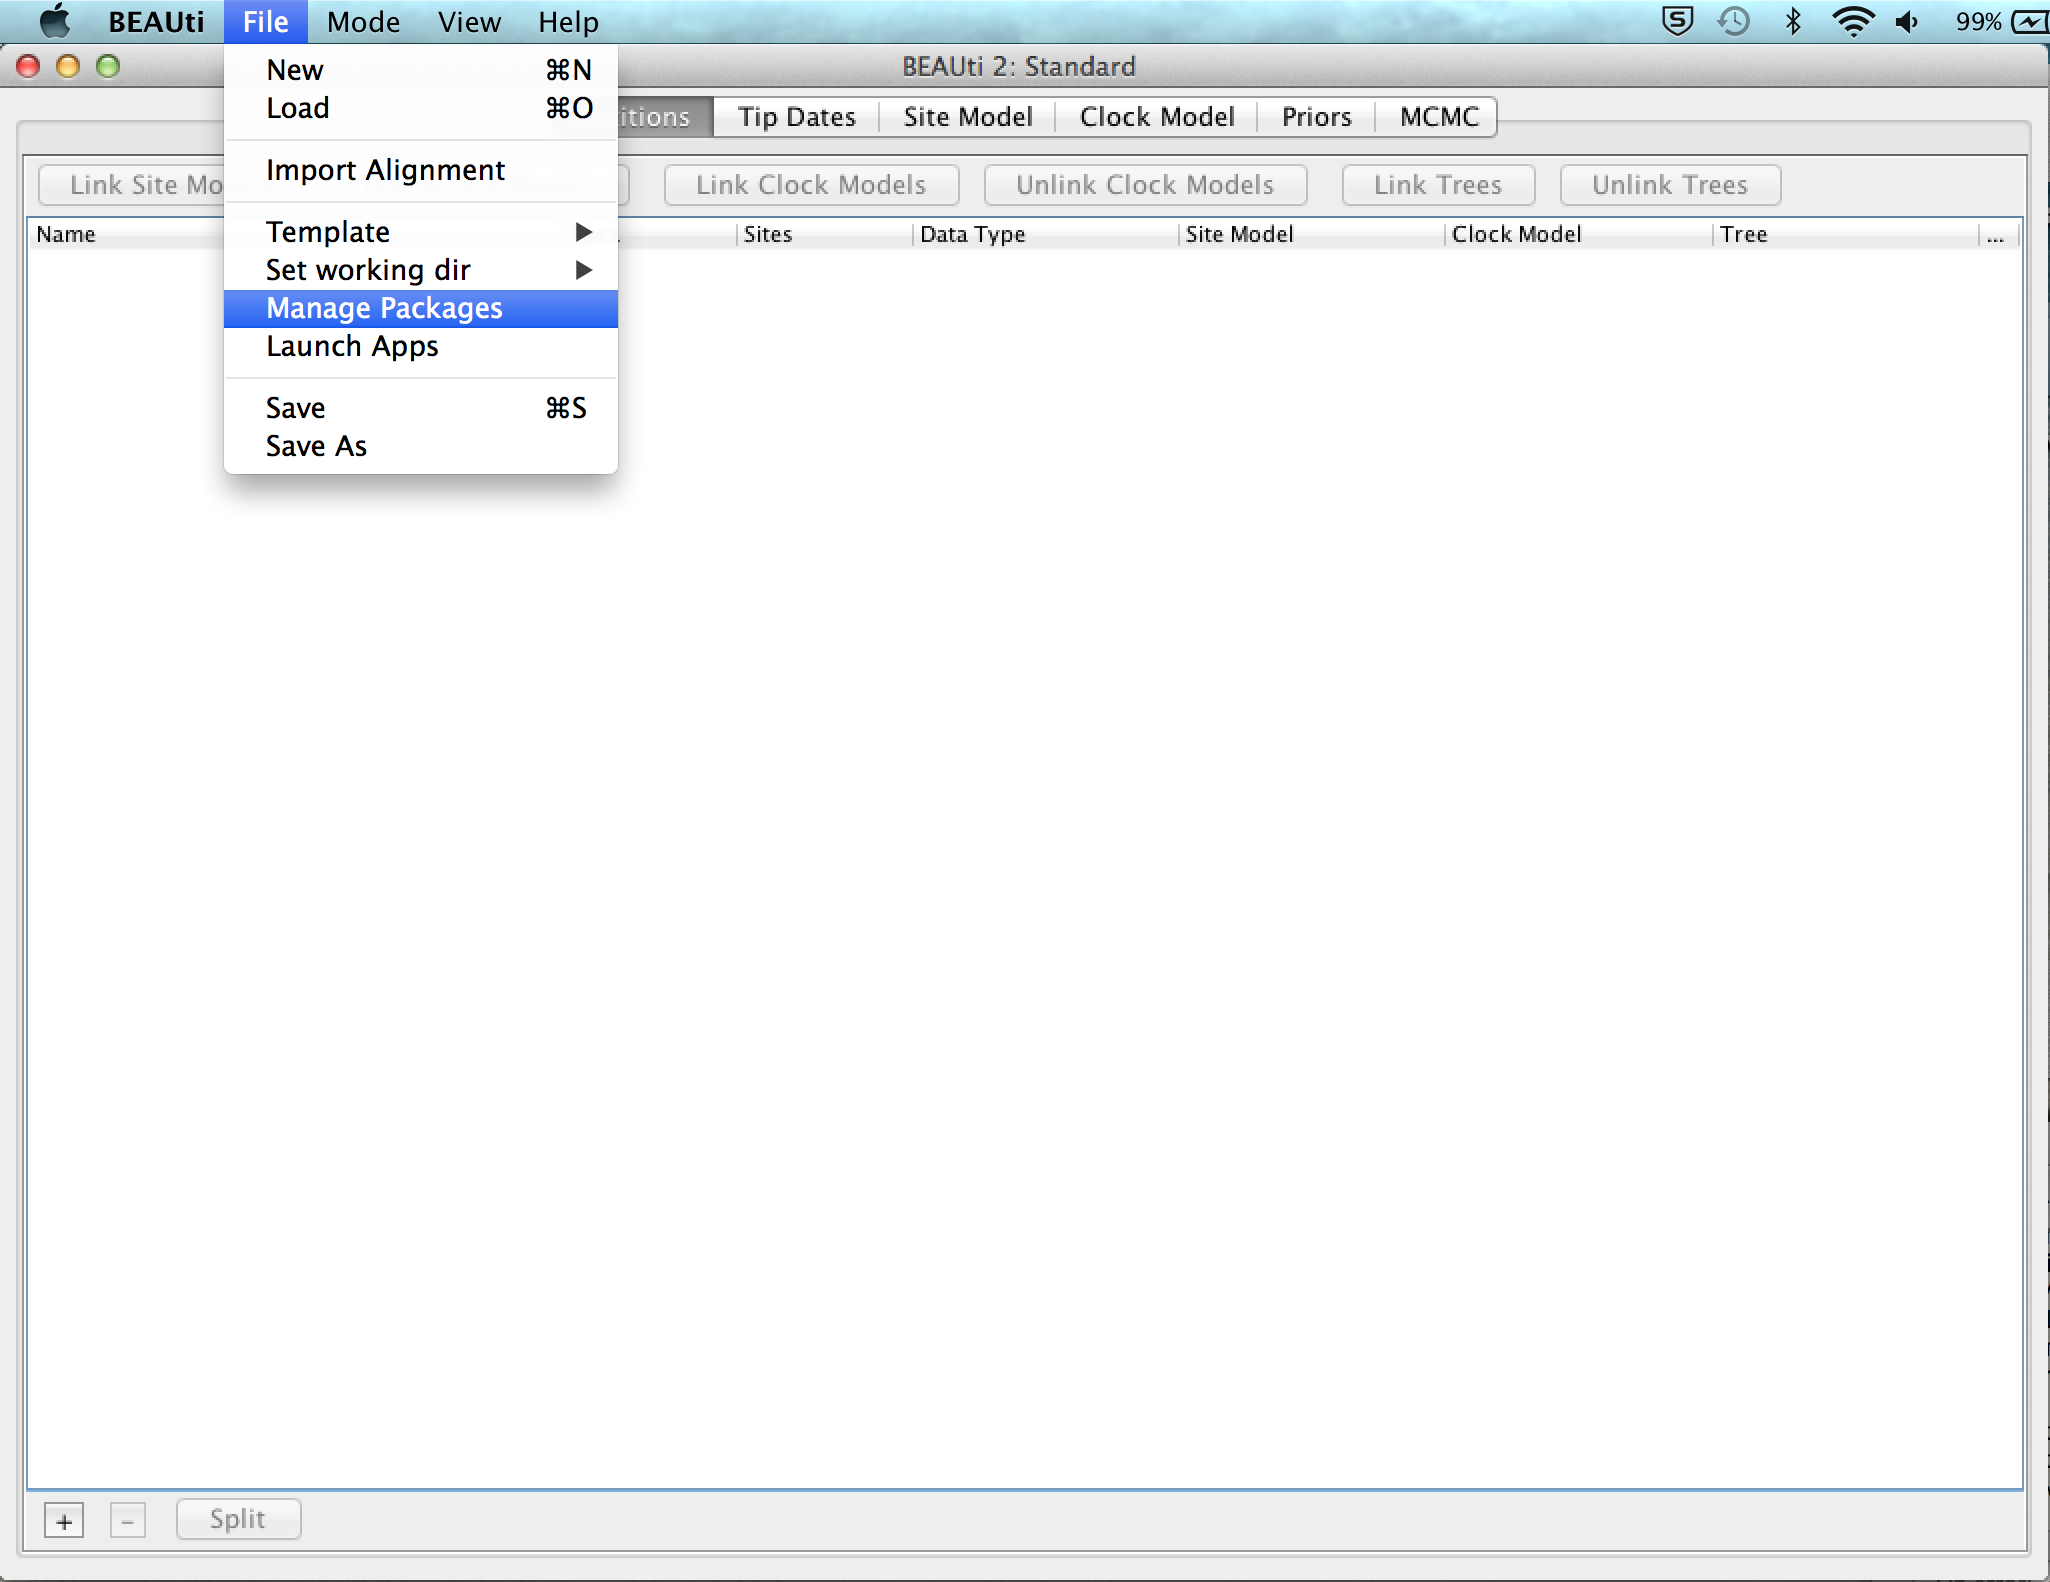
\includegraphics[width=0.75\textwidth]{figures/beast2_package_manager_opening.png}}
\caption{\small Finding the BEAST2 Package Manager.}
\label{packageManage1}
\end{figure}

\begin{framed}
Install the \textbf{BDSKY} package by selecting it and clicking the \textbf{Install/Upgrade} button. [Figure \ref{packageManage2}]
\end{framed}

\begin{figure}[h!]
\centering
\fbox{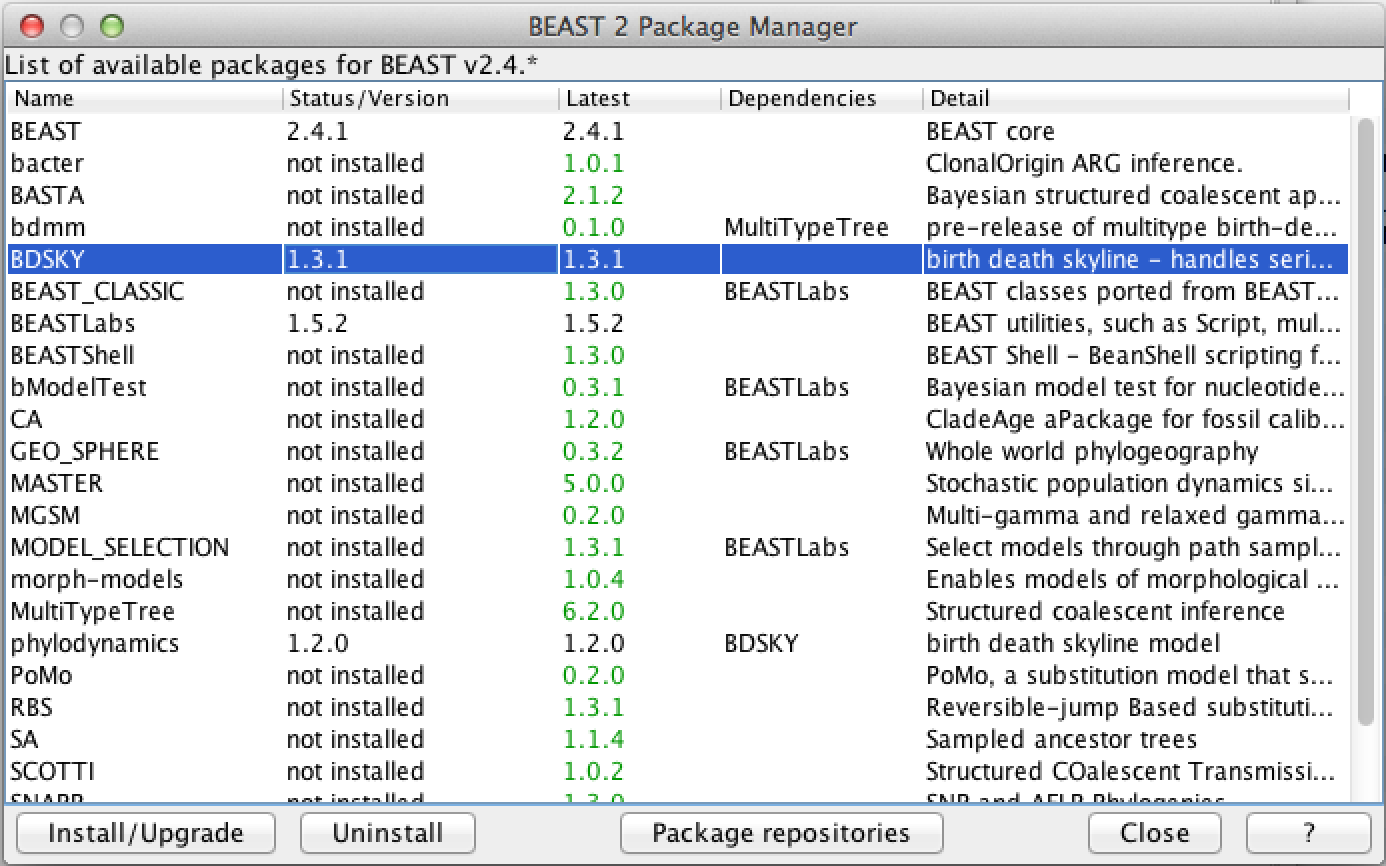
\includegraphics[width=0.75\textwidth]{figures/beast2_package_manager.png}}
\caption{\small The BEAST2 Package Manager.}
\label{packageManage2}
\end{figure}

After the installation of an add-on, the program is on your computer, but BEAUti is unable to load the template files for the newly installed model unless it is restarted. So, let's restart BEAUti to make sure we have \textbf{BDSKY} model at hand.

\begin{framed}
Close the \textbf{BEAST 2 Package Manager} and {\textcolor{red}{\underline{\bf restart BEAUti}}} to fully load the \textbf{BDSKY} package.
\end{framed}



\newpage
\bigskip
\subsubsection{Importing alignment}\label{Importing alignment}

We will first analyse the alignment of sequences sampled through time (heterochronous sequences). 
 
\begin{framed}
In the \textbf{Partitions} panel, import the nexus file with the alignment by navigating to \textbf{File\textrightarrow Import Alignment} in the menu [Figure \ref{importAlignment}] and then finding the file called \newline \texttt{InfluenzaAH3N2\_HAgene\_2009\_California\_heterochronous.nexus}  file on your computer.
\end{framed}

\begin{figure}[h!]
\centering
\fbox{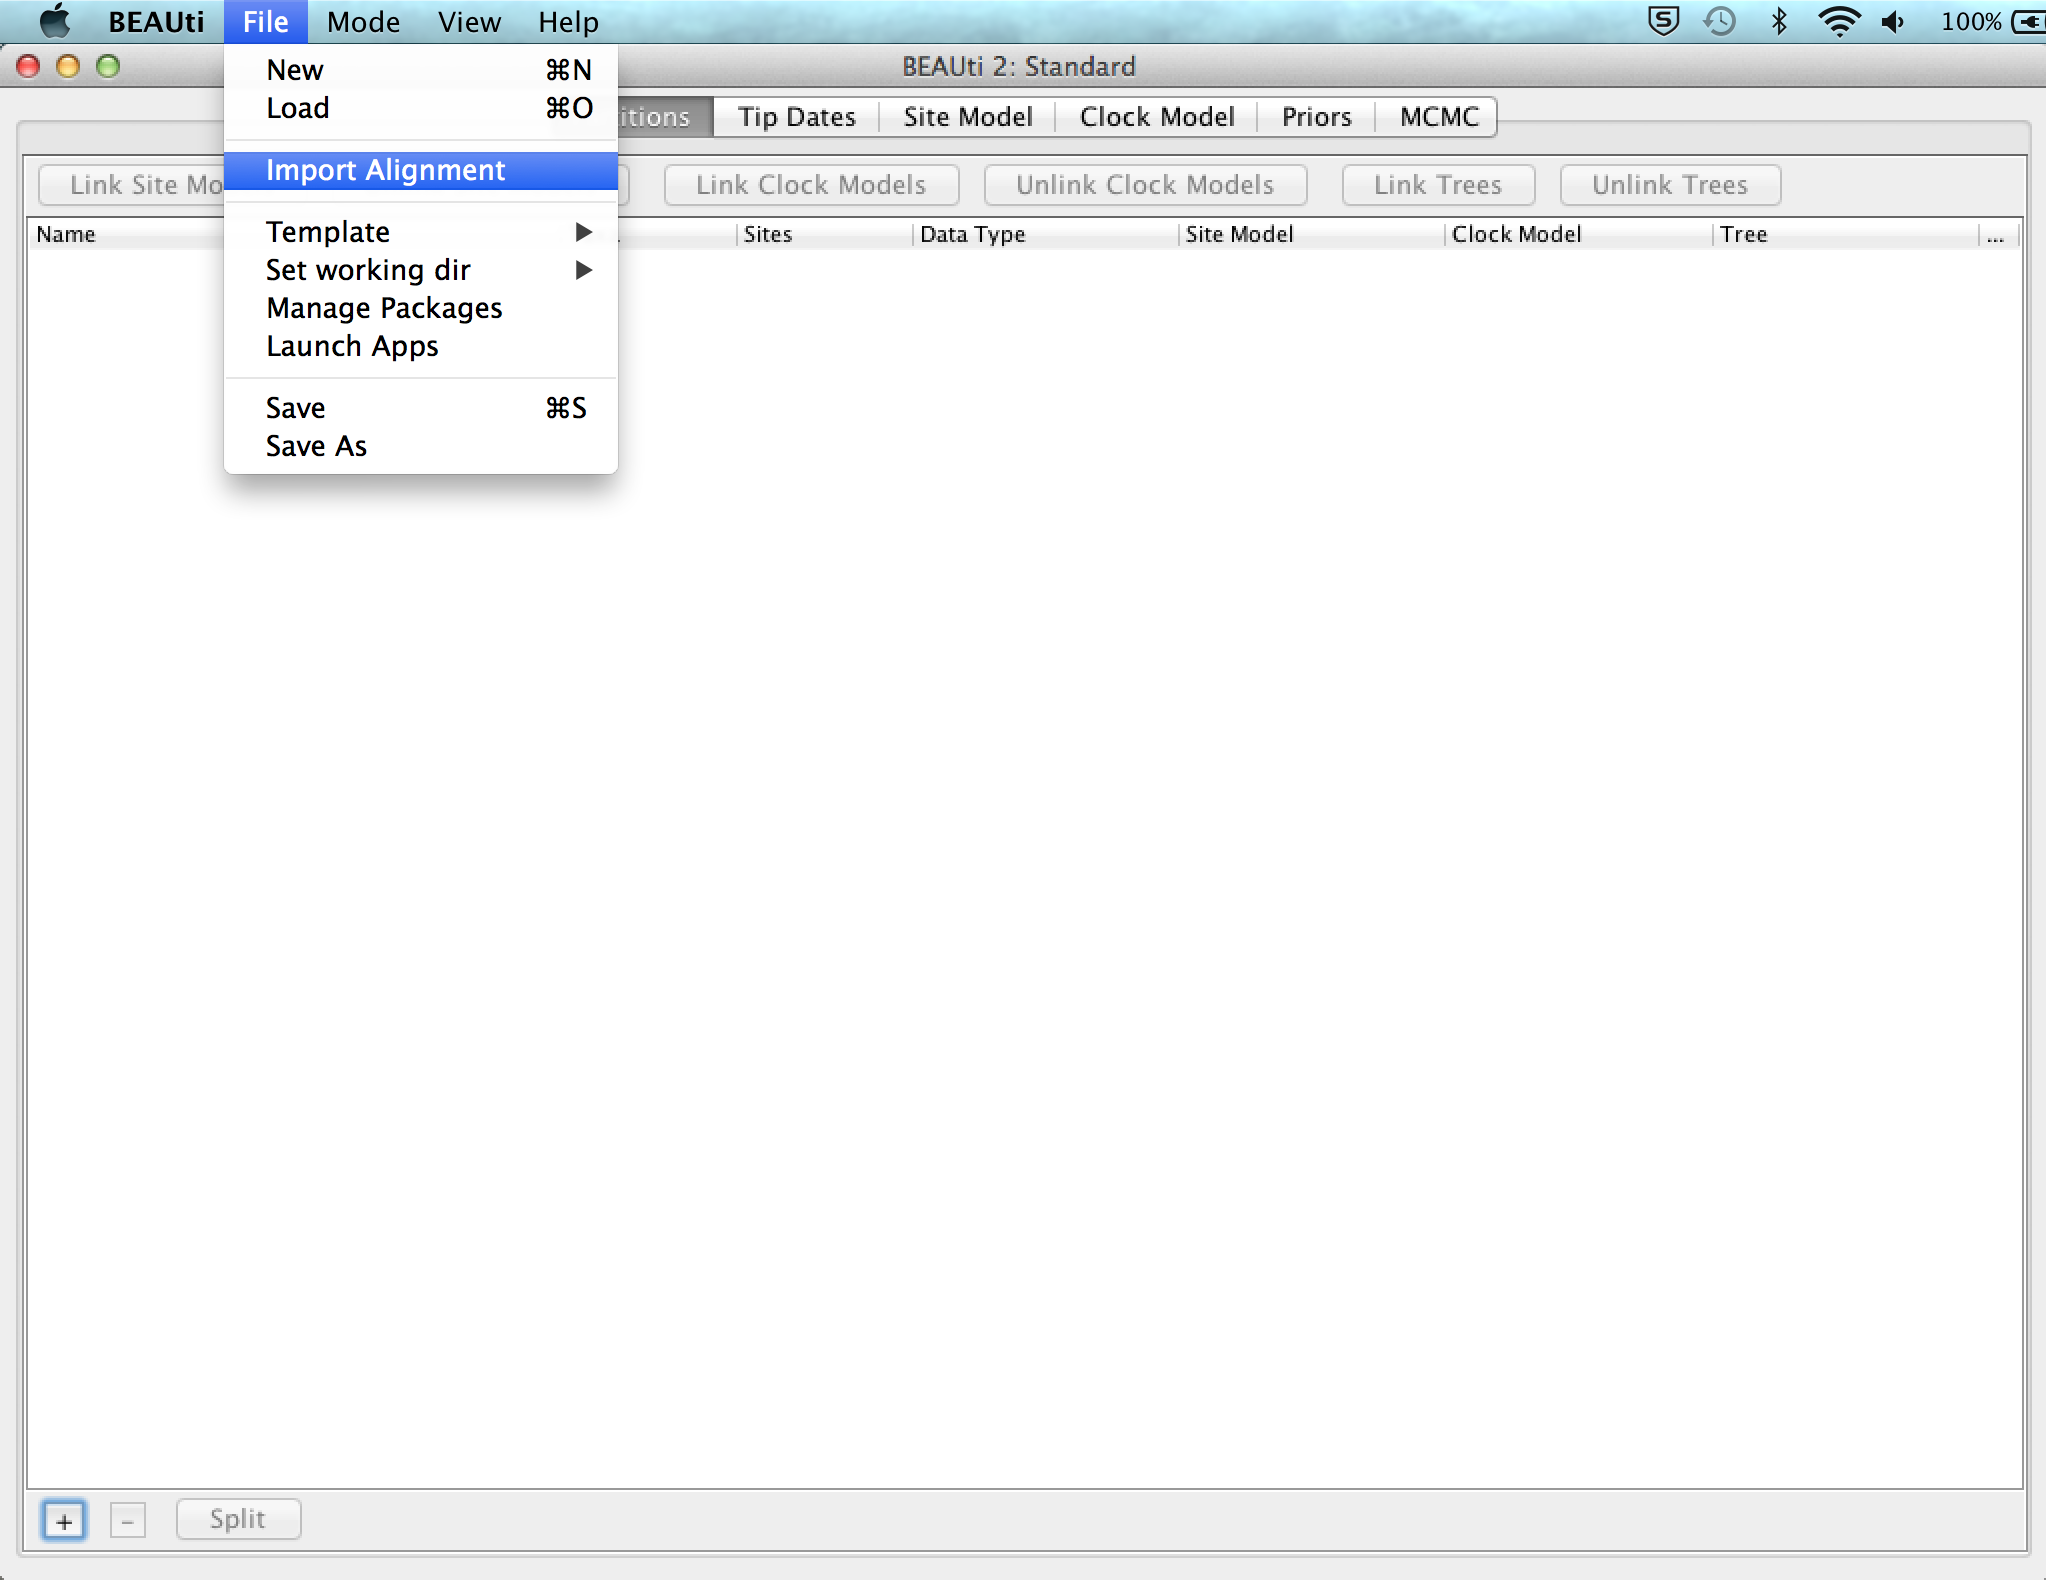
\includegraphics[width=0.75\textwidth]{figures/beast2_import_alignment.png}}
\caption{\small Importing alignment into BEAUti.}
\label{importAlignment}
\end{figure}

You can view the alignment by double-clicking on the name of the alignment in BEAUti. Since we only have one partition there is nothing more we can do in the \textbf{Partitions} panel and proceed to specifying the tip dates. 



\bigskip
\subsubsection{Setting up tip dates}

The heterochronous dataset contains the information on when the sequences were sampled. We want to use this information to specify the tip dates in BEAUti. 

\begin{framed}
In the \textbf{Tip Dates} panel, click the \textbf{Use tip dates} option. 
\end{framed}

We want all the tree information to be specified for units of time in ``years'', thus we leave the \textbf{Dates specified as} option set to default ``year''. Also we want the time to flow forward in time in the tree, therefore, we keep to default option of tip dates being specified as ``Since some time in the past'' [Figure \ref{timeUnitsAndFlow}].

\begin{figure}[h!]
\centering
\fbox{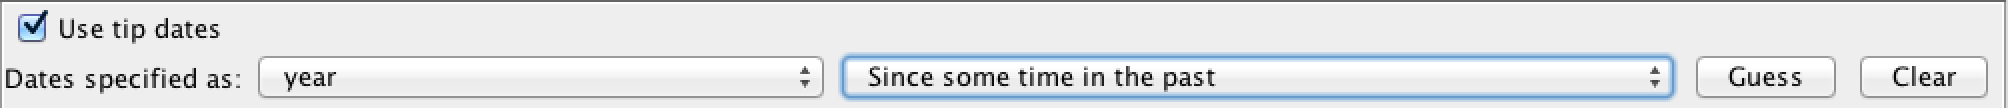
\includegraphics[width=0.75\textwidth]{figures/beast2_time_specification.png}}
\caption{\small Specifying time units and direction of time flow.}
\label{timeUnitsAndFlow}
\end{figure}

You could specify the tip dates by hand, by clicking for each row (i.e. for each sequence) into the \textbf{Date} column and typing the date information in for each sequence in turn. However, this is a laborious and error-prone procedure and can take a long time to finish. Fortunately, we can use BEAUti, to read off the dates from the sequence names for us. Each sequence is named such that the expression after the last underscore character (``\_'') contains the sampling date information. BEAUti can search for this expression to extract the sequence date.

\begin{framed}
Press the \textbf{Guess} button. A window will appear where you can specify how BEAUti can find the date of sampling of each sequence. [Figure \ref{guessDates}]

Select \textbf{use everything} and specify \textbf{after last} \_.
\end{framed}

\begin{figure}[h!]
\centering
\fbox{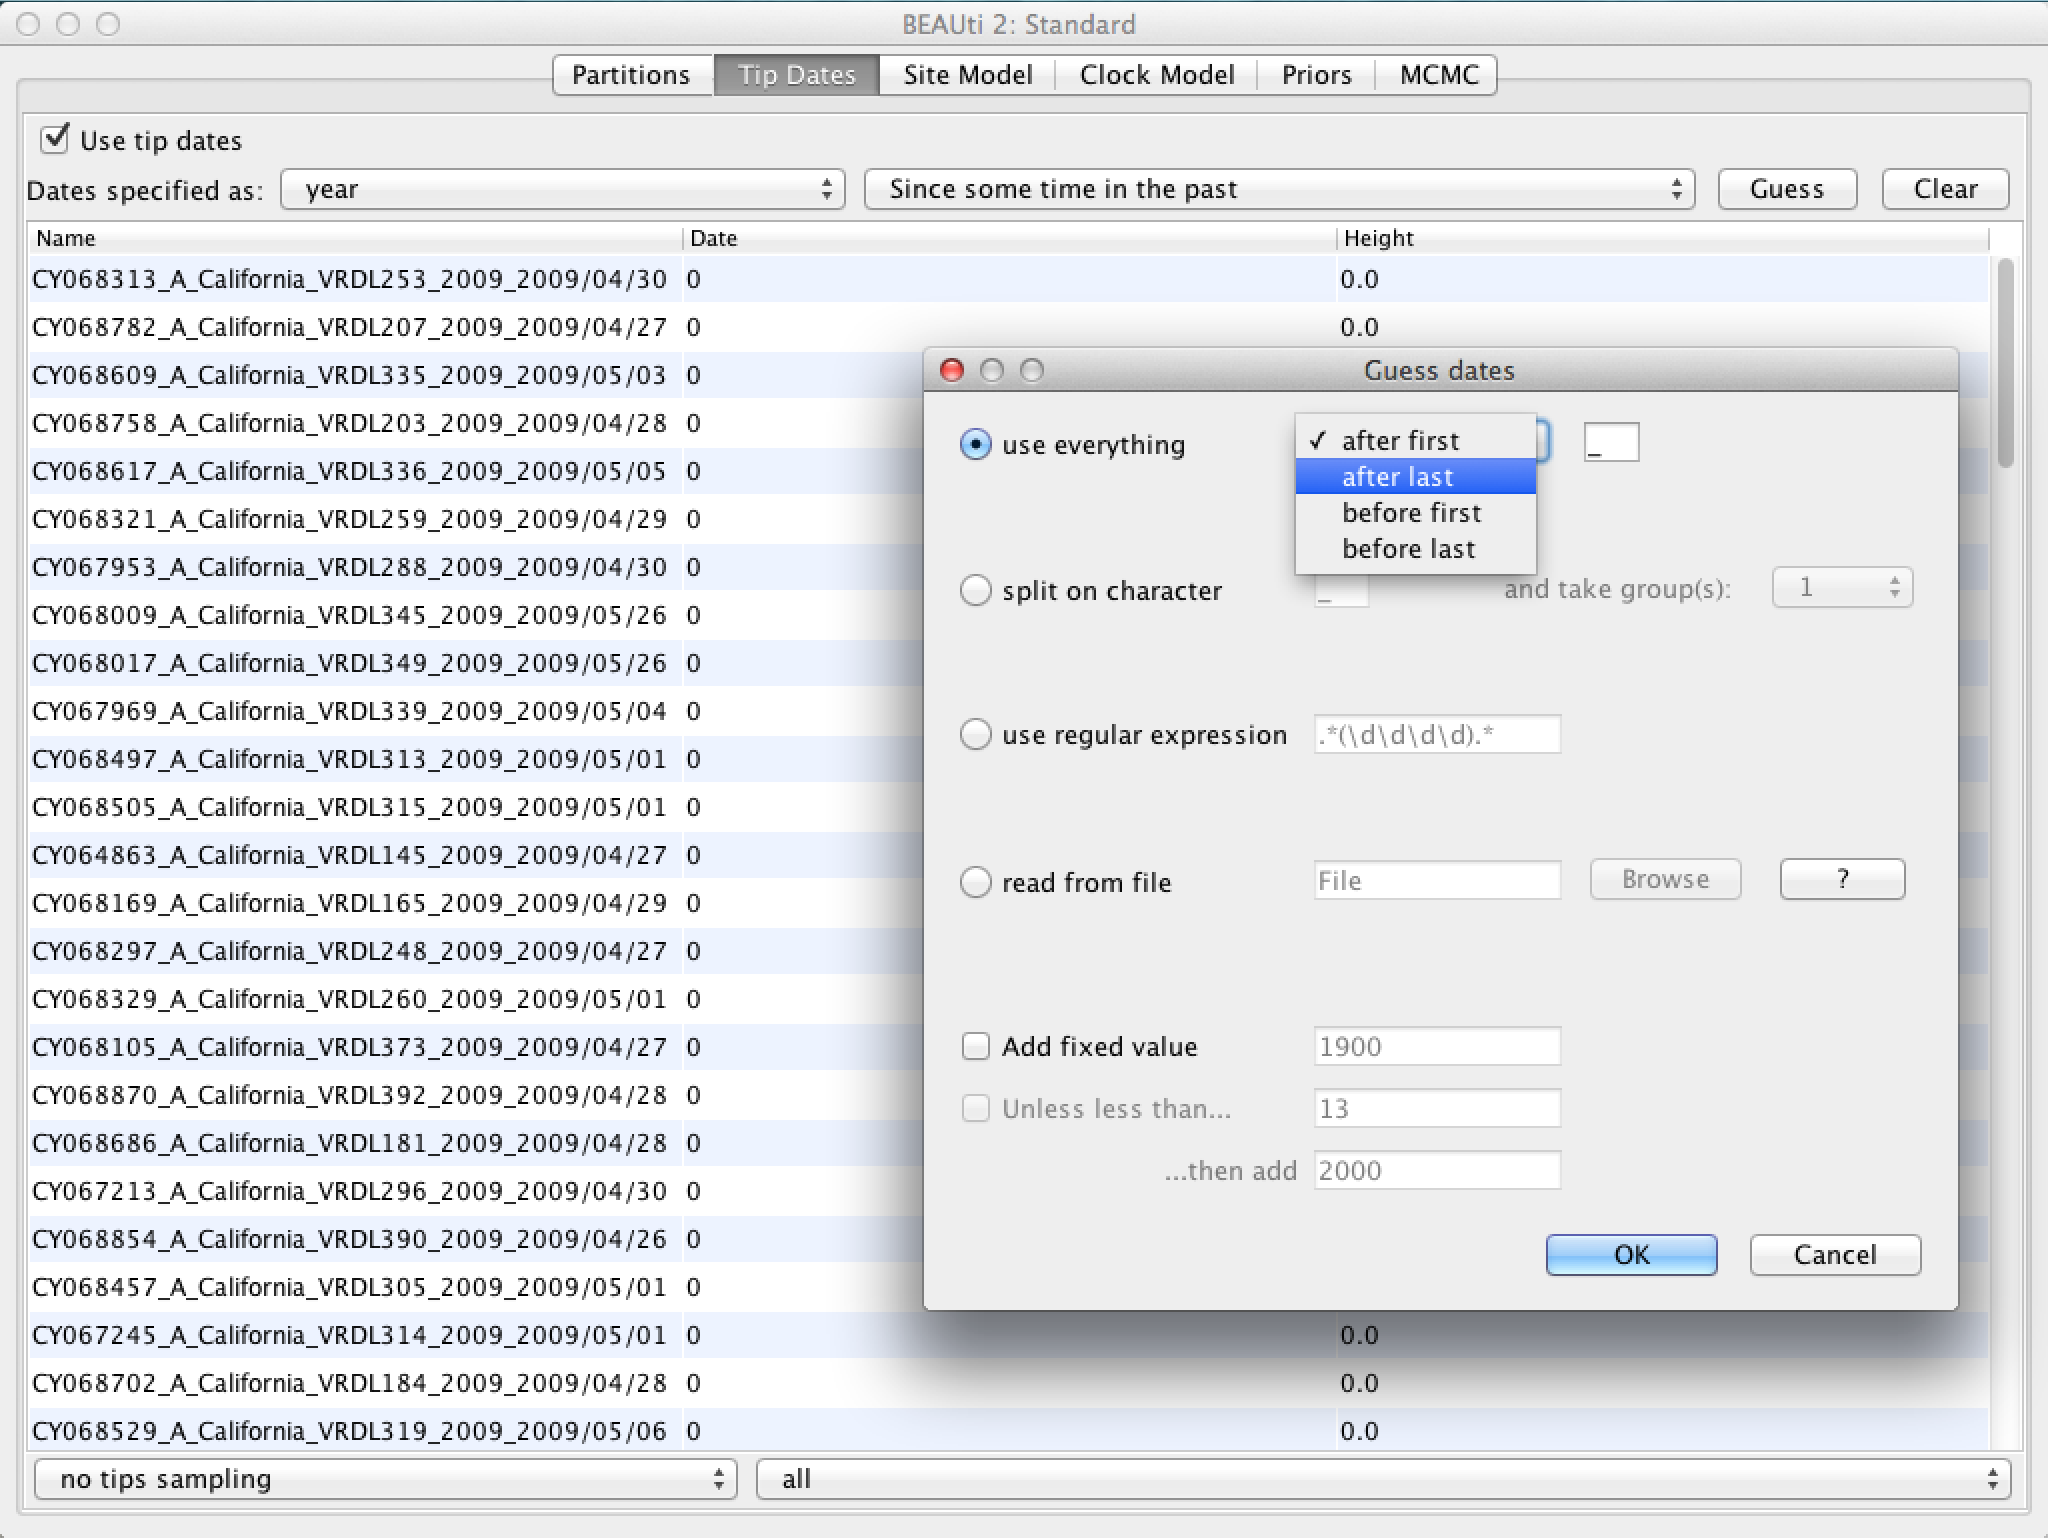
\includegraphics[width=0.75\textwidth]{figures/beast2_guess_dates.png}}
\caption{\small Specifying tip dates.}
\label{guessDates}
\end{figure}

You should now see that the tip ages have been filled in for all of the taxa and that the \textbf{Date} columns shows a number in form 2009.xyz and the \textbf{Height} column shows the number in form 0.abc (the height of the tip from present time, where present is 0.0).

Now we are done with the data specification and we are about to start specifying models and priors for the model parameters. 



\bigskip
\subsubsection{Specifying the Site Model}

\begin{framed}
Navigate to the \textbf{Site Model} panel, where we can choose the model of nucleotide evolution that we want to assume to underly our dataset. 
\end{framed}

Our dataset is made of nucleotide sequences. There are four models of nucleotide evolution available in BEAST2: JC69, HKY, TN93 and GTR. Most of these models were discussed in the lecture on substitution models. Remember that the JC69 model was the simplest evolutionary model. All the substitutions are assumed to happen with the same rate and all the bases are assumed to have identical frequencies, i.e. each base A, C, G and T is assumed to have equilibrium frequency of 0.25. In HKY model, the rate of transitions A$\leftrightarrow$G and C$\leftrightarrow$T is allowed to be different from the rate of transversions A$\leftrightarrow$C, G$\leftrightarrow$T. Furthermore, the frequency of each base can be either ``Estimated'', ``Empirical'' or ``All Equal''. When we set the frequencies to ``Estimated'', the frequency of each base will be co-estimated as a parameter during the BEAST run. If we use ``Empirical'', base frequencies will be set to the frequencies of each base found in the alignment. Finally, if set to ``All Equal'', the base frequencies will be set to 0.25. The TN93 model is slightly more complicated than HKY, by allowing for different rates of A$\leftrightarrow$G and C$\leftrightarrow$T transitions. Finally, the GTR model is the most general model, with 10 parameters (and can be re-parameterized to only contain 9 parameters). 

\begin{framed}
{\bf QUESTION: Which substitution model may be the most appropriate for our dataset and why?} 

You can discuss with your neighbour or with the teaching assistants if you like. After you have made your decision, continue with the tutorial.
\end{framed}

Since we do not have any extra information on how the data evolved, the decision is not clear cut. The best would be to have some independent information on what model fits the influenza data the best. Alternatively, one could perform model comparison, or apply reversible jump MCMC (see e.g. bModelTest, or substBMA)  to choose the best model. Let's assume, we have done some independent data analyses and found the HKY model to fit the influenza data the best. In general, this model captures the major biases that can arise in the analysis of the nucleotide data. 
%However, we have enough data to avoid using the simplest model (JC69) which is parametrised with just a single parameter. We also do not want to over-parametrize the model and so we choose the HKY model. This one takes into account the possibility that the transition rate may differ from the transversion rate. You could as well choose TN93 model, which has only one extra parameter as compared to HKY. 

Now we have to decide whether we want to assume all of the sites to have been subject to the same substitution rate or if we want to allow for the possibility that some sites were evolving faster than others. For this, we choose the number of gamma rate categories. Remember from the lecture on substitution models, that we basically scale the substitution rate by a factor, which is defined by our Gamma distribution. If we choose to split the Gamma distribution into 4 categories, we will have 4 scalings that will be applied to the substitution rate. The probability of substitution at each site will be calculated under each scaled substitution rate (and corresponding transition probability matrix) and averaged over the 4 outcomes.
  
\begin{framed}
{\bf QUESTION: Do you think a model that assumes one rate for all the sites is preferable over a model which allows different substitution rates across sites (i.e. allow for several gamma rate categories)? Why or why not?} 

You can again discuss with your neighbour or with the teaching assistants if you like. After you have made your decision, continue with the tutorial.
\end{framed}

Once again, a proper model comparison, i.e. comparing a model with no to a model with some number of gamma rate categories, would ideally be done. We do not have any independent information on whether gamma rate categories are needed or not. Thus, we take our best guess in order not to bias our analyses. Since the data are the sequences of the HA (hemagglutinin) gene of influenza, we may want to allow for variation of the substitution rates between sites. Hemagglutinin is a surface protein on the virus and is under significant evolutionary pressure from the immune system of the host organism. It is not unrealistic to assume that some sites may be under more pressure to escape from the immune system.

Let us therefore choose the HKY model with 4 gamma rate categories for the substitution rate. 

\begin{framed}
Change the \textbf{Gamma Category Count} to 4, tick the estimate box next to the \textbf{Shape} parameter of the Gamma distribution and set the \textbf{Subst Model} to \textbf{HKY}. [Figure \ref{substitutionModel}] 
\end{framed}

\begin{figure}[h!]
\centering
\fbox{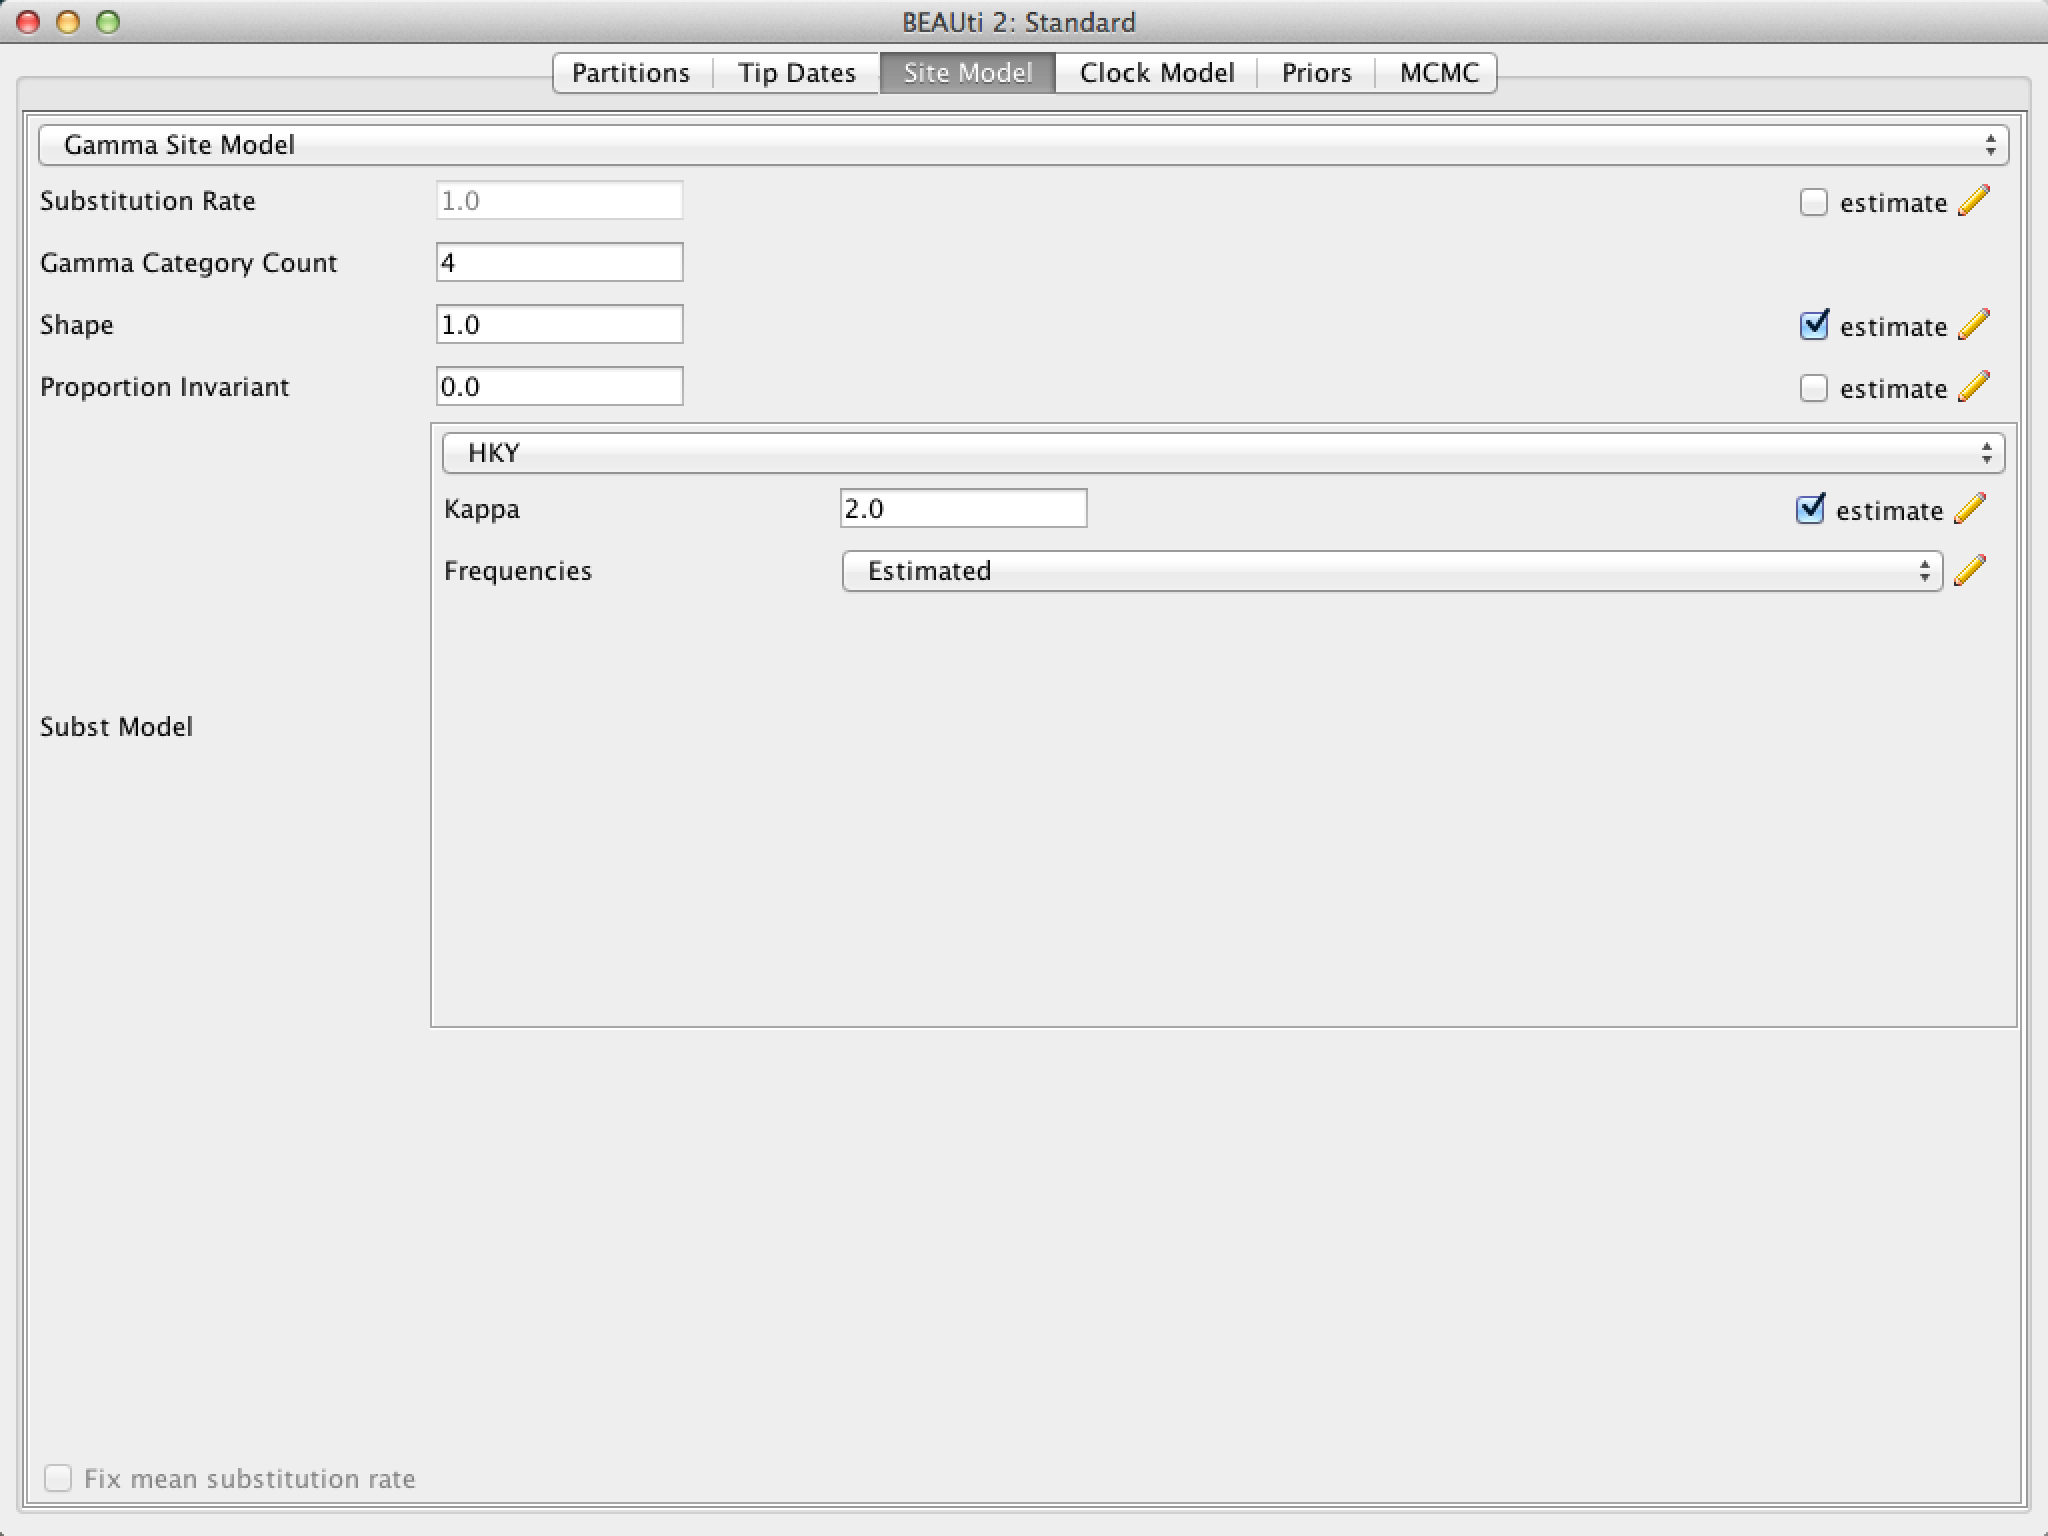
\includegraphics[width=0.75\textwidth]{figures/beast2_substitution_model.png}}
\caption{\small Specifying substitution model.}
\label{substitutionModel}
\end{figure}

Notice, that we estimate the shape parameter of the Gamma distribution as well. This is generally recommended, unless one is sure that the Gamma distribution with the shape parameter equal to 1 captures exactly the rate variation in the given dataset.
Notice also, that we leave the substitution rate fixed to 1.0 and do not estimate it. In fact, the overall substitution rate is the product of the clock rate and the substitution rate (one of the two acting as a scalar rather than a quantity measured in number of substitutions per site per time unit), and thus fixing one to 1.0 and estimating the other one allows for estimation of the overall rate of substitution. We will therefore use the clock rate to estimate the number of substitutions per site per year. 



\bigskip
\subsubsection{Specifying the Clock Model}

\begin{framed}
Navigate to the \textbf{Clock Model} panel.
\end{framed}

Four different clock models are available in BEAST 2, allowing us to specify lineage-specific substitution rate variation. The default model in BEAUti is the \textbf{Strict Clock} with a fixed substitution rate equal to 1. The other three models relax the assumption of a constant substitution rate. The \textbf{Relaxed Clock Log Normal} allows for the substitution rates associated with each branch to be independently drawn from a single, discretized log normal distribution (\cite{drummond06}). Under the \textbf{Relaxed Clock Exponential} model, the rates associated with each branch are drawn from an exponential distribution (\cite{drummond06}). Both of these models are uncorrelated relaxed clock models. The log normal distribution has the advantage that one can estimate its variance, which reflects the extent to which the molecular clock needs to be relaxed. In both models, BEAUti sets by default the \textbf{Number Of Discrete Rates} to -1. This means that the number of bins that the distribution is divided into is equal to the number of branches. The last available model is the \textbf{Random Local Clock} which averages over all possible local clock models (\cite{drummond10}). 

\begin{framed}
{\bf QUESTION: Which clock model may be the most appropriate for our dataset and why?} 
\end{framed}

Since we are observing the sequence data from a single epidemic of H3N2 virus in humans in a single location (south-west of USA), we do not have a reason to assume different substitution rates for different lineages. Thus, the most straightforward option is to choose the default \textbf{Strict Clock} model [Figure \ref{clockModel}]. Note however, that a rigorous model comparison would be the best way to proceed with the choice of the clock model.

\begin{figure}[h!]
\centering
\fbox{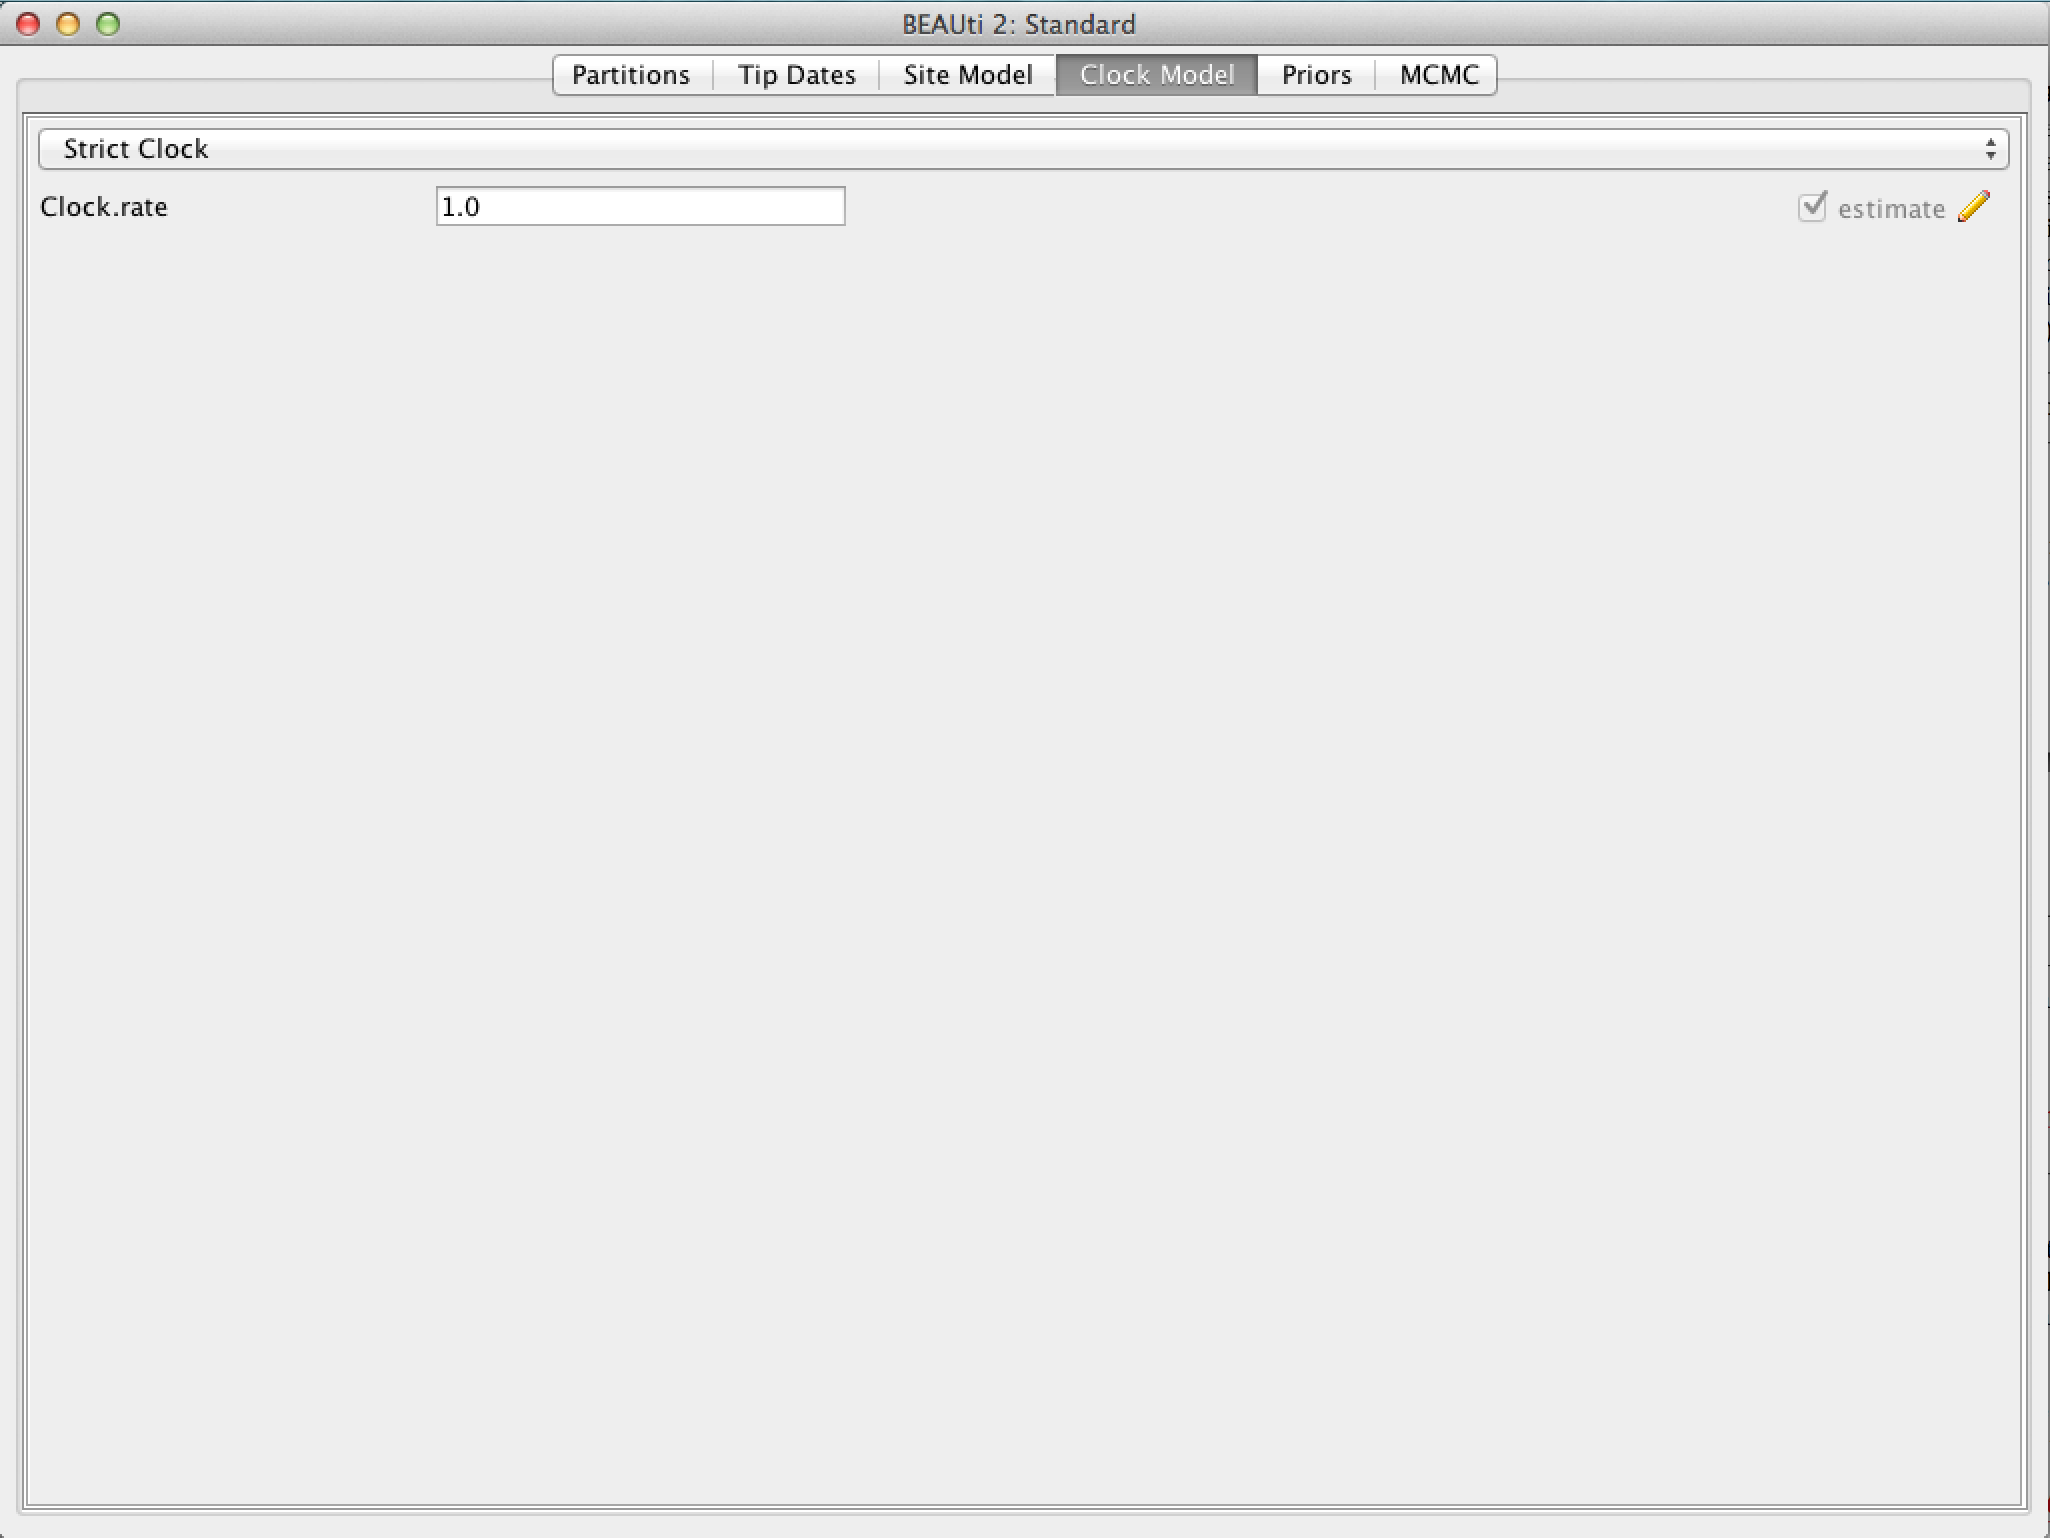
\includegraphics[width=0.75\textwidth]{figures/beast2_clock_model.png}}
\caption{\small Specifying the clock model.}
\label{clockModel}
\end{figure}



\bigskip
\subsubsection{Selecting Priors}

\begin{framed}
Navigate to the \textbf{Priors} panel.
\end{framed}

%What prior would you set for the dimension? We know the influenza epidemic starts up with one infection, rapidly increases in number of infecteds to eventually decline. 1 dimension is not sufficient. 

Since the dynamics of influenza virus is likely to change due to the depletion of susceptible population and/or presence of the resistant individuals, we choose the birth-death skyline model of population dynamics with 5 time intervals for R0, to capture this likely change of dynamics over time. R0, called basic reproductive number, is the ratio of the birth (or speciation) rate and the death (or extinction) rate. It is an important variable for the study of infectious diseases, since it defines how many individuals can get infected from a single infected individual in a completely susceptible population in the course of his/her infection. In other words, it tells us how quickly is the disease spreading in a population. R0 for any infection is very rarely above 10, so we set this as the upper value for R0 in our analysis.

\begin{framed}
For the \textbf{Tree} model, select the option \textbf{Birth Death Skyline Serial}. 

Then, click in the arrow to the left from \textbf{R0} to open all the options for R0 settings [Figure \ref{treePrior}]. Leave all the settings to the default, since it specifies not too strong prior on R0 around 1. This is exactly what we want. 

Then, click on the window where it says \textbf{initial = [2.0] [0.0, Infinity]}. A pop-up window will show up [Figure \ref{R0Prior}].

In the pop-up window change the \textbf{Upper}, the upper limit of the prior distribution, from Infinity to 10 and the \textbf{Dimension} of the R0 from 10 to 5 and click \textbf{OK}.
\end{framed}

\begin{figure}[h!]
\centering
\fbox{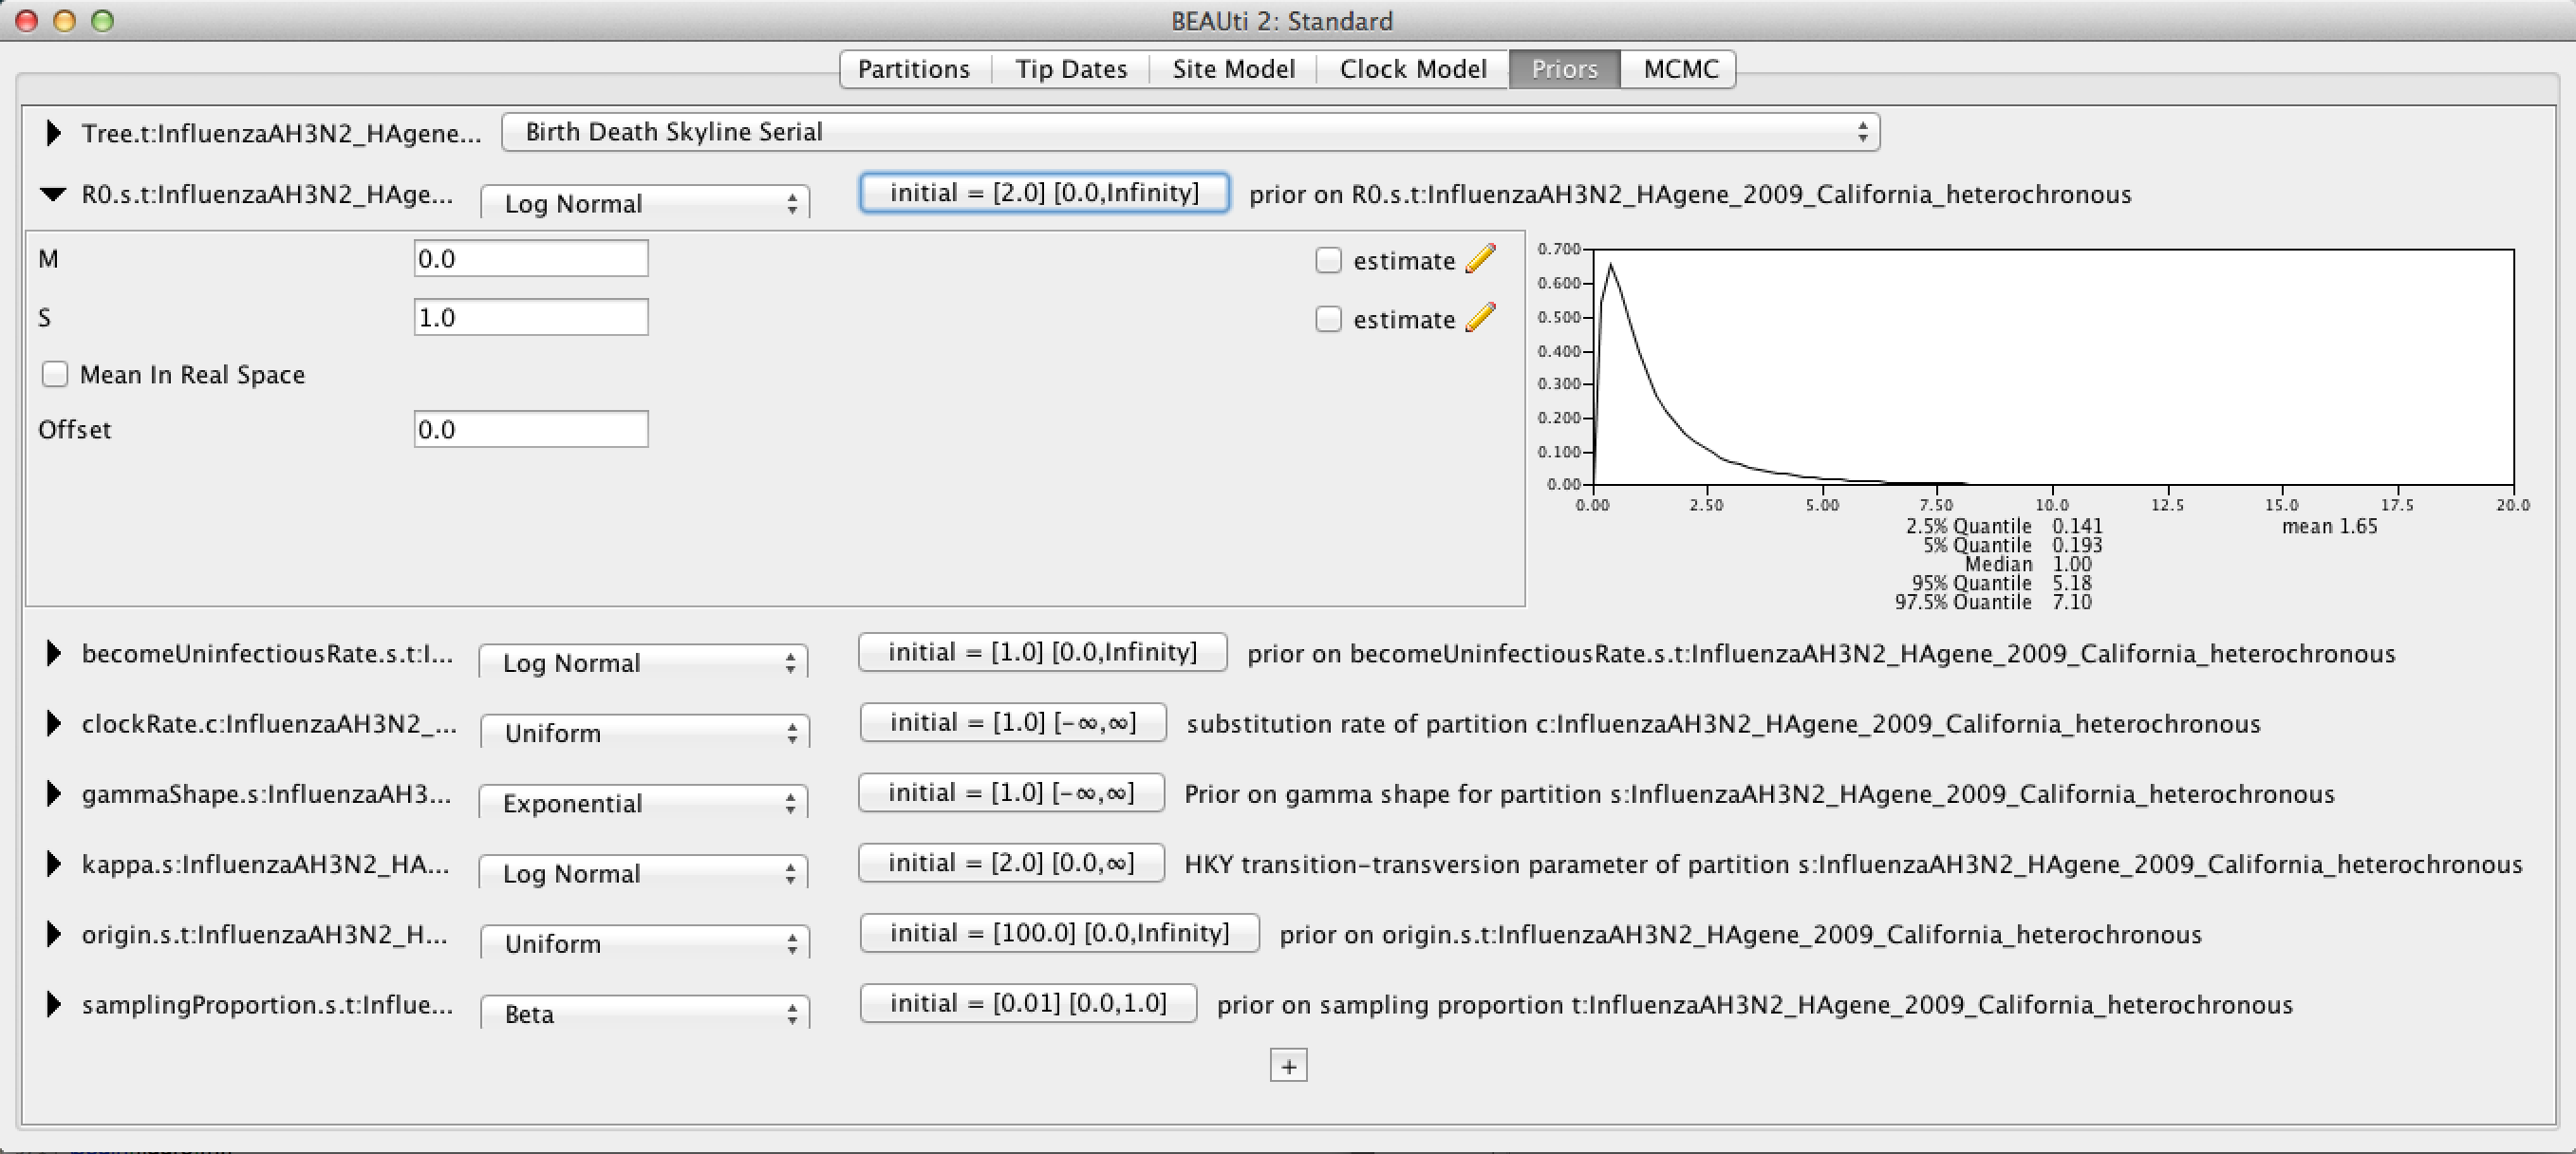
\includegraphics{figures/beast2_prior_R0.png}}
\caption{\small Specifying the tree prior.}
\label{treePrior}
\end{figure}

\begin{figure}[h!]
\centering
\fbox{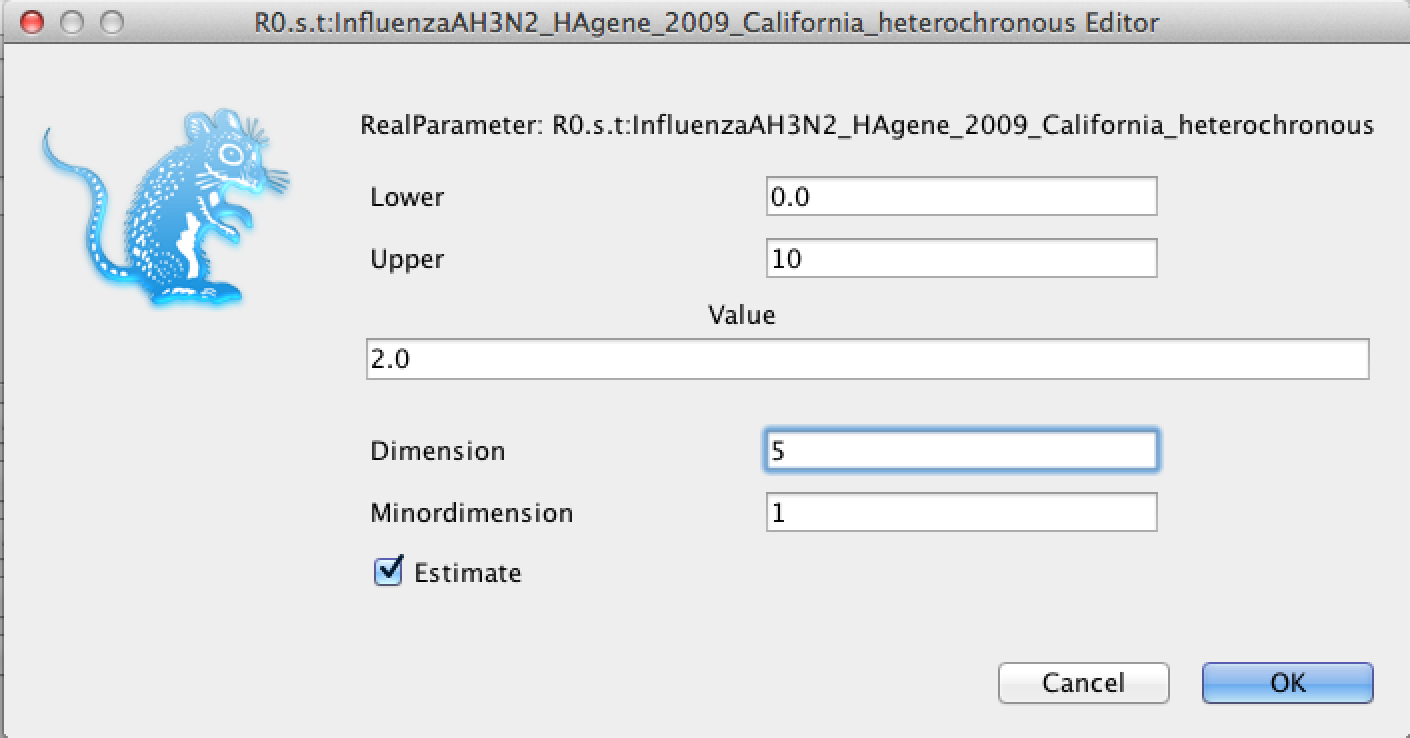
\includegraphics[width=0.5\textwidth]{figures/beast2_prior_R0dimension.png}}
\caption{\small Specifying the R0 prior.}
\label{R0Prior}
\end{figure}

Notice that the pop-up window allows one to specify not only the \textbf{Dimension} but also the \textbf{Minordimension}. If the parameter is specified as a vector of $n$ entries, we only use the \textbf{Dimension} with input $n$. If the parameter is specified as an n x m matrix, we then use the \textbf{Minordimension} to specify the number of columns (m) the parameter is split into. In the birth-death skyline model, we use the parameter vector only, and thus the \textbf{Minordimension} always stays specified as 1.

After we have specified the prior for R0, the next prior that needs our attention is the \textbf{becomeUninfectiousRate}. This specifies, how quickly does a person infected with influenza recover. From our personal experience, we would say, it takes around one week to 10 days from the infection of the person to the recovery. This translates to the become uninfectious rate of $365/10=36.5$ to $365/7\approx 52.14$ per year. Let us set the prior for become uninfectious rate accordingly.

\begin{framed}
 Click on the arrow next to the \textbf{becomeUninfectiousRate} and change the value for the \textbf{M} (mean) of the default log normal distribution to 52 and tick the box \textbf{Mean In Real Space} to specify the mean of the distribution in real space instead of a log space [Figure \ref{becomeUninfectiousPrior}].
\end{framed}

\begin{figure}[h!]
\centering
\fbox{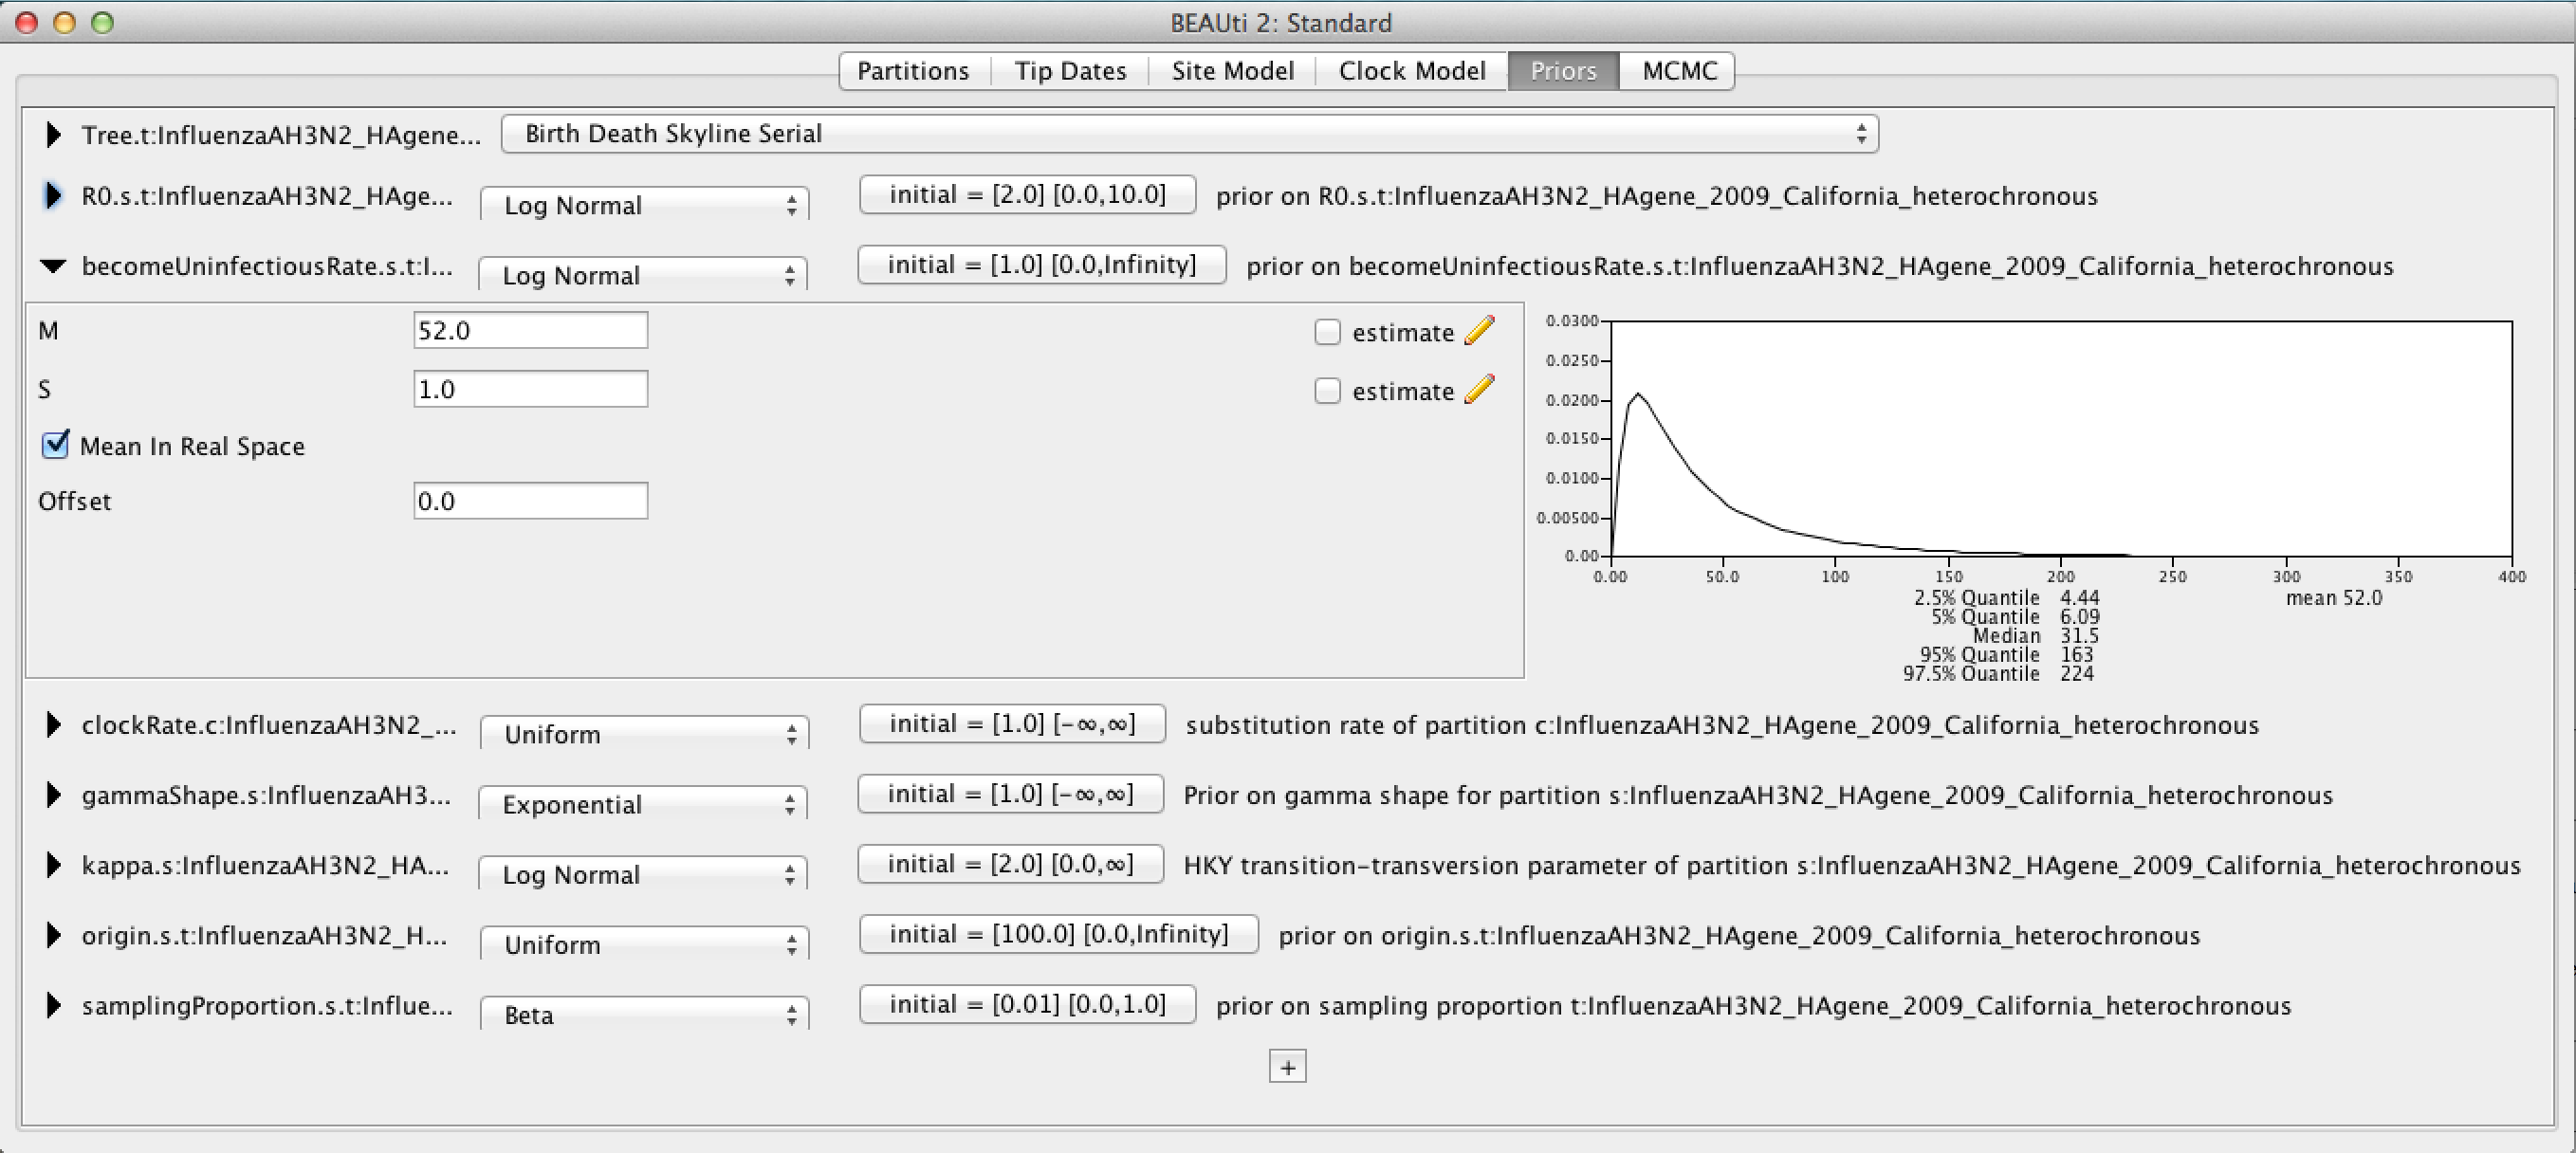
\includegraphics{figures/beast2_prior_becomeUninfectious.png}}
\caption{\small Specifying the become uninfectious prior.}
\label{becomeUninfectiousPrior}
\end{figure}

Now we have to specify the clock rate prior. This is basically the substitution rate prior.

\begin{framed}
{\bf QUESTION: What substitution rate is appropriate for viruses? More specifically, what substitution rate is expected for influenza virus, in your opinion?} 
\end{framed}

You could set your best guess as a prior, say, by choosing a log normal distribution centred around your best guess for the substitution rate. 

Now consider the following information: Influenza virus is an RNA virus \citep{kawaoka2006} and RNA viruses in general, have a mutation rate of $\approx 10^{-3}$ substitutions per site per year \citep{jenkins2002}. 

\begin{framed}
{\bf QUESTION: Did you change your best guess, for the substitution rate appropriate for RNA viruses? What would it be? How would you specify the prior?} 
\end{framed}
% For circulating influenza viruses in humans, which were under selection pressure, the fixation rates were estimated to be 3.7 * 10?3 and 5.72 * 10?3 nucleotide substitutions per site per year for the HA genes of influenza A(H3N2) viruses; these rates were based on the estimated accumulation of adaptive substitutions in human influenza A(H3N2) viruses during the periods 1983 to 1997 and 1992 to 2005, respectively (22, 23).
%Newly Emerging Mutations in the Matrix Genes of the Human Influenza A(H1N1)pdm09 and A(H3N2) Viruses Reduce the Detection Sensitivity of Real-Time Reverse Transcription-PCR

Our best guess would be to set the prior distribution peaked around $10^{-3}$ substitutions per site per year.

\begin{framed}
Click on the arrow next to the \textbf{clockRate} and change the value for the \textbf{M} (mean) of the default log normal distribution to 0.001 and tick the box \textbf{Mean In Real Space} [Figure \ref{clockRatePrior}].
\end{framed}

\begin{figure}[h!]
\centering
\fbox{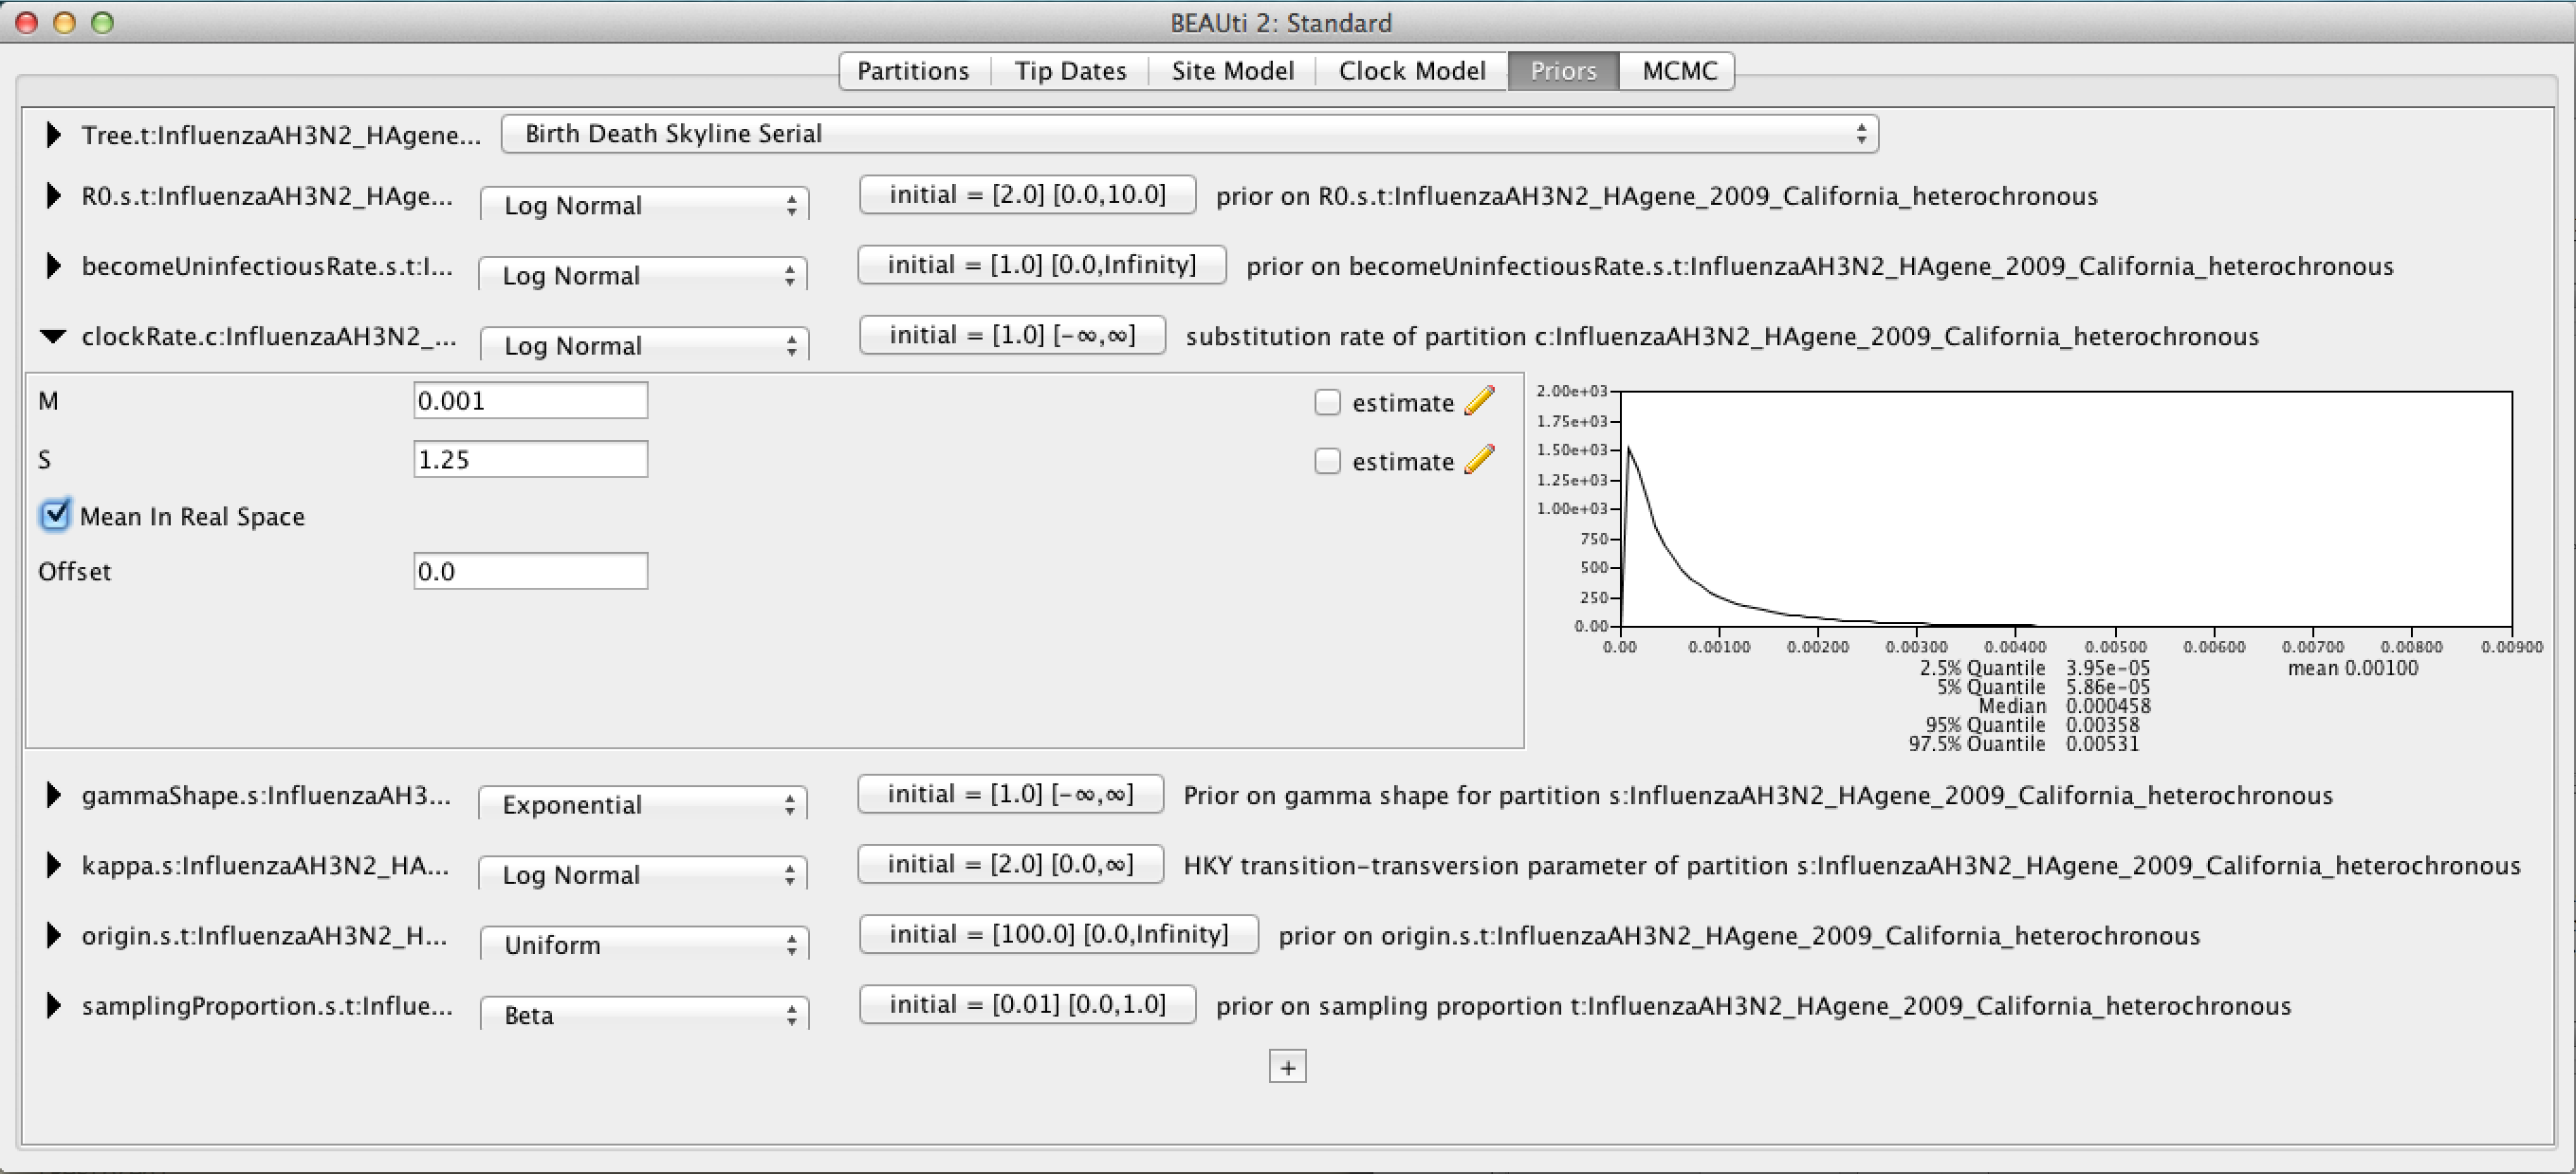
\includegraphics{figures/beast2_prior_clockRate.png}}
\caption{\small Specifying the clock rate prior.}
\label{clockRatePrior}
\end{figure}

%gamma shape parameter
We also need to estimate the gamma shape parameter, which governs the shape of the Gamma distribution of the rates across different sites. The setting alpha=beta=1.0 reflects our belief that on average, the rate scaler is equal to 1, i.e. on average all the sites mutate with the same substitution rate. The distribution on the gamma shape parameter allows us to deviate from this assumption. The default exponential distribution with M (mean) of 1.0 and 95\%HPD of [0.0253,3.69] covers a wide range of possible shape parameters. This looks fine for our analysis, and thus, we leave the gamma shape settings at its defaults [Figure \ref{gammaShapeprior}].
 
\begin{figure}[h!]
\centering
\fbox{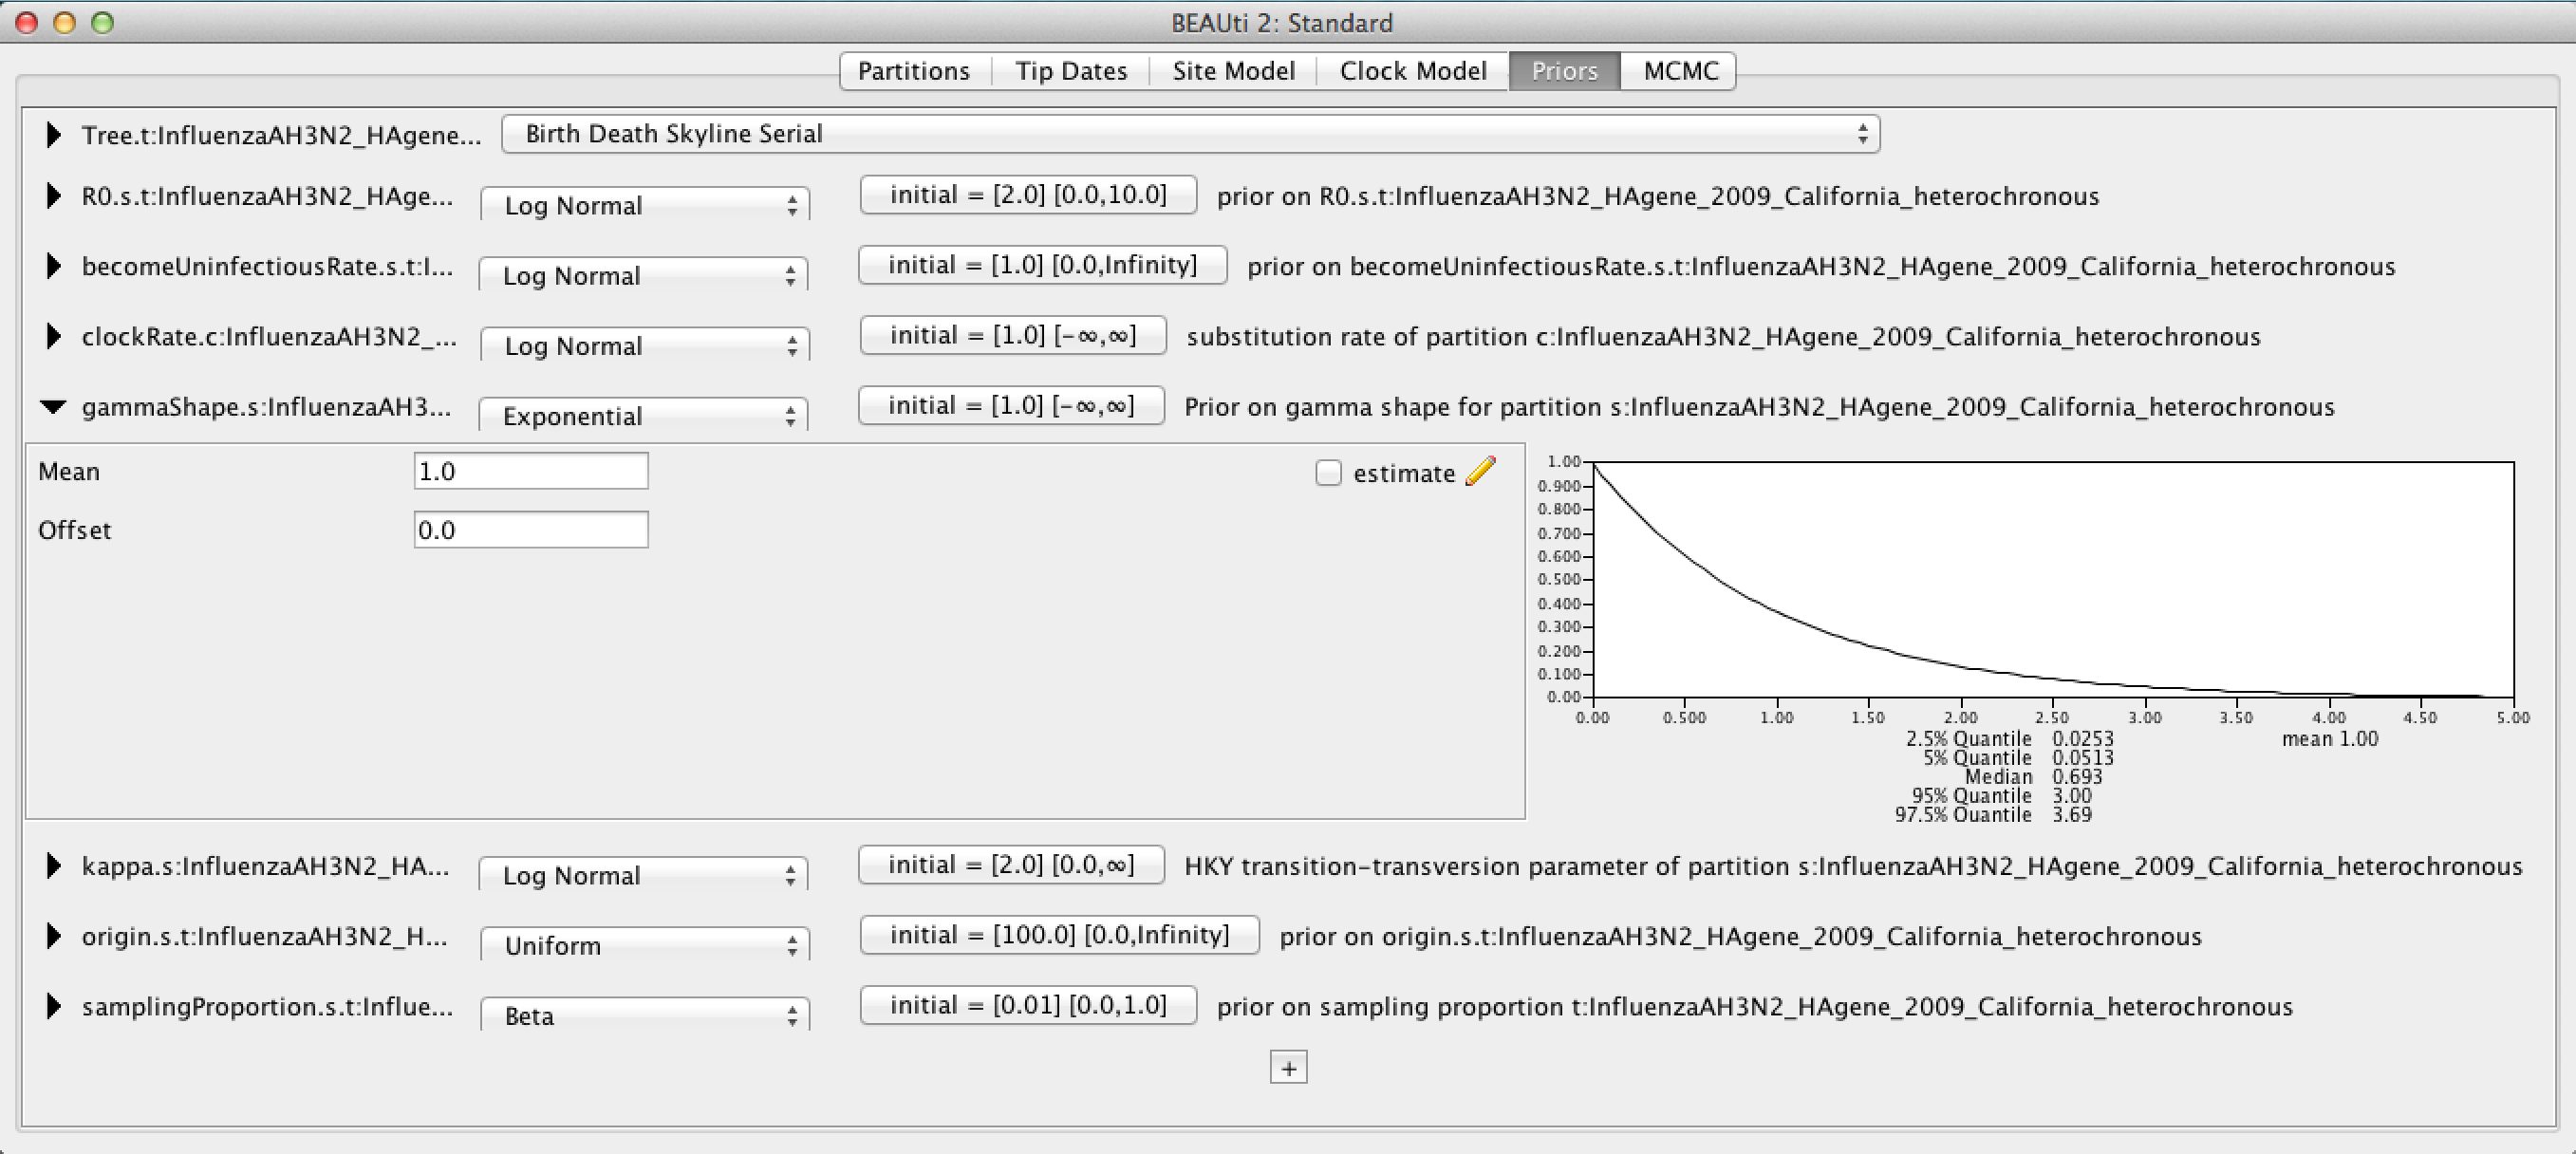
\includegraphics{figures/beast2_prior_gammaShape.png}}
\caption{\small Specifying the gamma shape prior.}
\label{gammaShapeprior}
\end{figure}

\newpage
%kappa
We do not have any prior information on transition-transversion ratio besides the fact that it is a value usually larger than 1 (transitions are more frequent than transversions). We therefore set a weakly informative prior for this parameter. The default log normal prior perfectly fits to these requirements [Figure \ref{kappaPrior}]. 

\begin{figure}[h!]
\centering
\fbox{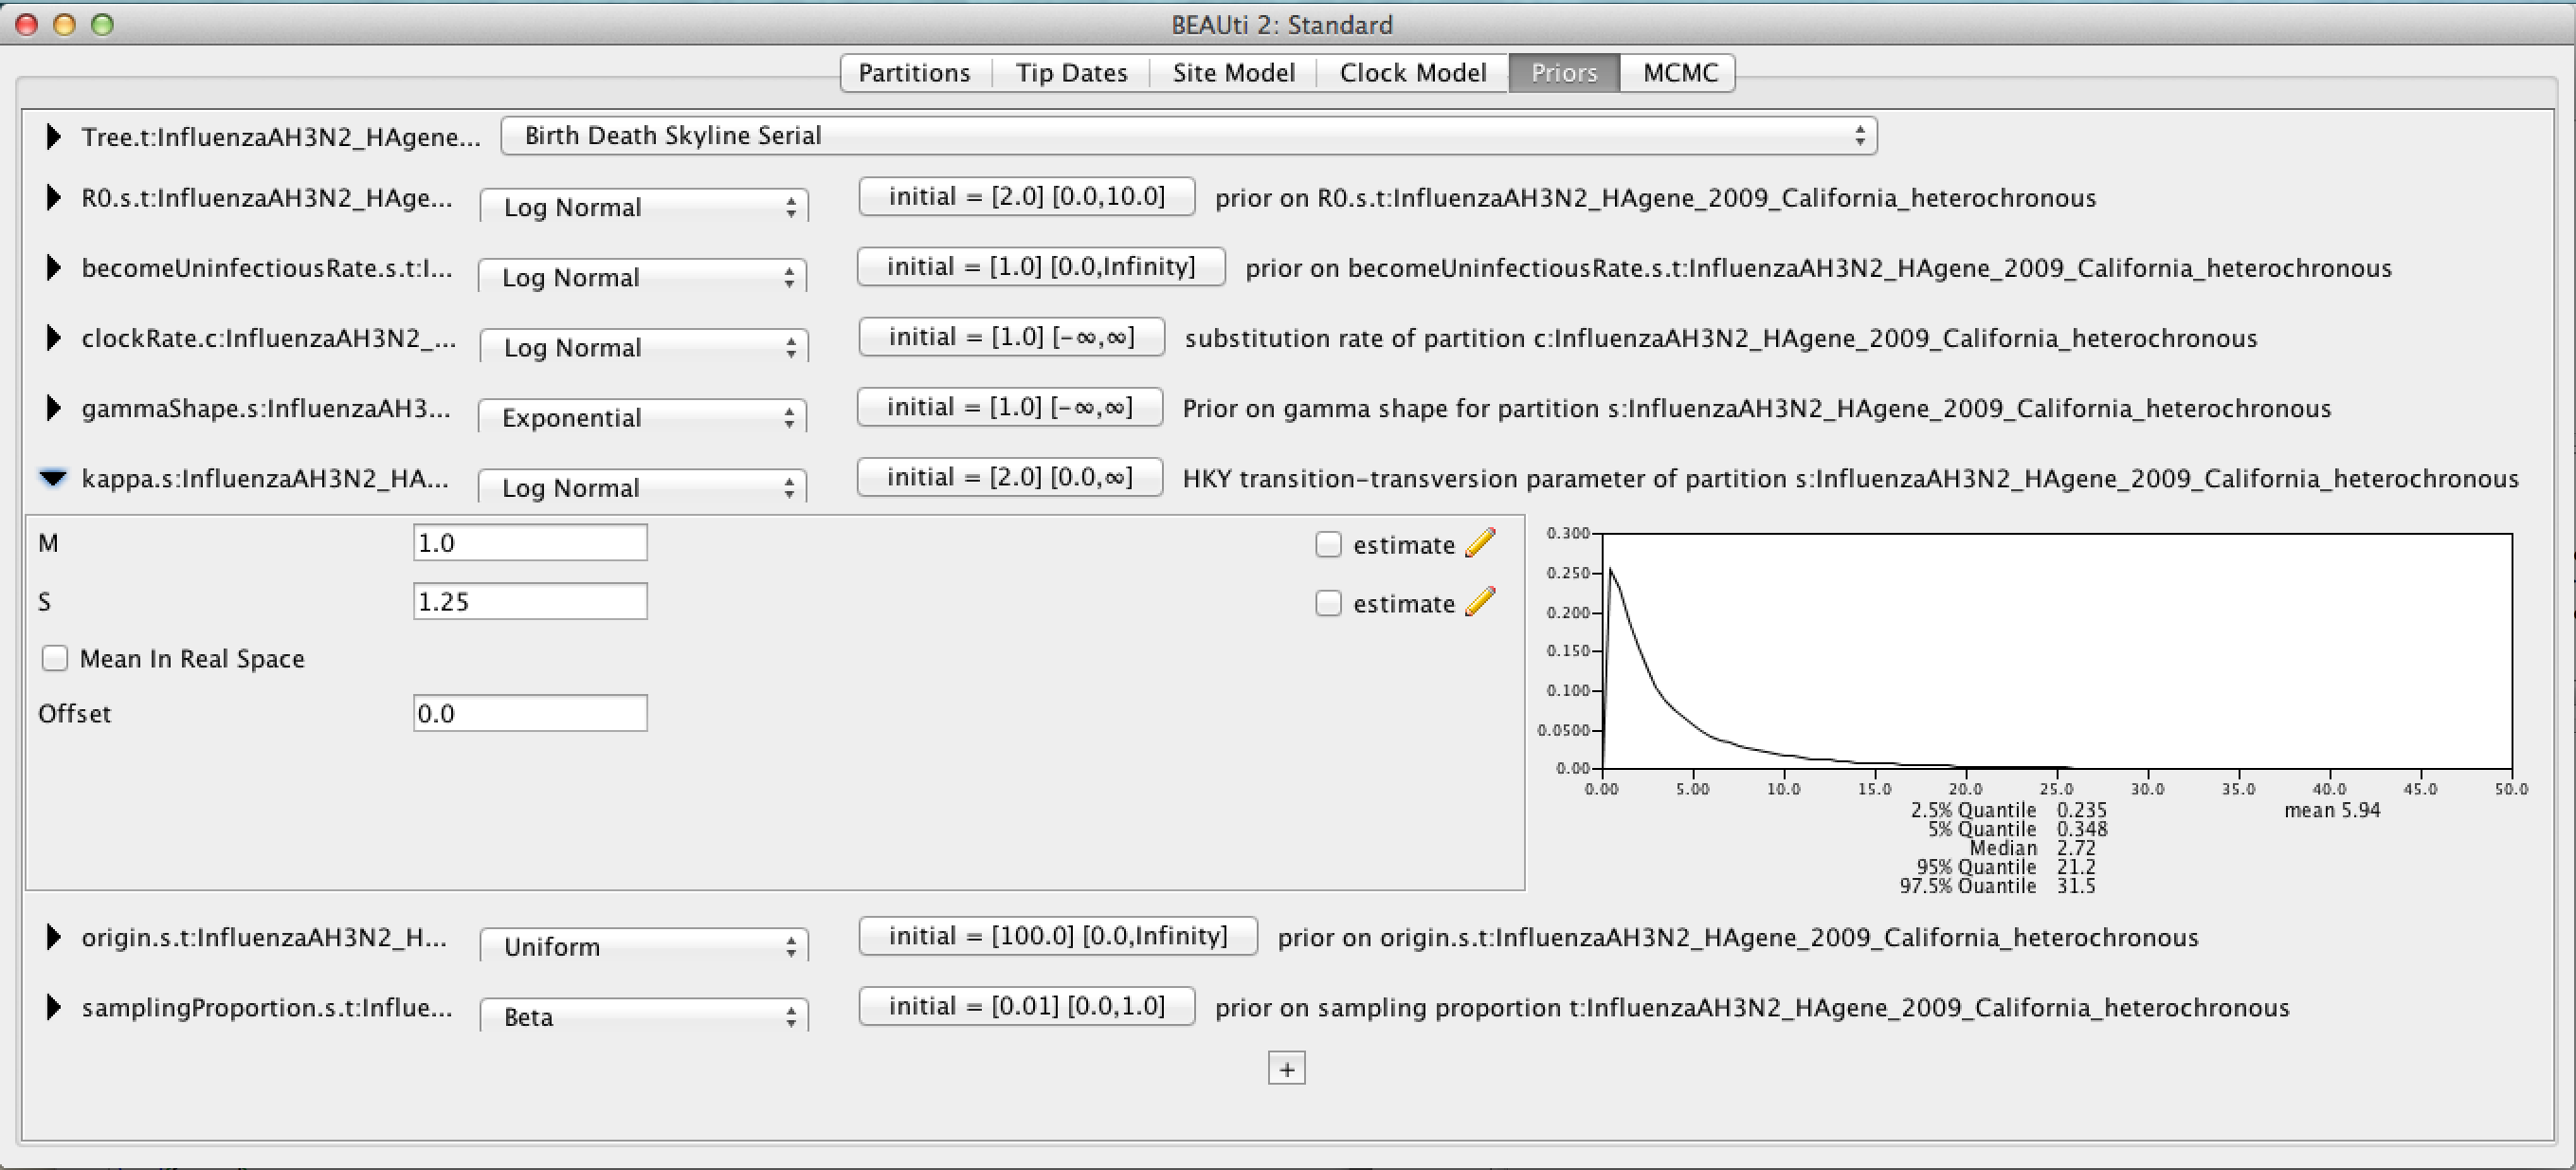
\includegraphics{figures/beast2_prior_kappa.png}}
\caption{\small Specifying the kappa (transition/transversion ratio) prior.}
\label{kappaPrior}
\end{figure}

%origin
For the next parameter, origin, we ask ourselves whether there is any reasonable expectation we might have in terms of when the infection in California started, i.e. what is the date when the ancestor of all of the sequences first appeared.

\begin{framed}
{\bf QUESTION: Do you have any feeling for what the origin should/could be set to?} 
\end{framed}

The data span a period of 3 months and are only coming from a limited area; thus, it would be unreasonable to assume that a single season flu epidemic would last longer than a few months. The best guess for the origin parameter prior we could make is  therefore on the order of at least 3-4, up to 6 months. We set the prior according to this expectation.

\begin{framed}
Click on the arrow next to the \textbf{origin} and change the prior distribution from \textbf{Uniform} to \textbf{Gamma} with Alpha parameter set to 0.5 and Beta parameter set to 2.0 [Figure \ref{originPrior}].
%
%Make sure that the \textbf{Lower} is set to 0.
\end{framed}

\begin{figure}[h!]
\centering
\fbox{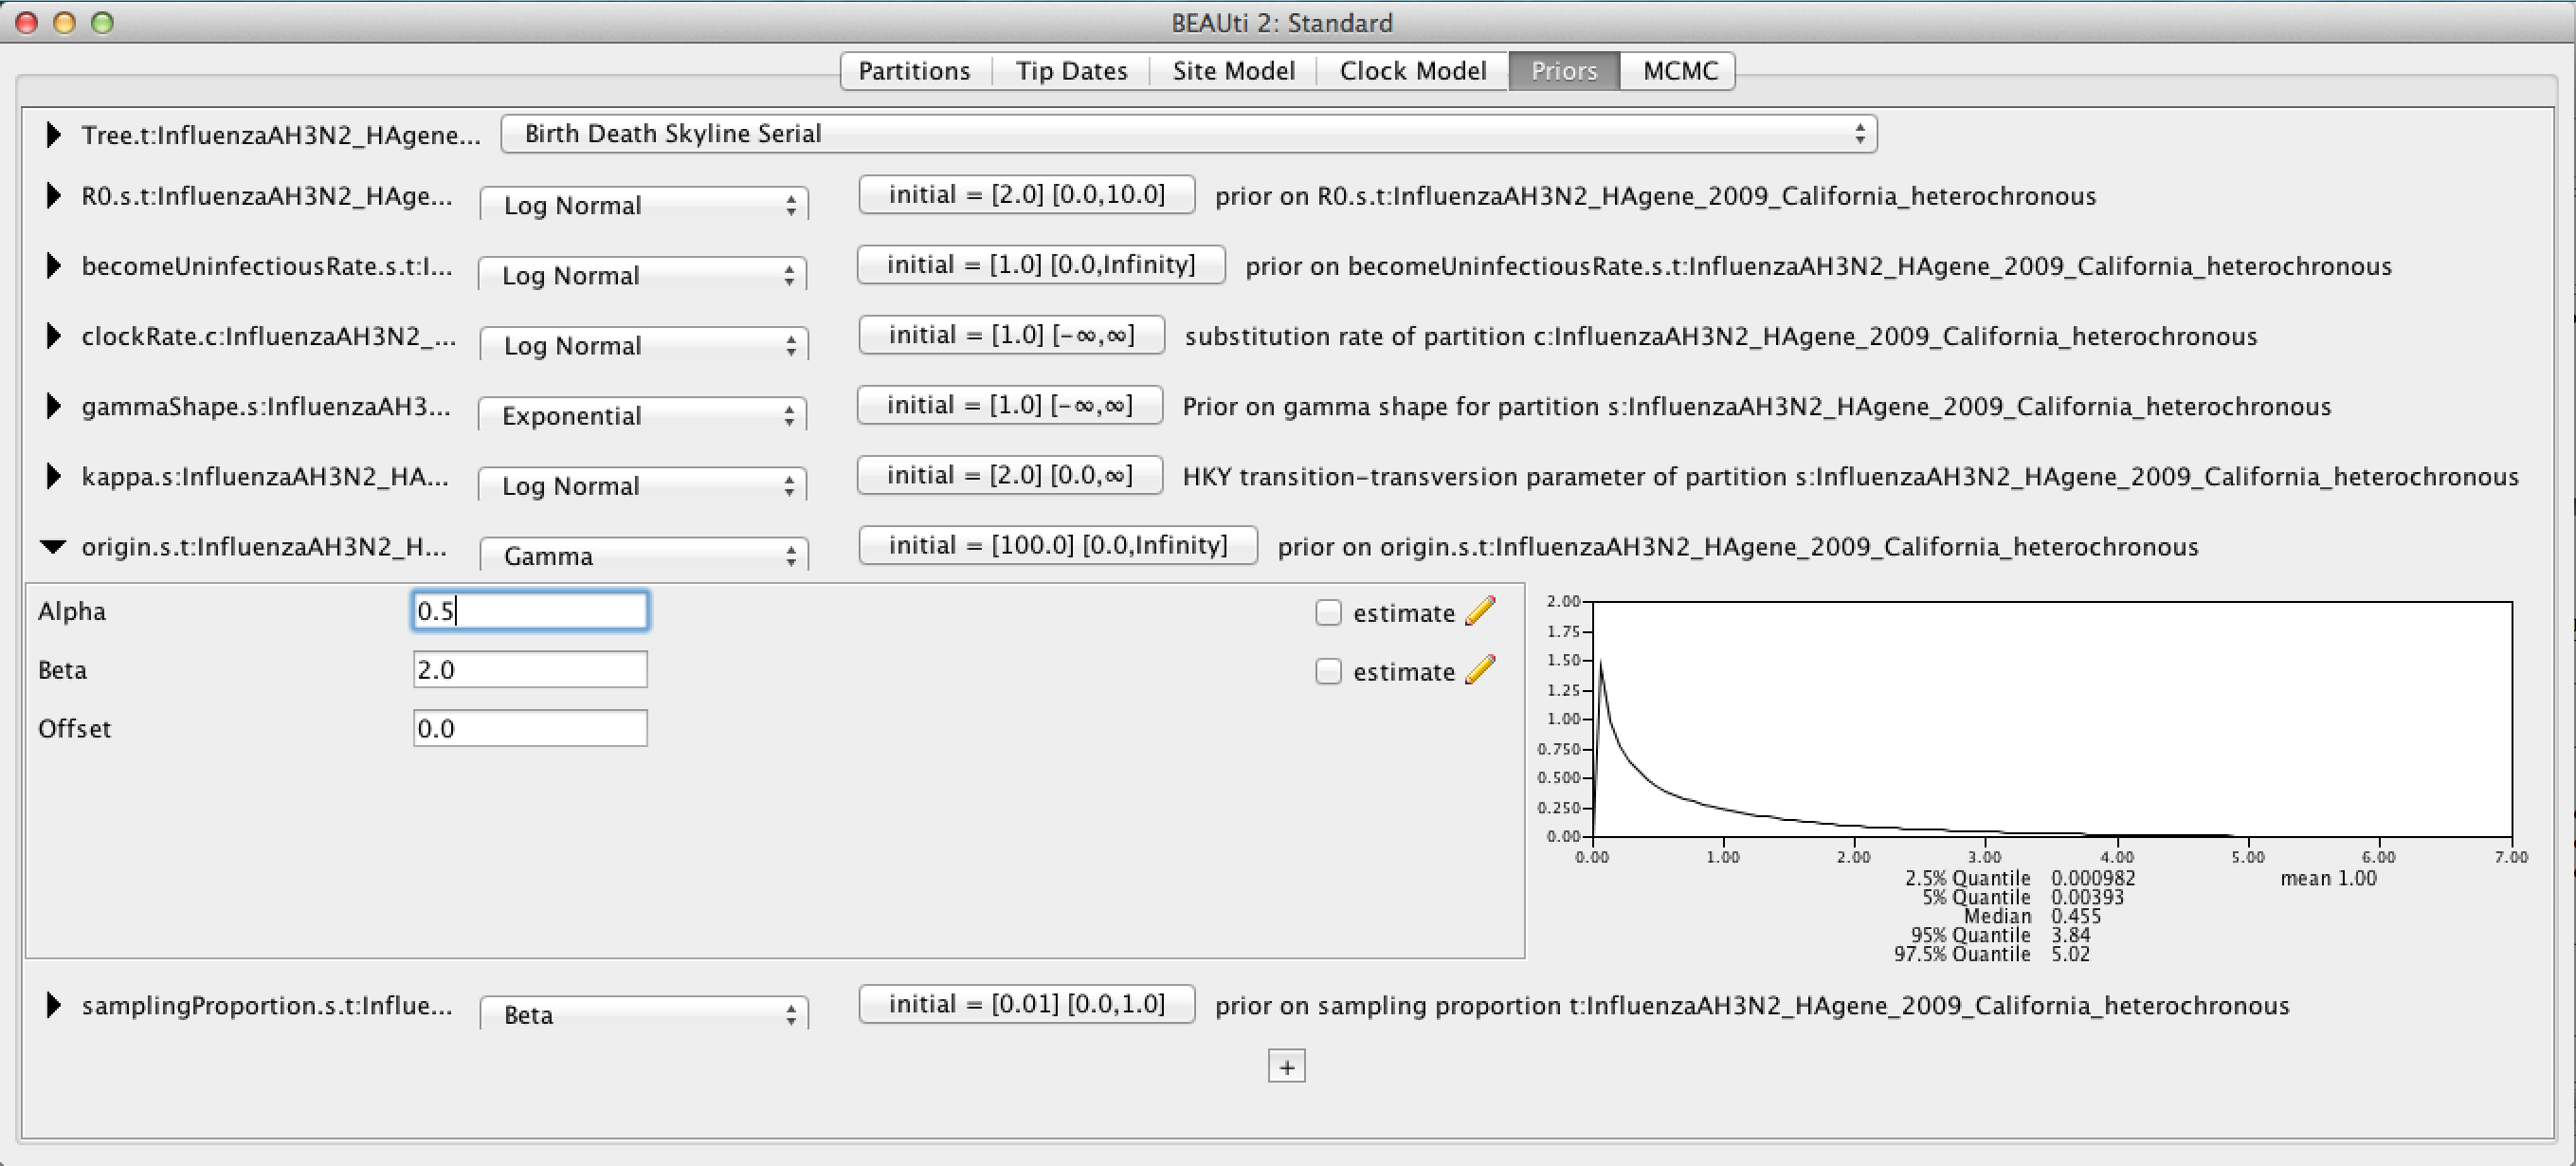
\includegraphics{figures/beast2_prior_origin.png}}
\caption{\small Specifying the origin prior.}
\label{originPrior}
\end{figure}

% If this is used, problems with initialisation
%\newpage
%Furthermore, the origin value that we expect is positive and most likely not larger than 1. We reflect this in the \textbf{origin} specification as follows:
%
%\begin{framed}
%Click on the window where it says \textbf{initial = [100.0] [0.0, Infinity]}. A pop-up window will show up [Figure \ref{originPriorPop}].
%
%In the pop-up window make sure that the \textbf{Lower}, the lower limit of the prior distribution is set to 0 (do not allow for negative values) and set the \textbf{Value} of the origin from 100.0 to 1.0 and click \textbf{OK}.
%\end{framed}
%
%\begin{figure}[h!]
%\centering
%\fbox{\includegraphics[width=0.5\textwidth]{figures/beast2_prior_originpop.png}}
%\caption{\small Specifying the origin lower limit and starting value.}
%\label{originPriorPop}
%\end{figure}

%sampling proportion
Lastly, for the sampling proportion, we know that we certainly did not sample every single infected individual. Therefore, setting a prior around 1 would not be reasonable. Actually, it is more reasonable to usually expect only a proportion of less than 0.1 of all flu cases to be sampled. Here, we specify something on the order of $10^{-3}$.

\begin{framed}
Click on the arrow next to the \textbf{samplingProportion} and change the distribution from \textbf{Beta} to \textbf{Log Normal}. 

Next, change the value for the \textbf{M} (mean) to 0.001 and tick the box \textbf{Mean In Real Space} [Figure \ref{samplingProportionPrior}].

Also, make sure that the \textbf{Lower} is set to 0.0 and the \textbf{Upper} is set to 1.0.
\end{framed}

\begin{figure}[h!]
\centering
\fbox{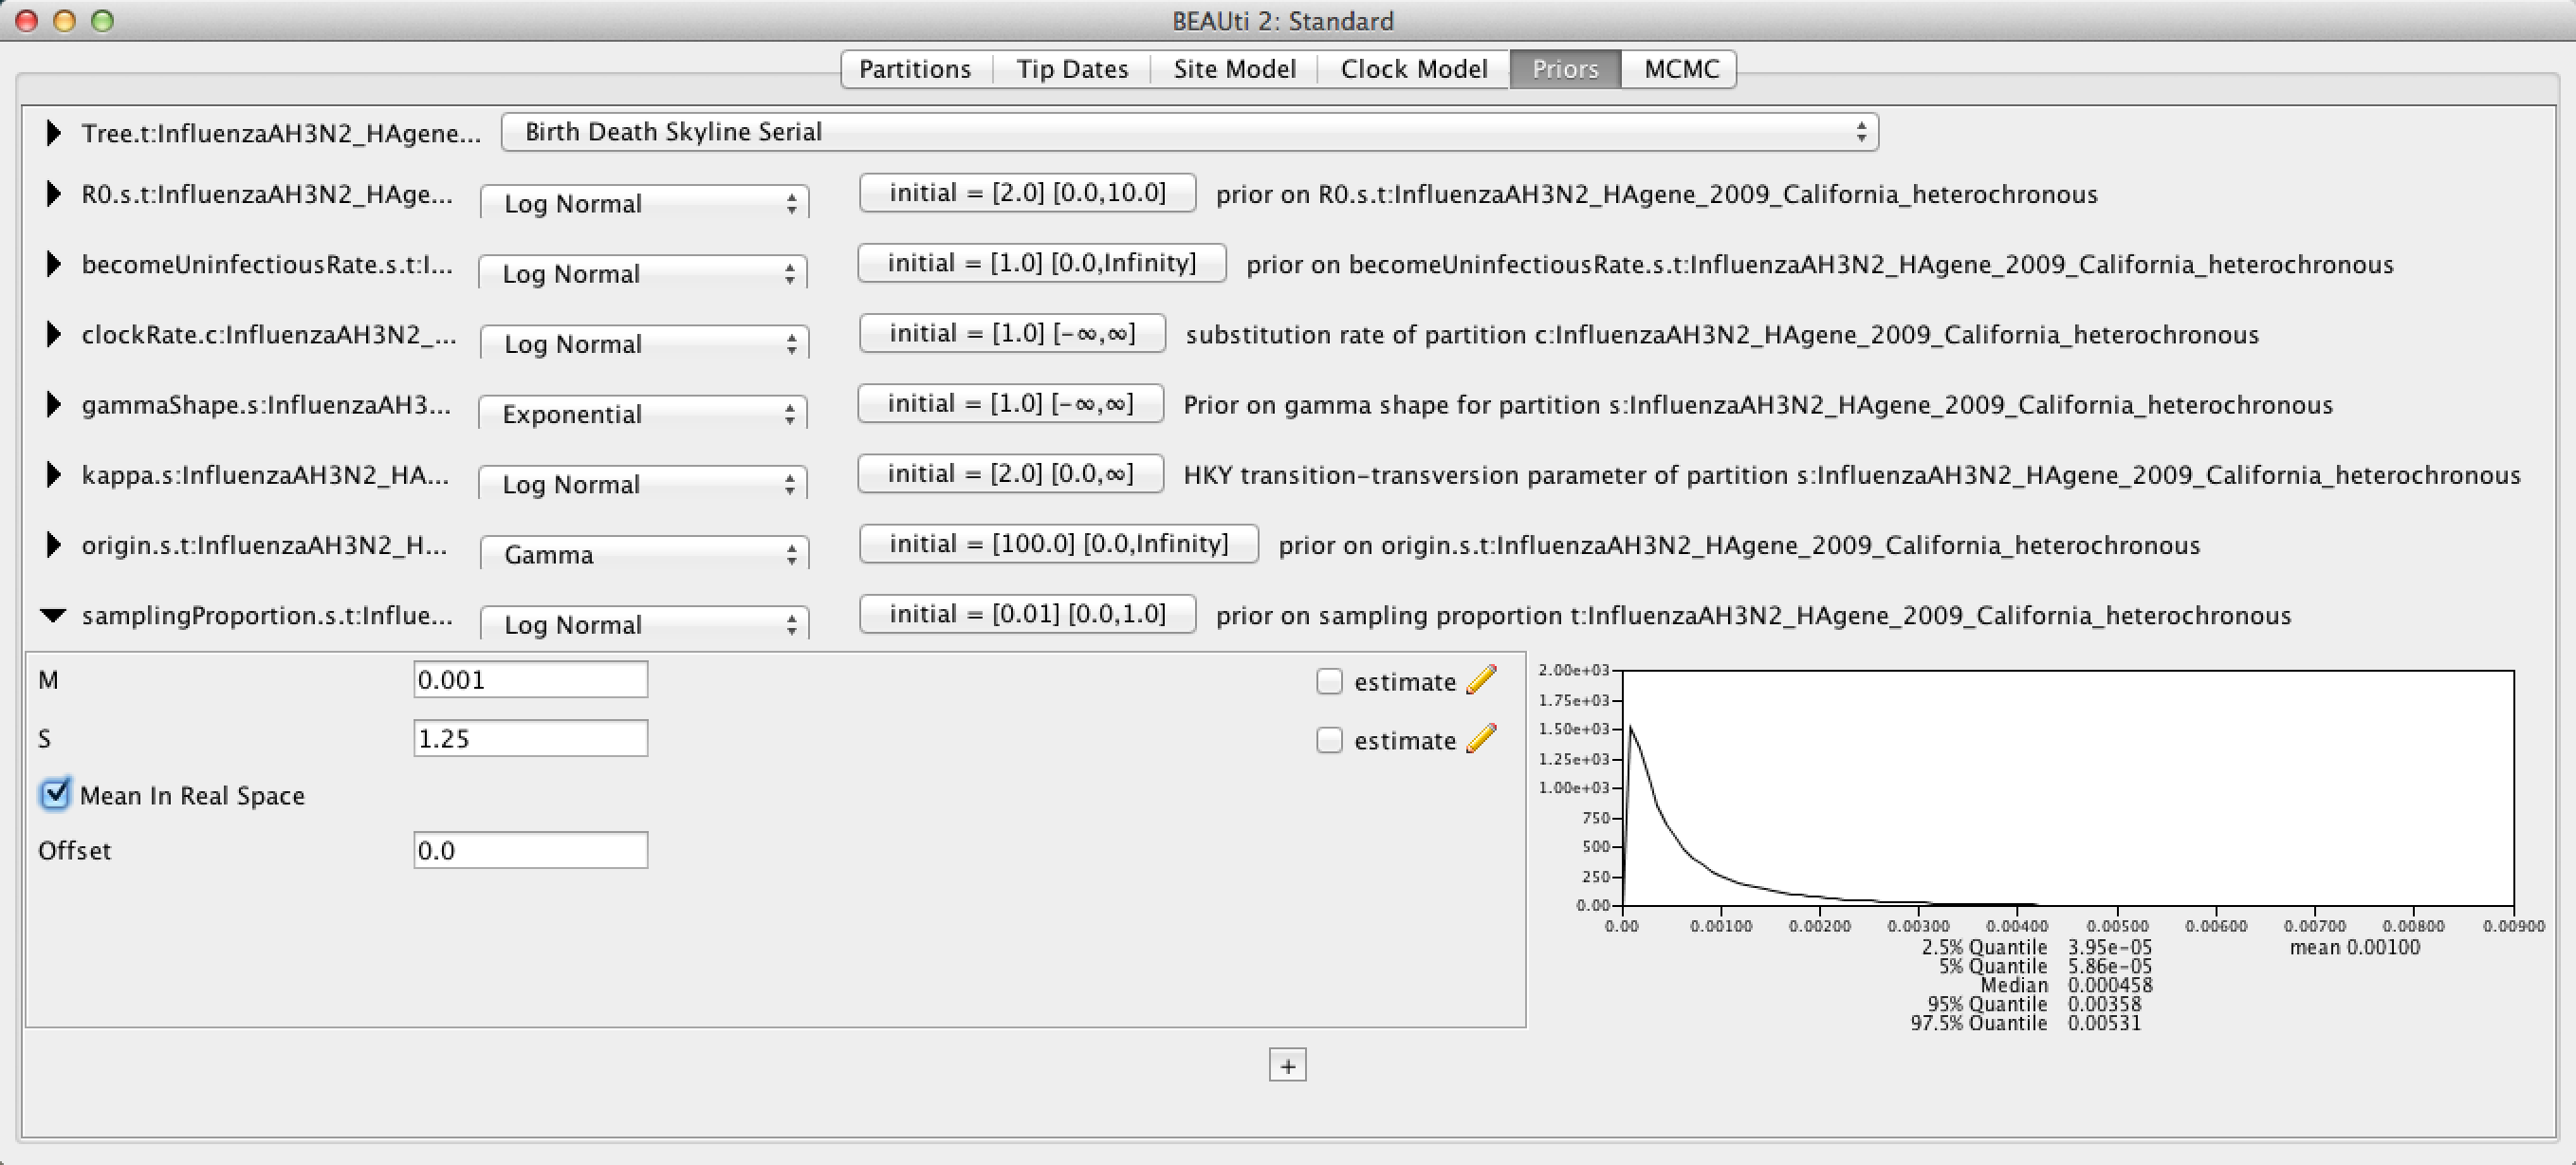
\includegraphics{figures/beast2_prior_samplingProportion.png}}
\caption{\small Specifying the sampling proportion prior.}
\label{samplingProportionPrior}
\end{figure}



\bigskip
\subsubsection{MCMC}

\begin{framed}
Navigate to the \textbf{MCMC} panel.
\end{framed}

We want to shorten the chain length, in order for it to run in a reasonable time and we want to decrease the tree sampling frequency.

\begin{framed}
Change the \textbf{Chain Length} from 10'000'000 to 5'000'000.

Click on the arrow next to the \textbf{tree log} and set the \textbf{Log Every} to 100'000 [Figure \ref{mcmc}].
\end{framed}

%mcmc chain
\begin{figure}[h!]
\centering
\fbox{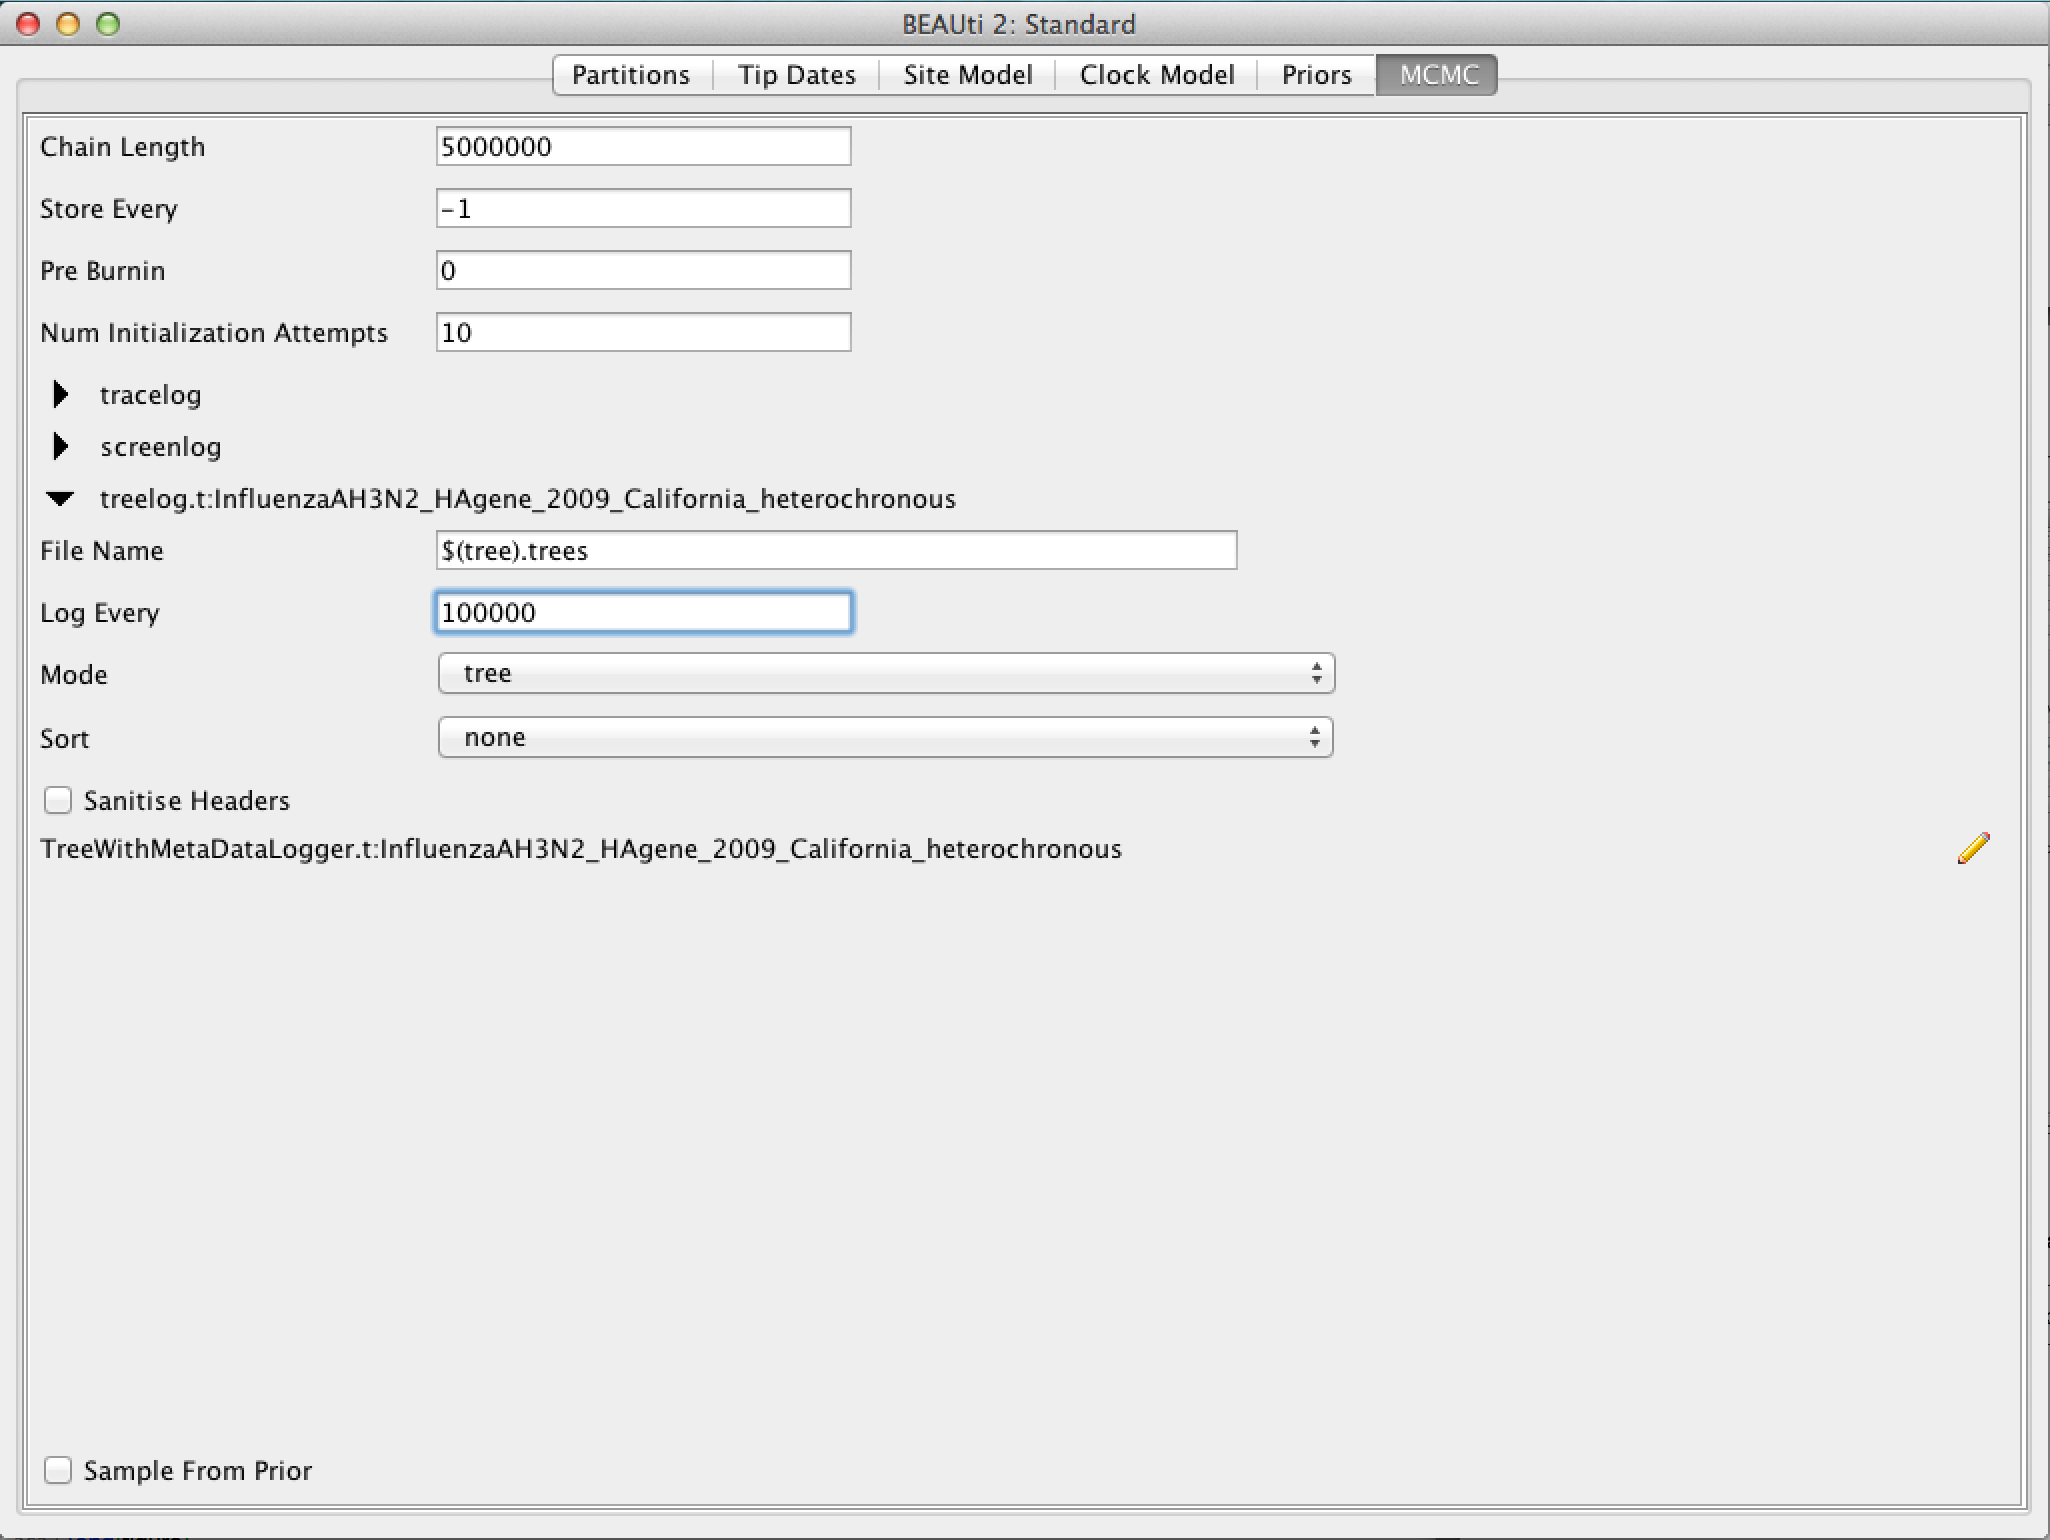
\includegraphics[width=0.75\textwidth]{figures/beast2_mcmc.png}}
\caption{\small Specifying the MCMC properties.}
\label{mcmc}
\end{figure}

Now, all the specifications are done. We want to save and run the XML.

\begin{framed}
Save the XML file as \textbf{Heterochronous.xml}
\end{framed}


\newpage
\subsubsection{Setting up the Markov Chain properties}

\begin{framed}
Within BEAST, specify the file Heterochronous.xml. %and set the random seed to 1 so that you can compare your results to the example solution.

Hit \textbf{Run} to start the analysis.
\end{framed}

The run should take about 15-20 minutes. While waiting for your results, you can start preparing the XML file for the homochronous data as specified in section \ref{homochronous}.



\bigskip
\subsubsection{Analyzing the results}

\begin{framed}
Load the file into \textbf{Tracer} to check mixing and the parameter estimates. 
\end{framed}

First thing you may notice is that most of the parameters do have low ESS (effective sample size below 200, marked in red). This is because our chain did not run long enough. However, the estimates we obtained with a chain of length 5'000'000 are very similar to those obtained with a chain of length 30'000'000.

\begin{framed}
If you like, you can compare your results with the example results we obtained with identical settings. %You can get the example result files from 
%\begin{center}
%{\textcolor{red}{\underline{\bf 
%%\url{
%the link to solution should come here
%%} 
%}}}
%\end{center}
\end{framed}

Browse the parameter estimates and reflect on them with respect to the priors we set. 



\newpage
\section{Practical: H3N2 flu dynamics - homochronous data}\label{homochronous}

We could also use the homochronous data to investigate the dynamics of the H3N2 spread in California in 2009. We use the 29 sequences from April 28, 2009 to investigate whether this is possible. 

Follow the same procedure as for the heterochronous sampling starting at section \ref{Importing alignment}. Now, however, use the alignment file called \texttt{InfluenzaAH3N2\_HAgene\_2009\_California\_homochronous.nexus} and use the \textbf{Birth Death Skyline Contemporary} model.



\bigskip
\subsection{Estimating the substitution rate from homochronous data}
After the run is finished, load the log file into Tracer. Most of the parameters have again ESS below 200. Running the analysis for longer corrects for this; however, the parameter estimates remain very similar. Now, check the clock rate and the tree height parameters. 

\begin{framed}
{\bf QUESTION: Do you think that homochronous samples allow for good substitution rate estimation? 

If yes, how would you know? 

If not, how can you see that and where do you think might the problem be? Can we address this problem in our analysis?} 
\end{framed}

Notice the values of the substitution rate estimates. From literature, one can read that influenza's HA gene has a substitution rate of about $10^{-3}$ substitutions per site per year \citep{jenkins2002}. Our estimate of the clock rate is around this value, but has a very large confidence interval. Notice also, that the confidence interval of the tree height is very large [0.1347,5.0445].

Another way to see that the homochronous sampling does not allow for the estimation of the clock rate is to observe a very strong negative correlation of the clock rate with the tree height.

\begin{framed}
In \textbf{Tracer} click on the \textbf{Joint Marginal} panel, select the \textbf{TreeHeight} and the \textbf{clockRate} simultaneously, and uncheck the \textbf{Sample only} box below the graphics [Figure \ref{clockRatetreeHeightCorrelation}].
\end{framed}

\begin{figure}[h!]
\centering
\fbox{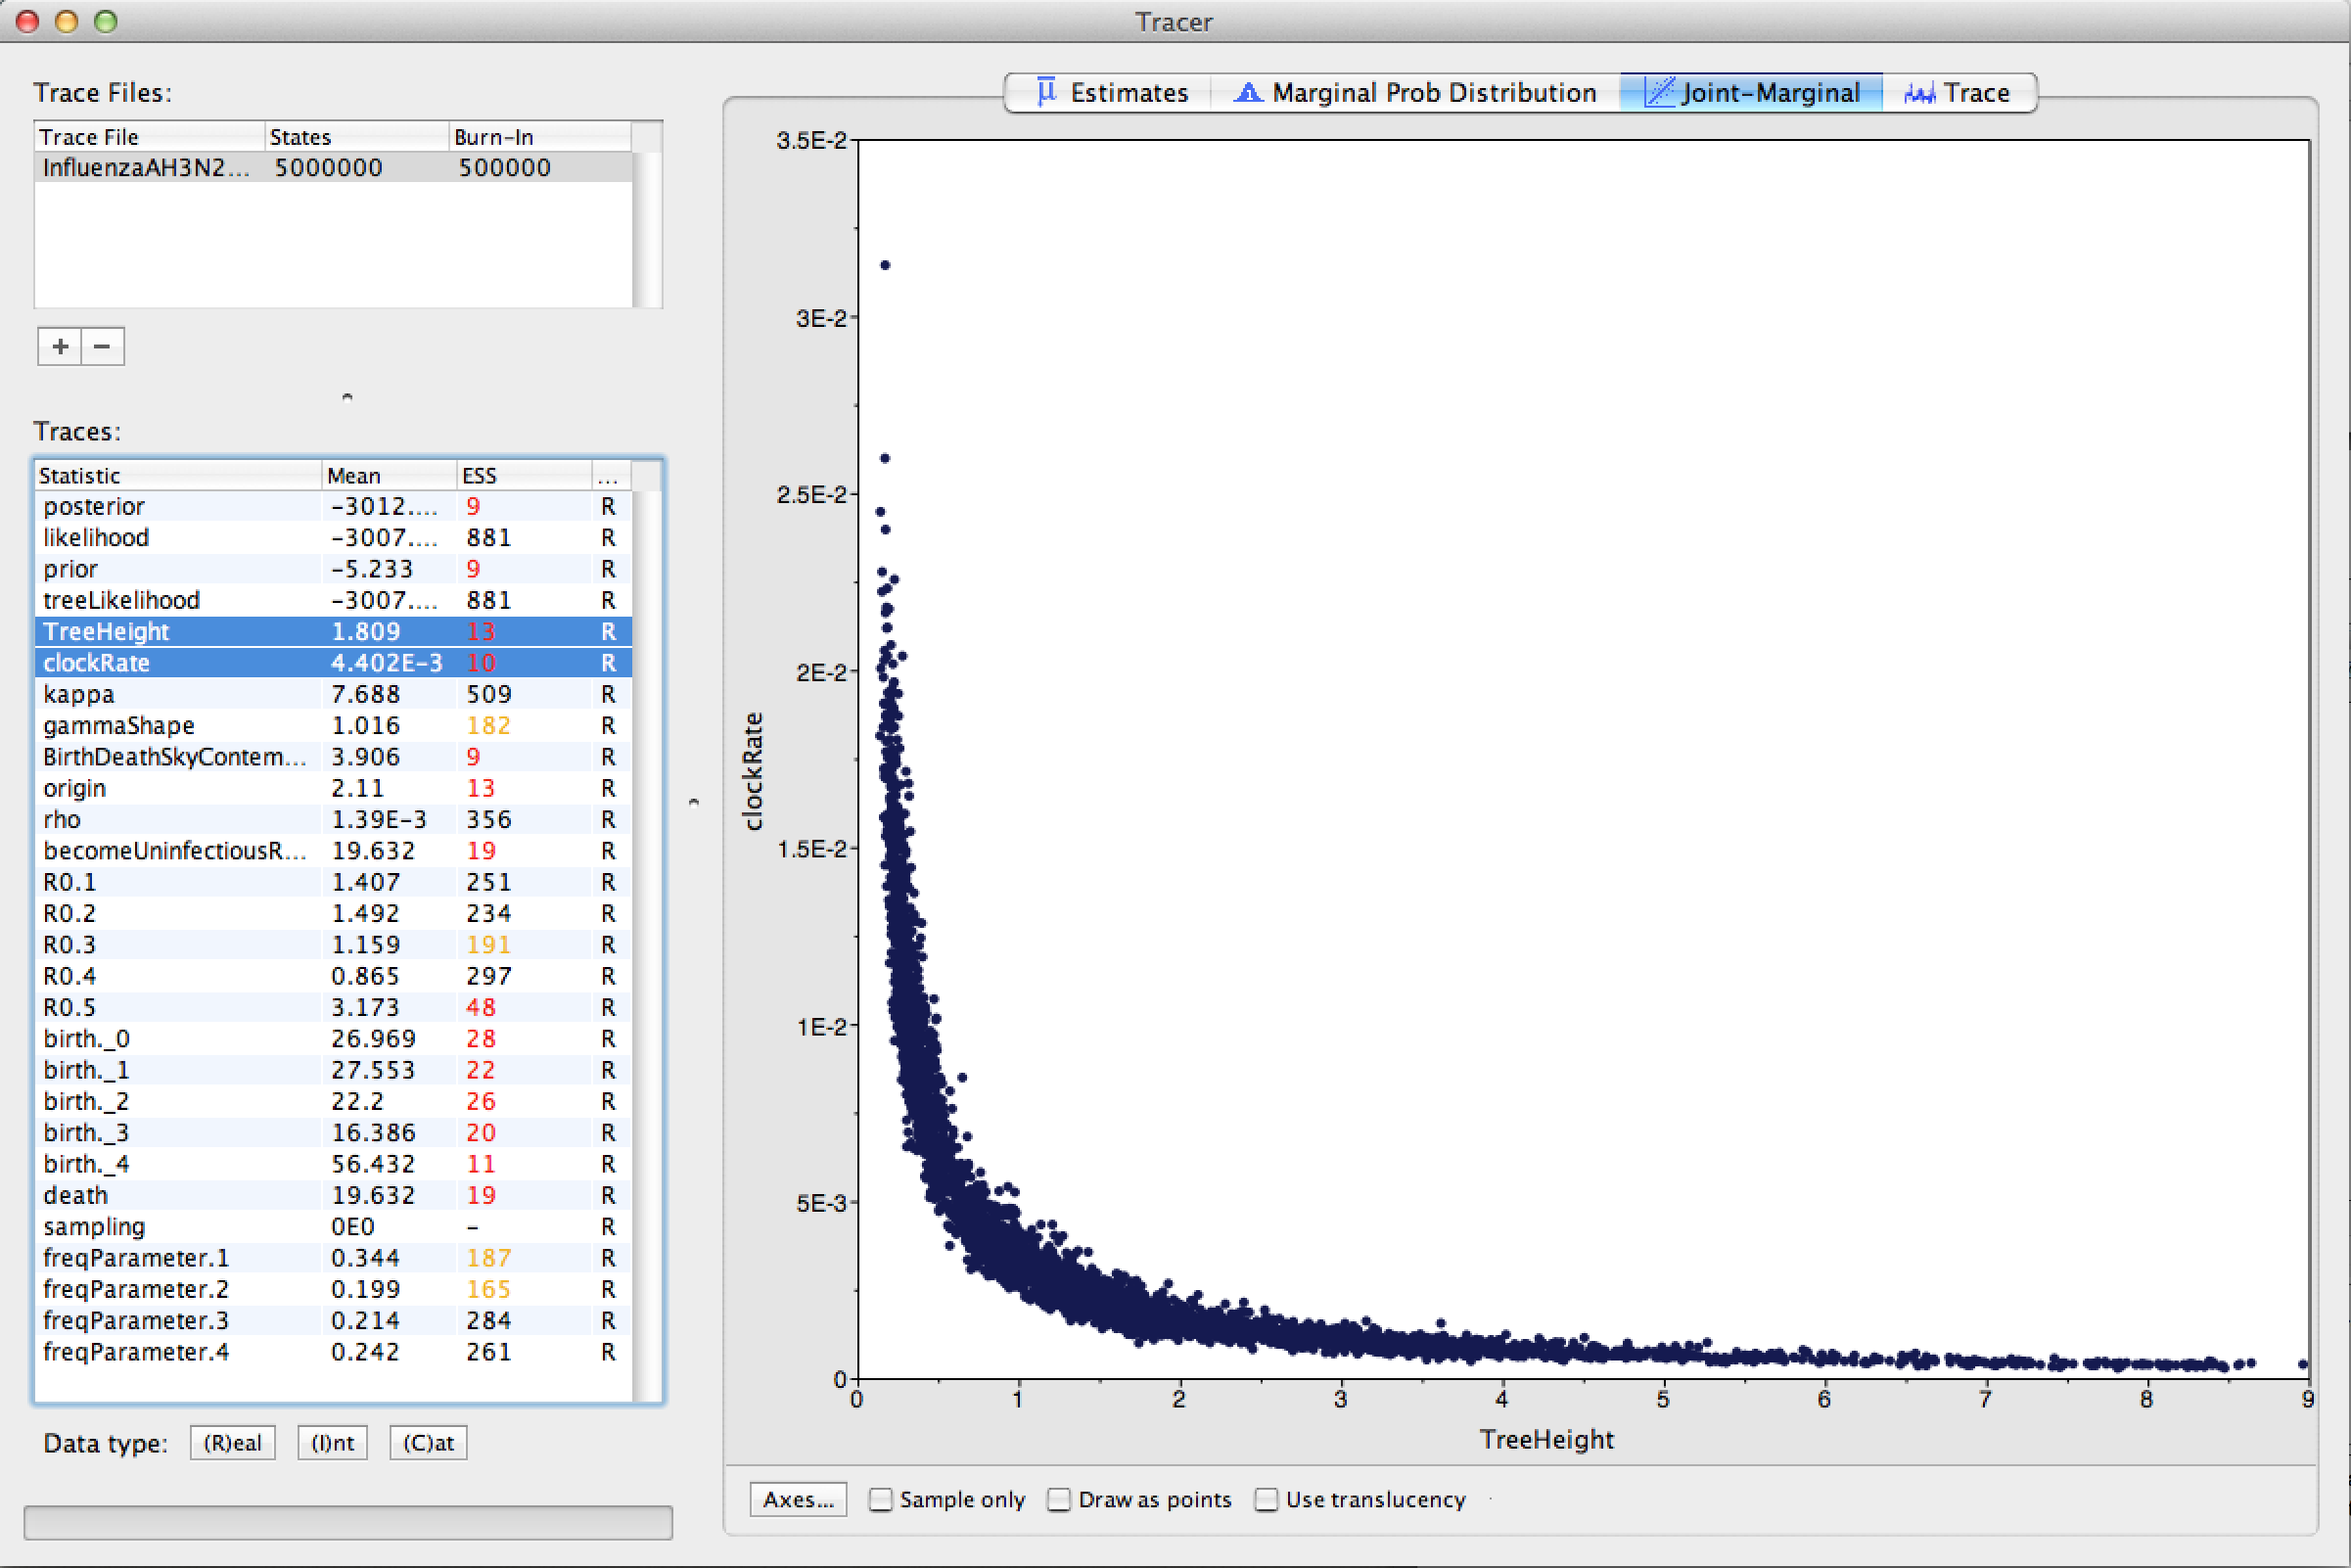
\includegraphics[width=0.75\textwidth]{figures/tracer_homochronous_treeHeightclockRatecorrelation.png}}
\caption{\small Clock rate and tree height correlation in homochronous data.}
\label{clockRatetreeHeightCorrelation}
\end{figure}

The correlation between the tree height and the clock rate is obvious: the taller the tree, the slower the clock. One way to solve this problem is to break this correlation by setting a strong prior on one of the two parameters. We describe how to set a prior on the tree height in the section below. 



\newpage
\subsubsection{Creating Taxon Sets}

We will use the results from the heterochronous data, to find out what a good estimate for the tree height of these homochronous samples is. For this aim, we first create an MCC (maximum clade credibility) tree in the \textbf{TreeAnnotator} and then check with \textbf{FigTree} what the estimate of the tMRCA (time to the most recent common ancestor) of the samples from April 28, 2009 is.

Note, however, that we do this for illustration purposes only. In a good practice, one should avoid re-using the data or using the results of an analyses to inform any further analyses containing the same data. Let's pretend therefore that the heterochronous dataset is an independent dataset from the homochronous one. 

\begin{framed}
Open the \textbf{TreeAnnotator} and set \textbf{Burnin percentage} to 10, \textbf{Posterior probability limit} to 0.5. Leave the other options unchanged.

Set the \textbf{Input Tree File} to \texttt{InfluenzaAH3N2\_HAgene\_2009\_California\_heterochronous.trees} and the \textbf{Output File} to \texttt{InfluenzaAH3N2\_HAgene\_2009\_California\_heterochronous.tree}. [Figure \ref{treeAnnotator}]
\end{framed}

\begin{figure}[h!]
\centering
\fbox{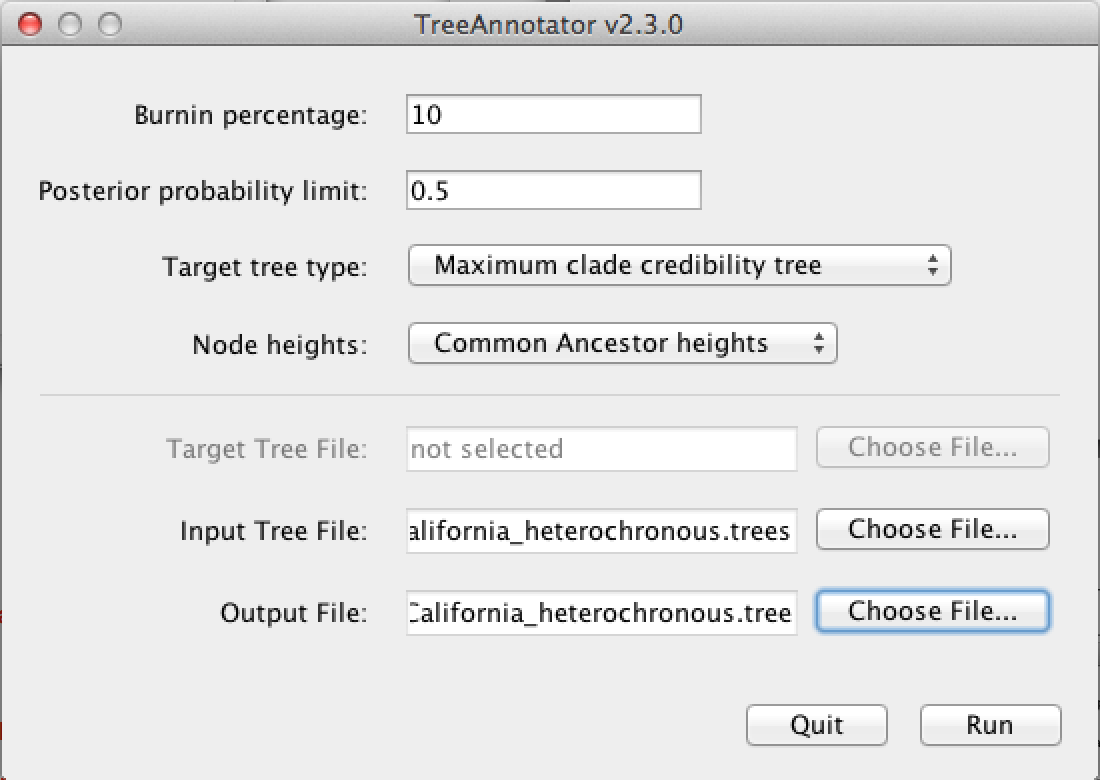
\includegraphics[width=0.5\textwidth]{figures/treeAnnotator.png}}
\caption{\small Creating the MCC tree.}
\label{treeAnnotator}
\end{figure}

\newpage
How can we find out what the tMRCA of our homochronous data may be? The best may be to have a look at the estimates of the heterochronous data in the \textbf{FigTree}.

\begin{framed}
Now open the \textbf{FigTree} and load \texttt{InfluenzaAH3N2\_HAgene\_2009\_California\_heterochronous.tree}.

In the upper right corner, next to the magnifier glass sign, type \textbf{2009/04/28} to highlight all the sequences from April 28, 2009. [Figure \ref{tMRCAmedian}]
\end{framed}

\begin{figure}[h!]
\centering
\fbox{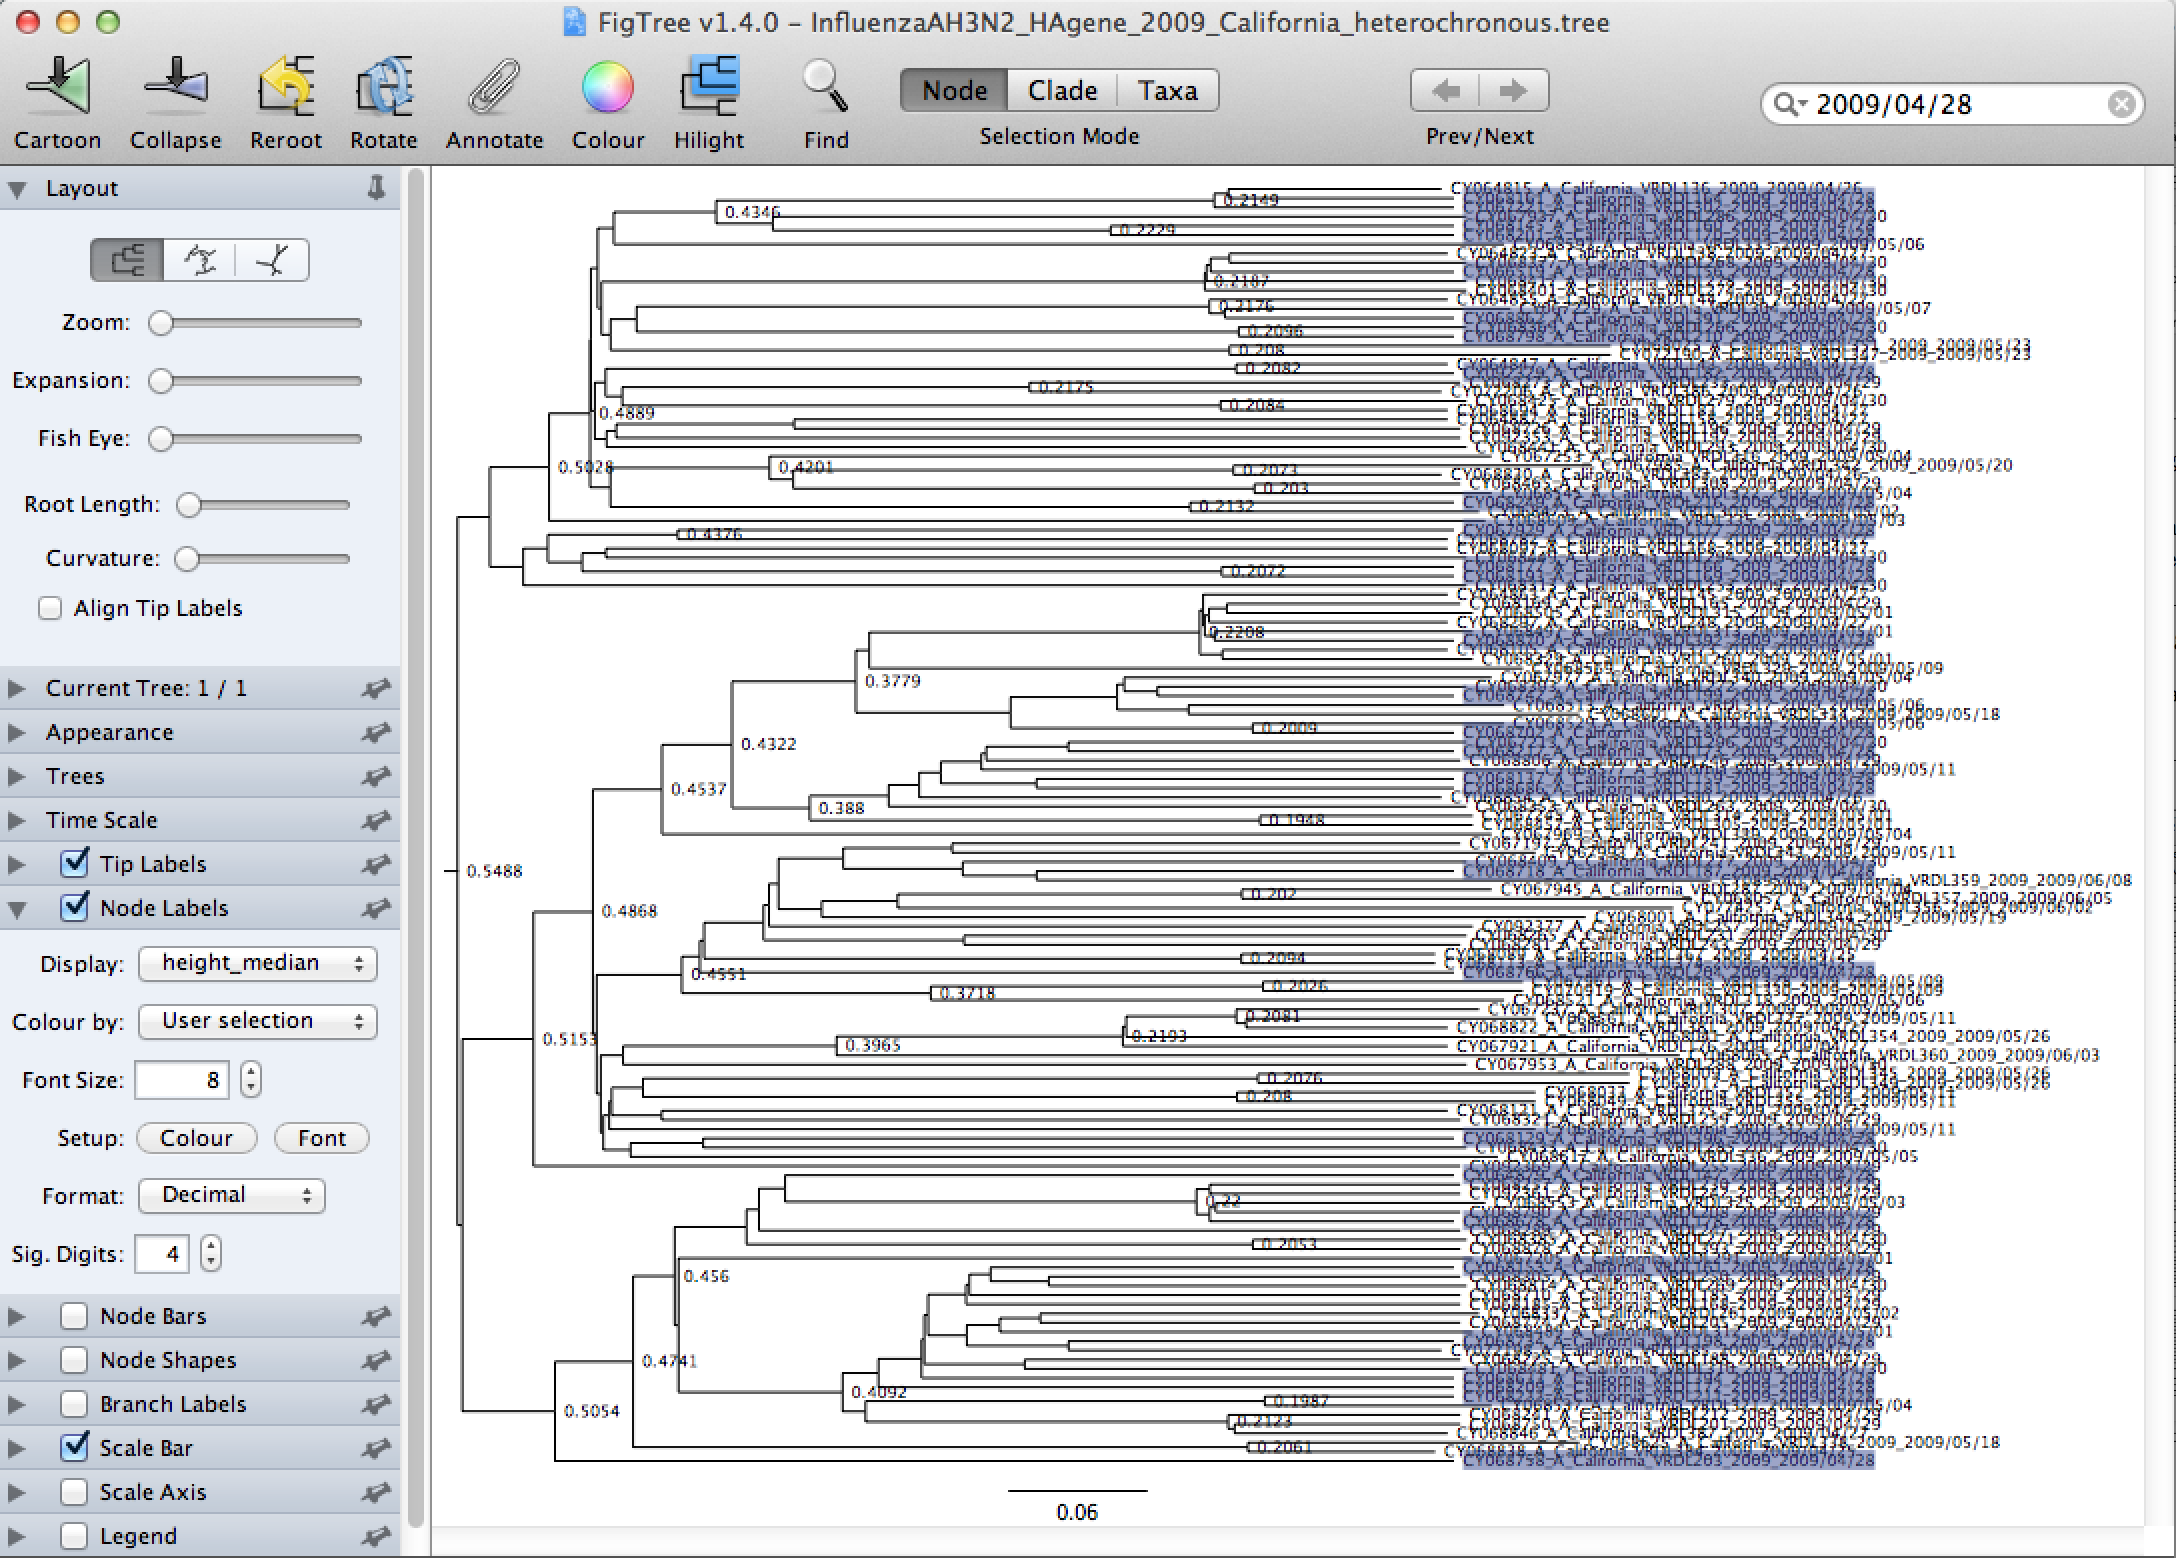
\includegraphics[width=0.75\textwidth]{figures/FigTree_tMRCA_median.png}}
\caption{\small Displaying median estimates of the node height in the MCC tree.}
\label{tMRCAmedian}
\end{figure}

\begin{framed}
Tick the \textbf{Node Labels} in the left menu, and click the arrow next to it to open the full options. Change the \textbf{Display} from \textbf{age} to \textbf{height\_median} [Figure \ref{tMRCAmedian}] and then to \textbf{height\_95\%\_HPD} [Figure \ref{tMRCA95HPD}].
\end{framed}

\begin{figure}[h!]
\centering
\fbox{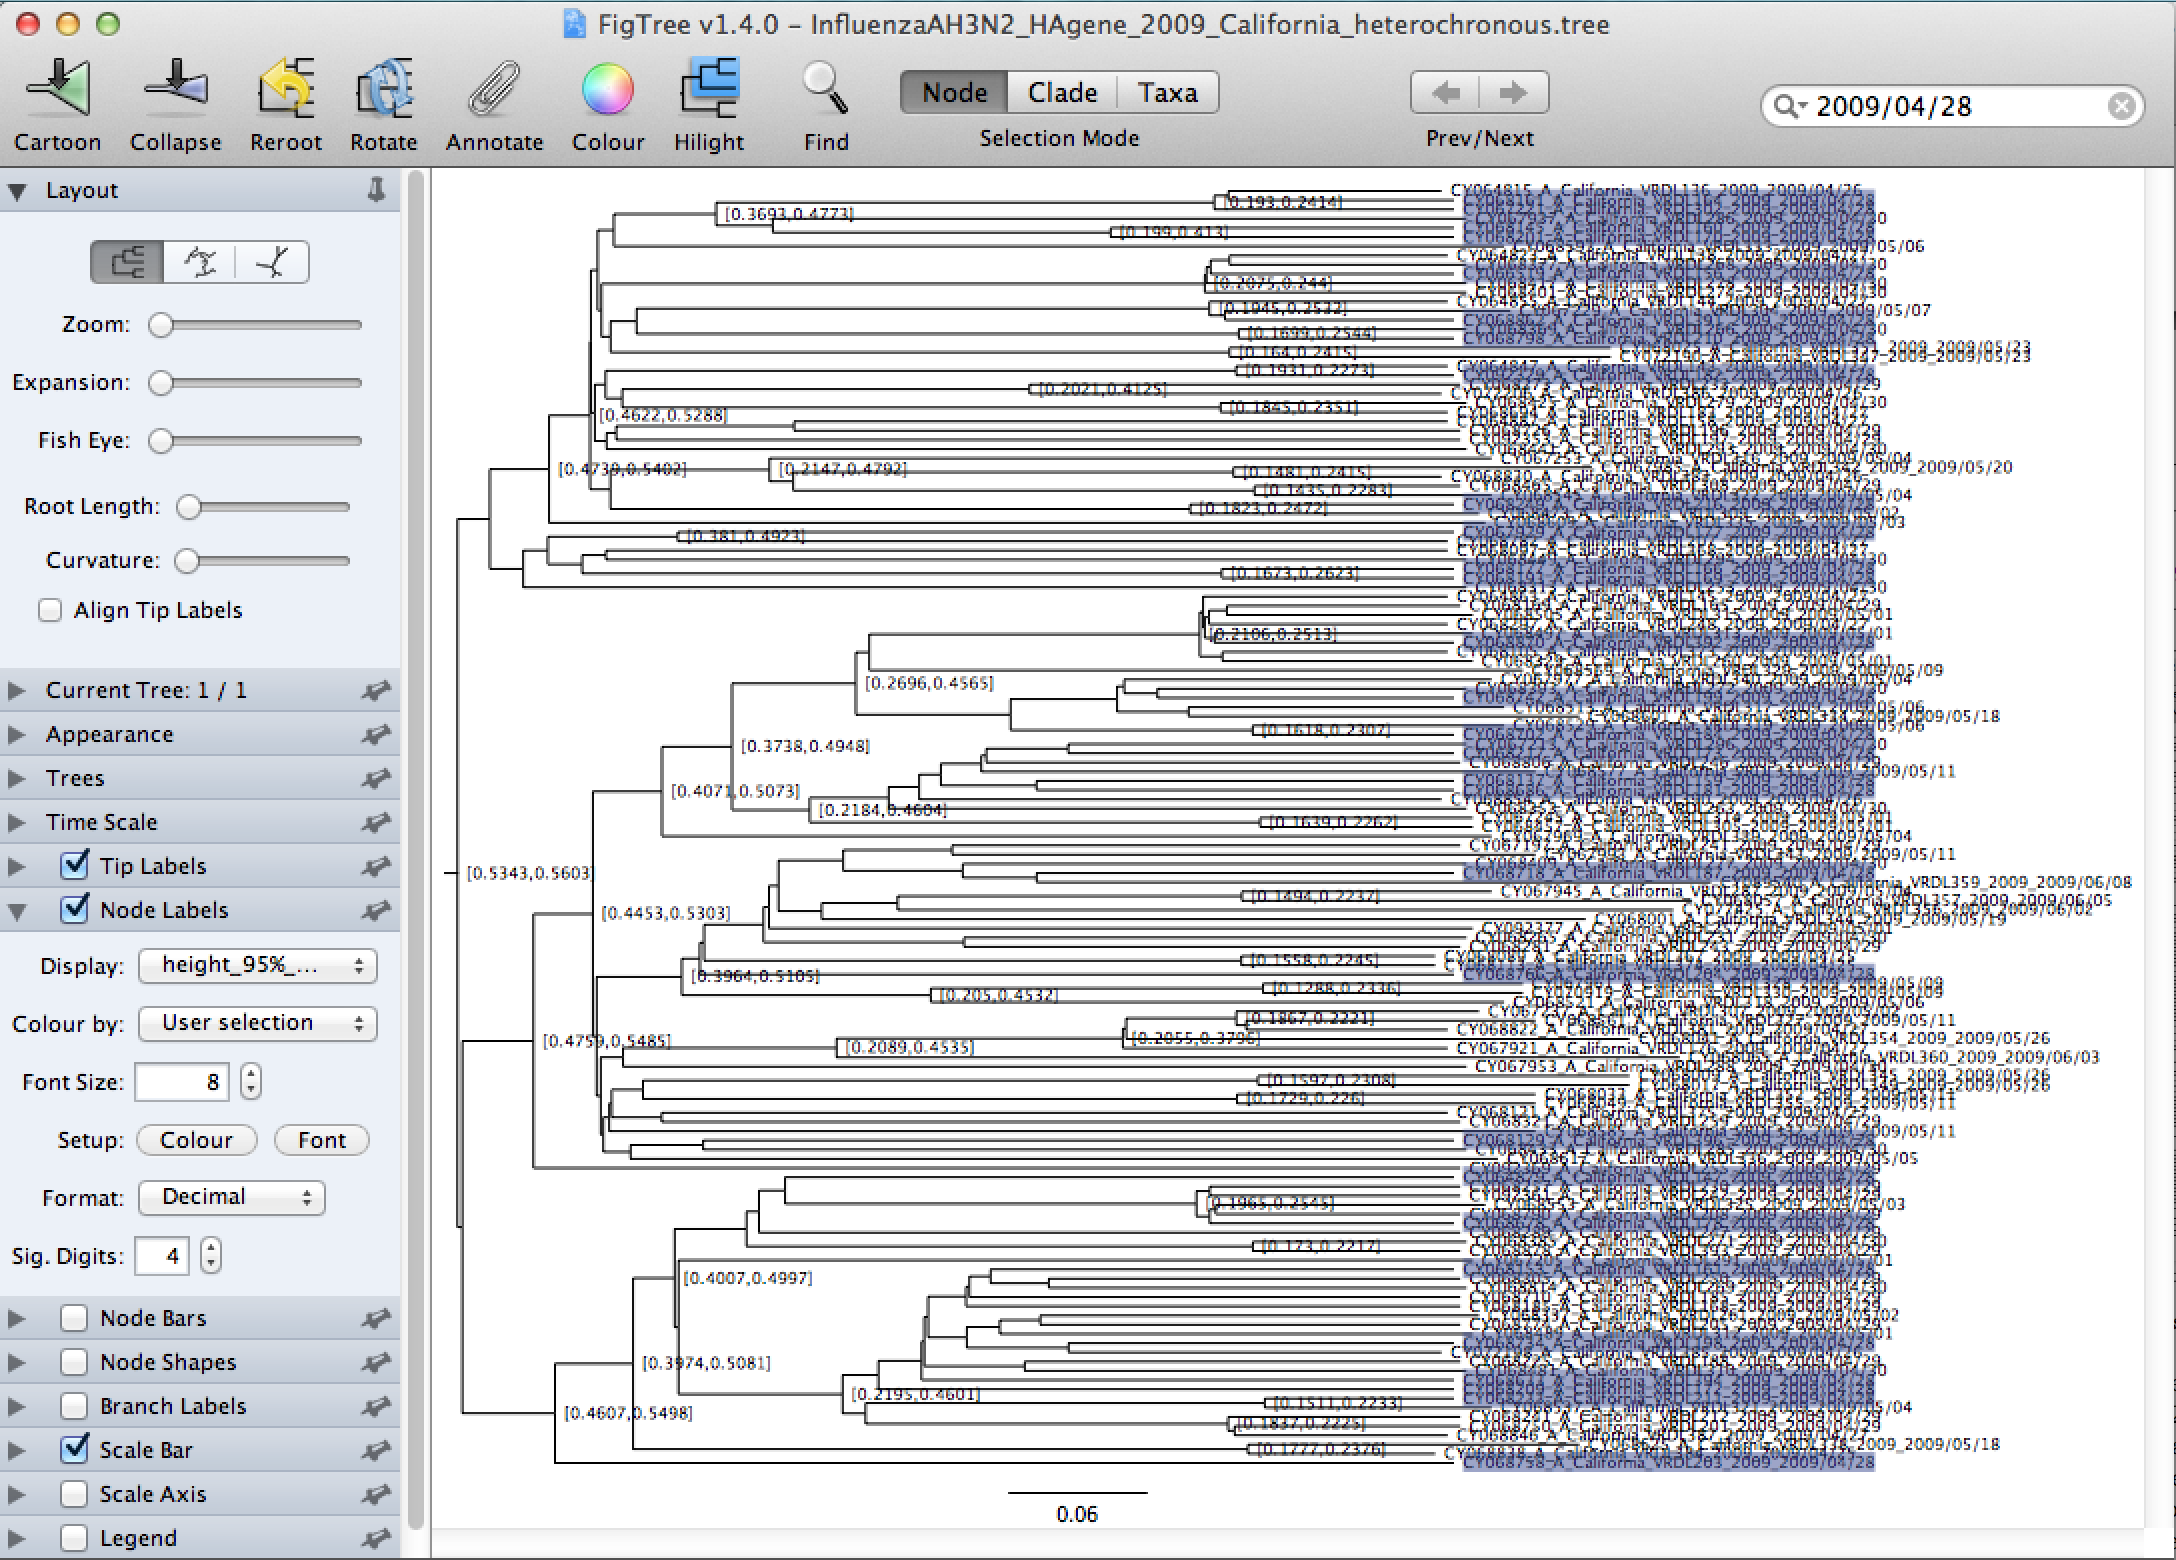
\includegraphics[width=0.75\textwidth]{figures/FigTree_tMRCA_HPD.png}}
\caption{\small Displaying 95\% HPD estimates of the node height in the MCC tree.}
\label{tMRCA95HPD}
\end{figure}

Notice, that since we are using only a subset of all the heterochronous sequences from section \ref{heterochronous}, we are interested in the tMRCA of the samples from April 28, 2009 which may not coincide with the tree height of all the heterochronous data. These samples are spread around over all the clades in the tree, and the most recent common ancestor of all of them turns out to be the root of the MCC tree of the heterochronous samples. We therefore want to set the tMRCA prior of the tree formed by the homochronous sequences to be peaked around the median value of the MCC tree height, which is 0.5488 and we want 95\% of the density of the prior distribution to be between $0.5343-0.5603$.

\begin{framed}
Open BEAUti, load the homochronous data and use the same settings as for the \texttt{Homochronous.xml} file.

Create a new taxon set for root node by clicking the \fbox{+} at the bottom of the parameter list in the \textbf{Priors} window. This will reveal the \textbf{Taxon set  editor}.

Change the \textbf{Taxon set} label to \textbf{allseq}.

Select the sequences belonging to this clade, i.e. all the tips, and move them from the left column to the right column using the \fbox{> >} button and click \textbf{OK}. [Figure \ref{tMRCAPrior}] 
\end{framed}

\begin{figure}[h!]
\centering
\fbox{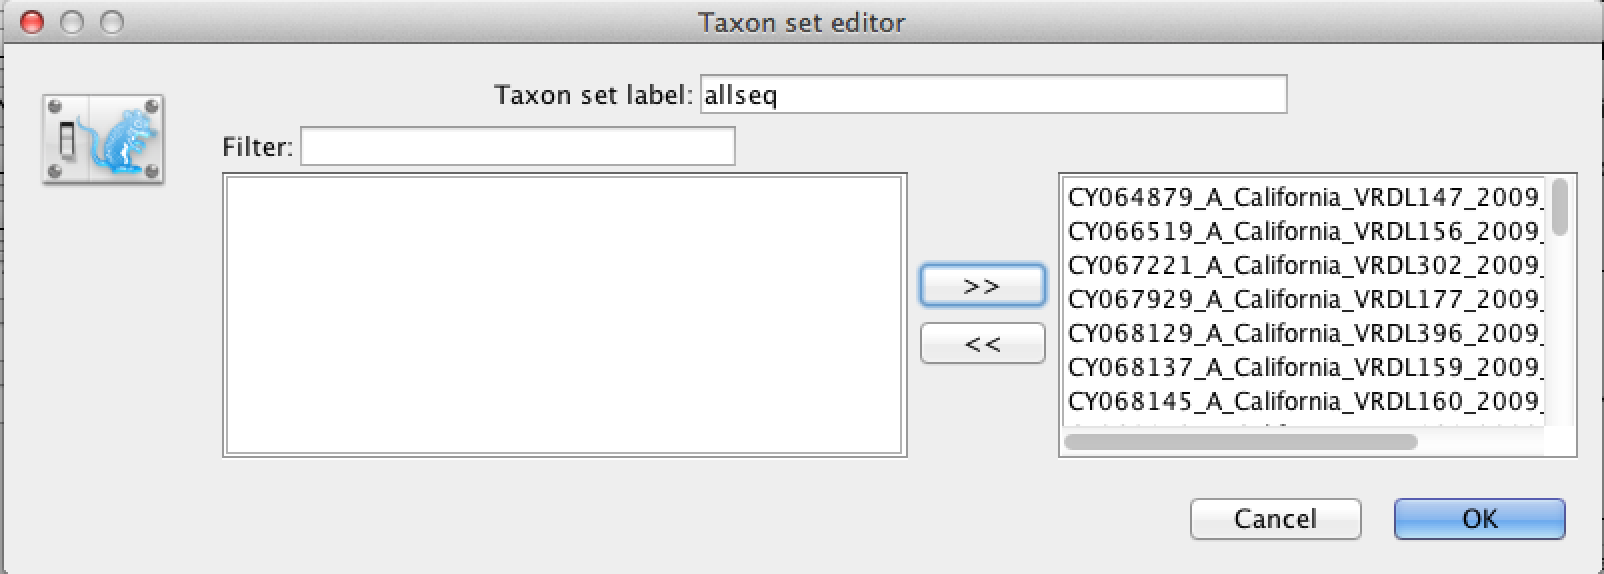
\includegraphics[width=0.75\textwidth]{figures/beast2_homochronous_tMRCA.png}}
\caption{\small Specifying the root height prior.}
\label{tMRCAPrior}
\end{figure}

The prior that we are specifying is the date (not the height) of the tMRCA of all the samples in our dataset. Thus, we need to recalculate the date from the tMRCA height estimates that we obtained above. All the tips are sampled at the date $\approx$ 2009.3233. The median date of the MRCA should therefore be calculated as follows $2009.3233-0.5488 = 2008.7745$ and the 95\% HPD should be $[2009.3233-0.5603,2009.3233-0.5343]=[2008.763,2008.789]$.

\begin{framed}
Back in the \textbf{Priors} window, check the box labeled \textbf{monophyletic} for the \textbf{allseq.prior}.

Click on the arrow next to the \textbf{allseq.prior}. Change the prior distribution on the time of the MRCA of selected sequences from \textbf{[none]} to \textbf{Laplace Distribution} and set the \textbf{Mu} to 2008.7745 and the \textbf{Scale} to 0.01 [Figure \ref{tMRCAPrior2}]. 

You can check that these settings correspond to the height of tMRCA from the MCC tree by setting \textbf{Mu} to 0.5488 and observing the distribution to the right. When you are done, do not forget to set \textbf{Mu} back to 2008.7745.
\end{framed}

\begin{figure}[h!]
\centering
\fbox{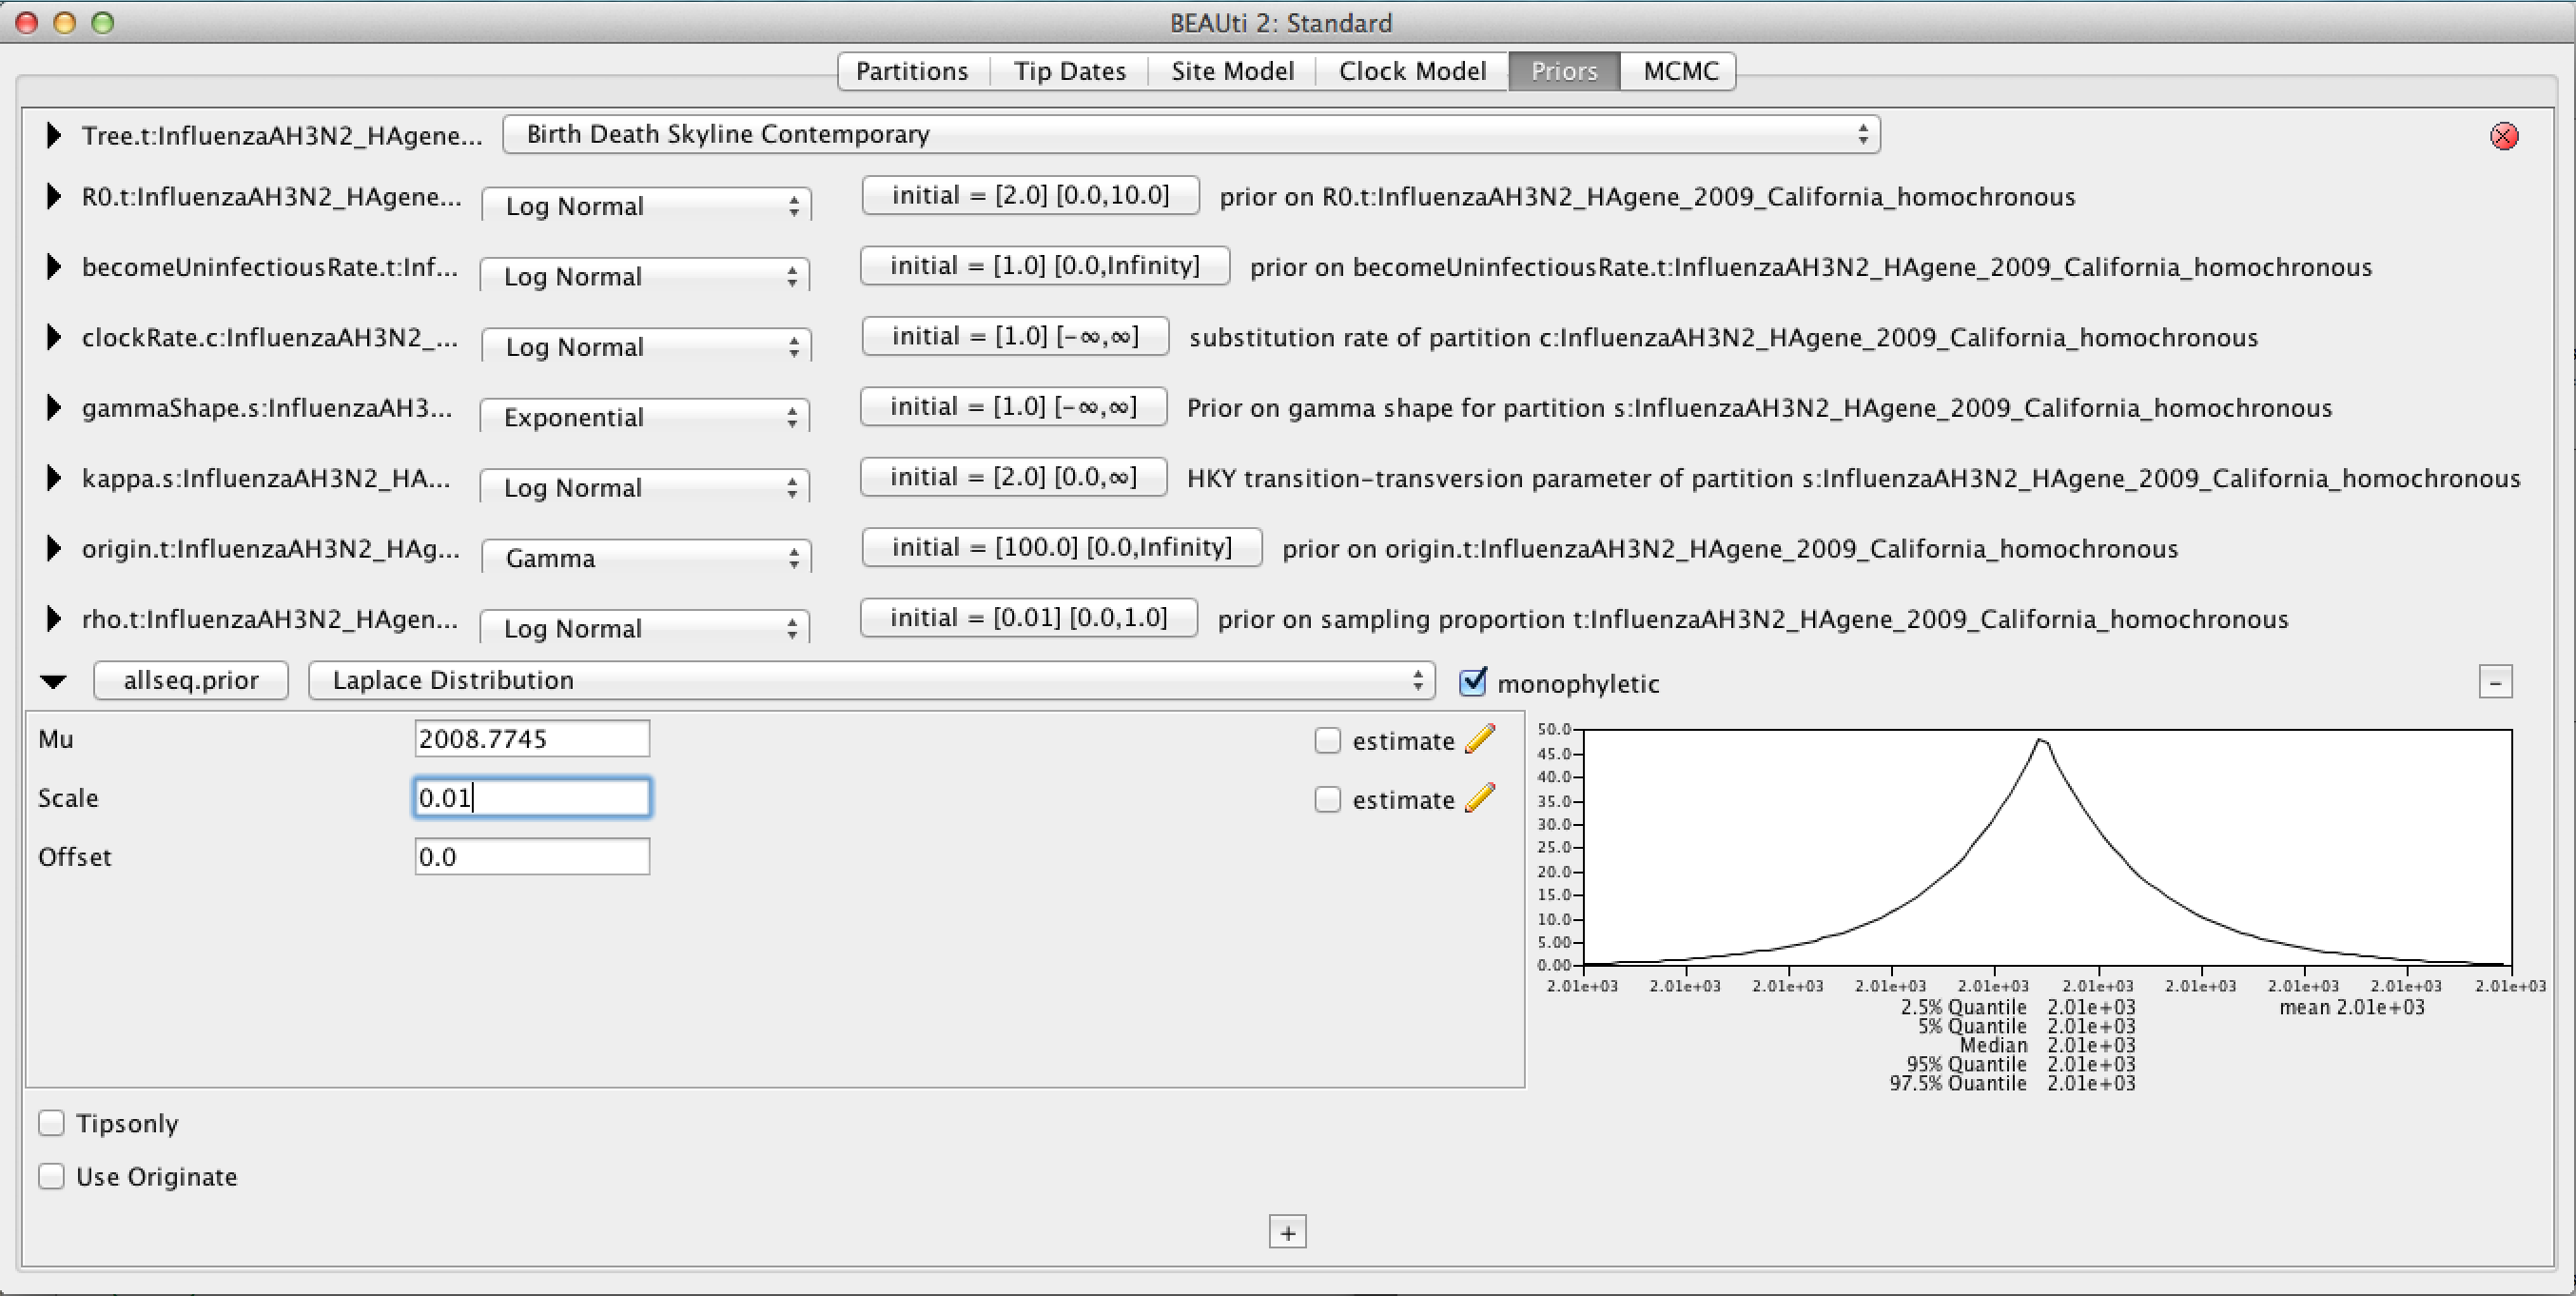
\includegraphics{figures/beast2_homochronous_tMRCA_prior.png}}
\caption{\small Specifying the root height prior.}
\label{tMRCAPrior2}
\end{figure}

We also need to change the names of the output files so that we do not overwrite the results of the previous analyses.

\begin{framed}
In the \textbf{MCMC} window, click on the arrow next to the \textbf{tracelog} and change the \textbf{File Name} to \texttt{InfluenzaAH3N2\_HAgene\_2009\_California\_homochronous\_tMRCA.log}.

Then, click on the arrow next to the \textbf{treelog} and add \texttt{\_tMRCA} between \texttt{\$(tree)} and \texttt{.trees} in the \textbf{File Name} field. [Figure \ref{tMRCAPrior3}]
\end{framed}

\begin{figure}[h!]
\centering
\fbox{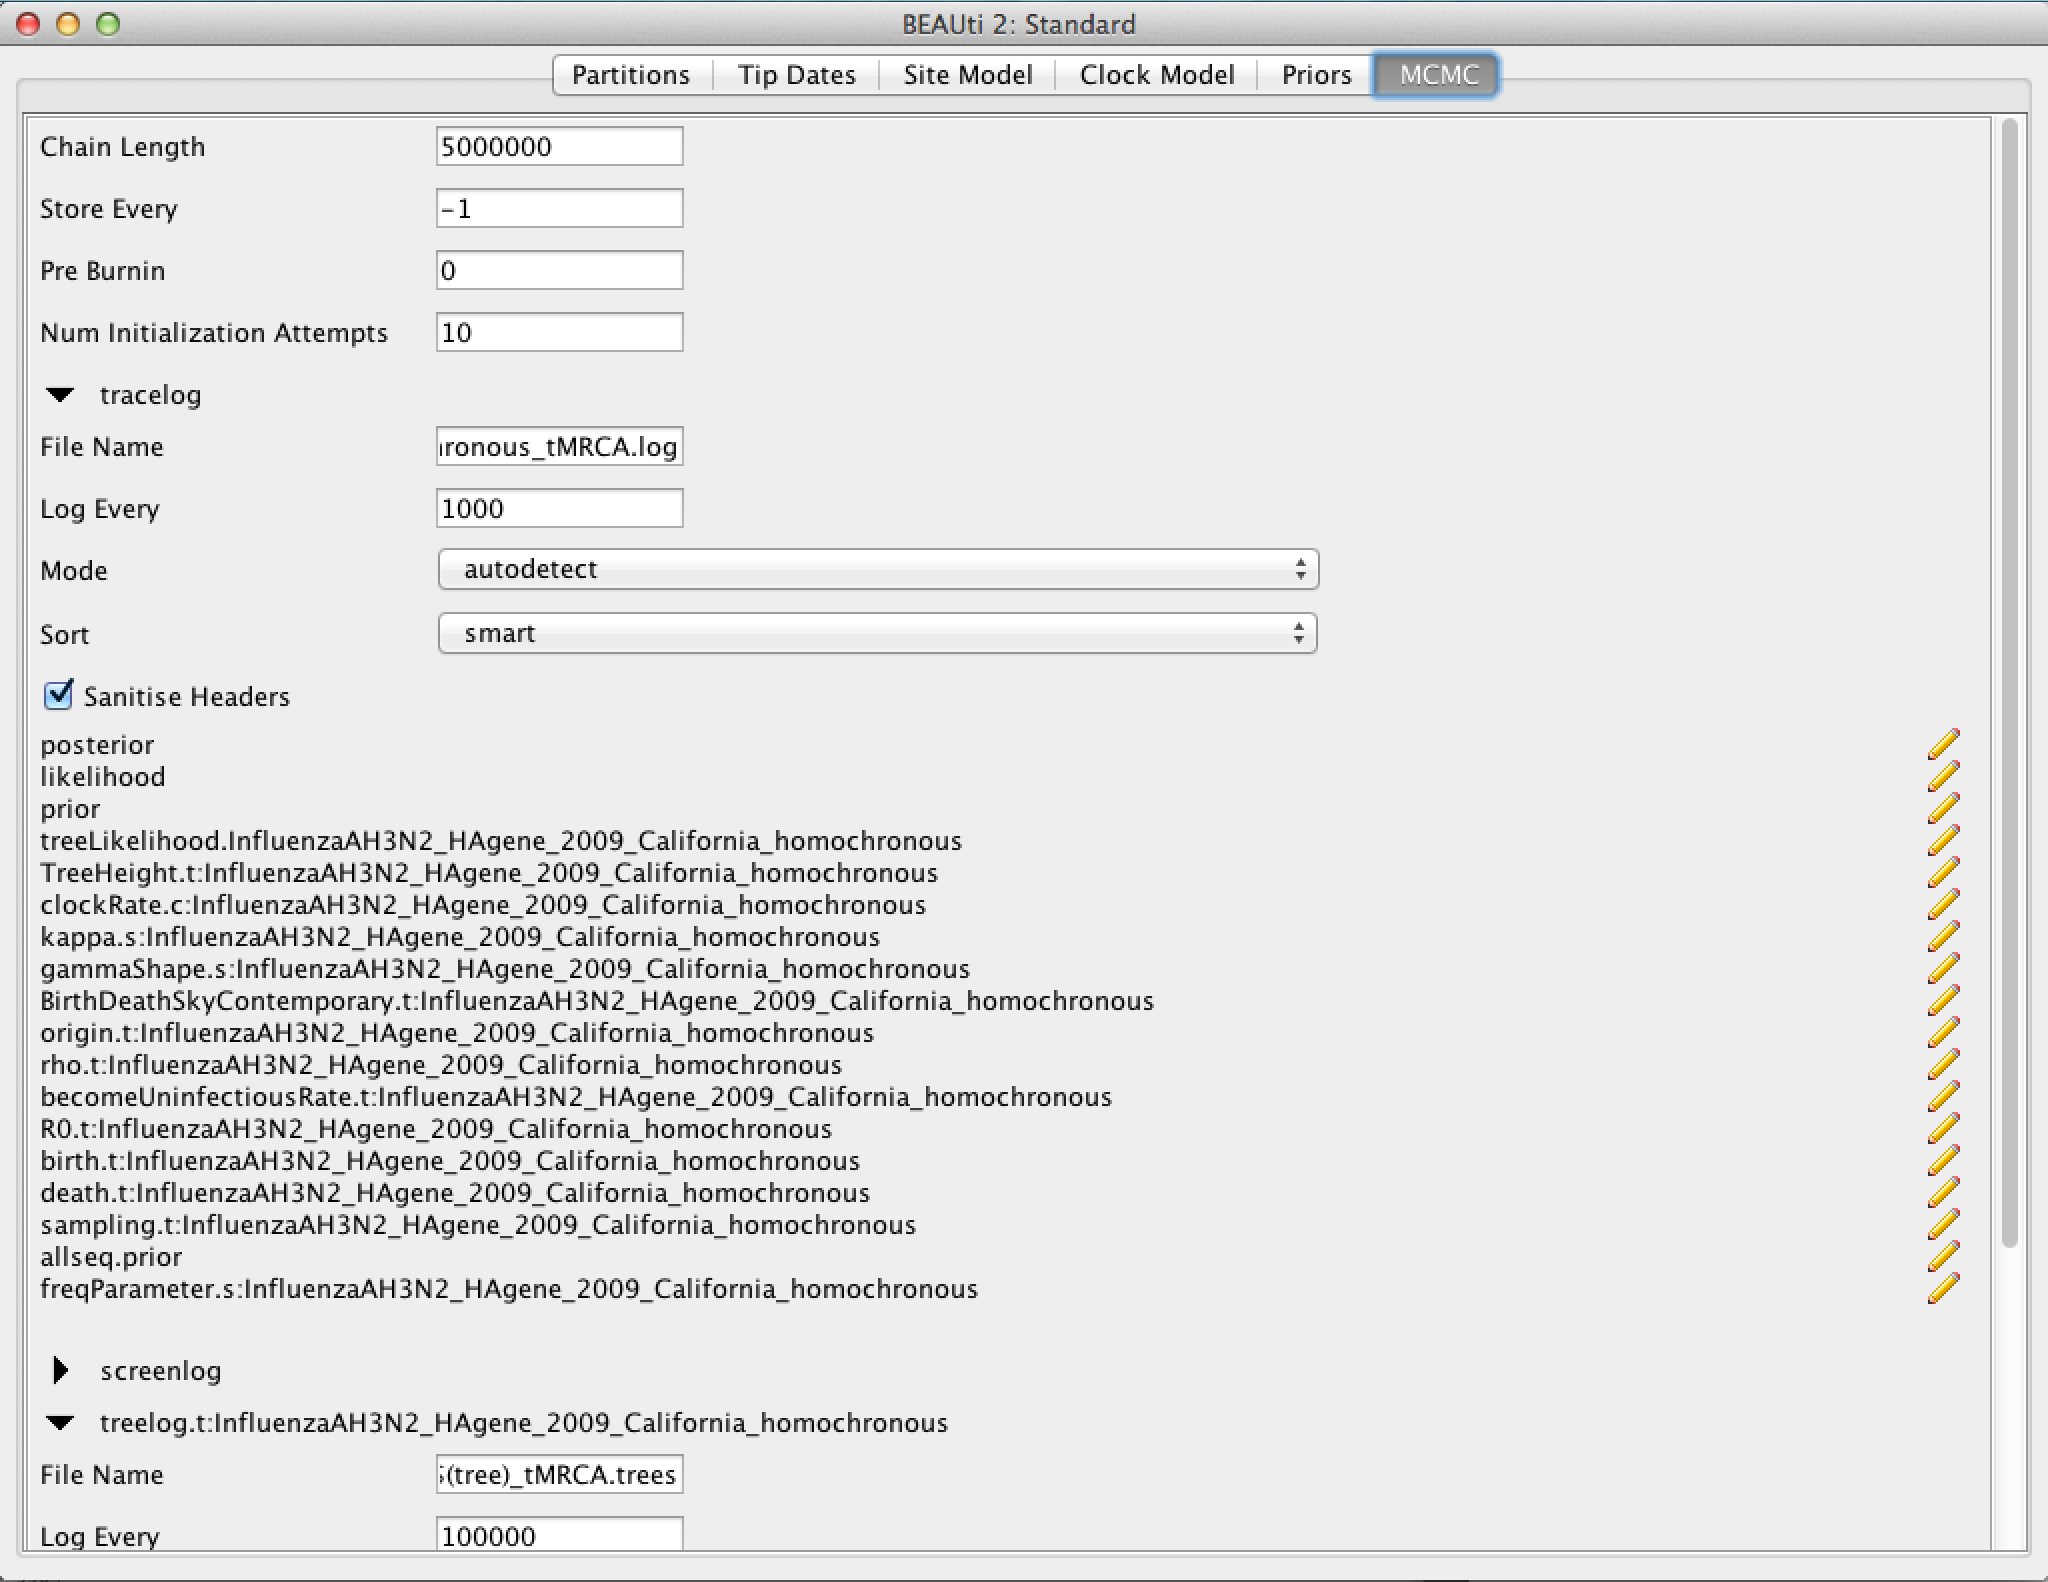
\includegraphics[width=0.75\textwidth]{figures/beast2_homochronous_tMRCA_files.png}}
\caption{\small Specifying the output file names.}
\label{tMRCAPrior3}
\end{figure}

\newpage
Run the analysis and compare to the original analysis of the homochronous data. Are the substitution rate estimates more precise now?

%%%%%
\newpage
\bigskip
\section{Useful Links}

\begin{itemize}
\item \href{http://www.beast2.org/book.html}{\textit{Bayesian Evolutionary Analysis with BEAST 2}}  \citep{BEAST2book2014}\\ \vspace{-7mm}
\item BEAST 2 website and documentation: \href{http://www.beast2.org/}{http://www.beast2.org/} \\ \vspace{-7mm}
\item BEAST 1 website and documentation: \href{http://beast.bio.ed.ac.uk}{http://beast.bio.ed.ac.uk} \\ \vspace{-7mm}
\item Join the BEAST user discussion: \href{http://groups.google.com/group/beast-users}{http://groups.google.com/group/beast-users} \\ \vspace{-7mm}
\end{itemize}

%Questions about this tutorial can be directed to Tracy Heath (email: \href{mailto:tracyh@berkeley.edu}{tracyh@berkeley.edu}).

\href{http://creativecommons.org/licenses/by/4.0/}{
\includegraphics[scale=0.8]{figures/ccby.pdf}} This tutorial was written by %\href{google.com}
{Veronika Bo\v{s}kov\'a and Venelin Mitov} for the \href{https://www.bsse.ethz.ch/cevo/taming-the-beast.html}{Taming the BEAST Workshop} on applied phylogenetics and molecular evolution and is licensed under a \href{http://creativecommons.org/licenses/by/4.0/}{Creative Commons Attribution 4.0 International License}. 



Version dated: \today



%\nocite{hug07,inoue10,magallon09,marshall08,ronquist11,rutschmann07,lee09,li12,drummond07,gaut94,hasegawa89,muse92,rannala96,rannala07,sanderson97,sanderson02,sukumaran10,thorne05,yang97b,yang06,yoder00,benton03,graur04,ho07,hugall07,kishino90b,marshall90,stadler09,stadler10,stadler11,warnock12,pyron11,dosReis2012,dosReis2013,dosReis2011,arisbrosou03,arisbrosou02,baele12,baele13,benton00,brown11,Cutler2000a,Cutler2000,Darriba2013,doyle93,drummond2003,fan11,gandolfo08,Guindon2010,Hohna2012,hohna11,hasegawa85,hastings70,heath08b,heath08,Himmelmann2009,ho11,hull88,lartillot2013,lartillot2011,lartillot2012,lloyd12,lukoschek12,Morlon2011,Nylander2008,Parham2012,robinson98,rodrigo2003,shapiro11,Stadler2011,Stadler2013,Suchard2003,tajima93,Thorpe1982,weir2008,welch05,wilkinson11,xie11,Zuckerkandl1965,HeathMoore2013}


\newpage

%%%%%%%%%%%%%%%%%%%%%%%%%%%%%%%%%%%%
%  REFERENCES  
%%%%%%%%%%%%%%%%%%%%%%%%%%%%%%%%%%%%

\printbibliography[heading=relevref]




\end{document}
